\documentclass[10pt]{report}
\usepackage[utf8]{inputenc}
\usepackage{amsmath,mathtools}
\usepackage{tcolorbox}
\newcommand{\mbf}[1]{\mathbf{#1}}
\newcommand{\tbf}[1]{\textbf{#1}}
\newcommand{\dsum}[3]{$\sum^{#1}_{#2}{#3}$}
\newcommand{\dint}[3]{\int^{#1}_{#2}{#3}}
\newcommand{\tit}[1]{\textit{#1}}
\newcommand{\fn}[1]{\footnote{#1}}
\newcommand{\de}[2]{\frac{d{#1}}{d{#2}}}
\newcommand{\ch}[2]{\Gamma^{#1}_{#2}}
\newcommand{\chris}{\ch{\mu}{\alpha \beta}=\frac{1}{2}g^{\mu \lambda}(\p_{\alpha} g_{\beta \lambda}+\p_\beta g_{\alpha \lambda} - \p_\lambda g_{\alpha \beta})}
\newcommand{\p}{\partial}
\newcommand{\pe}[2]{\frac{\partial{#1}}{\partial{#2}}}
\newcommand{\n}{\nonumber}
\newcommand{\cbox}{tcolorbox}
\newcommand{\cc}[1]{\left({#1}\right)}
\newcommand{\rr}[1]{\left[{#1}\right]}
\newcommand{\aab}[1]{\left\langle{#1}\right\rangle}
\begin{document}
\title{Radio Astronomy Techniques}
\author{Divesh Jain}
\maketitle
\tableofcontents
\chapter{Brief Introduction to everything in this notes}
\section{Why Interferometry?}
\subsection{The field of Observational science and requirements}
To answer this, it is helpful to return to the basic requirements for any instrument used to observe astronomical sources at any wavelength. Good resolution and accurate intensity values, in other words, good signal to noise measures are essential for any science. \\

\tbf{What does an optical telescope do?}\\
An optical telescope measures the number of photons collected, and hence the signal to noise achievable depends on the diameter of the dish. 

\tbf{How does a radio telescope work?}\\
A radio receiver measures the voltage induced by the radio signal received, and again, the wider the collecting area, the stronger the signal. Looking at the resolution however, classical optical diffraction theory limits the angular resolution achievable by a single dish telescope to
\begin{equation}
\theta\sim \frac{\lambda}{D}
\end{equation}
where $\lambda$ is the wavelength of the radiation received , and D is the diameter of the telescope. 

\tbf{Q. what is interferometry in a lay man's language?}\\

The very basic key concept behind an interferometer is that one can link many single radio dishes together, combining the signal received at each, and effectively simulating a large single radio telescope dish, with a diameter equivalent to the largest distance (baseline) between the smaller dishes.
\section{Some Basic Physics and a picture based Introduction}
\tbf{First we attempt with understanding Young's Double split before getting into Radio fringes}\\

A monochromatic source of light passing through two slits will diffract, and produce a fringe pattern of maxima and minima, an angular distance $\lambda$/d apart. The phase difference between waves will change as the path lengths taken vary, giving rise to the constructive $\&$ destructive interference seen on the viewing screen. Check the figure on YDS Figure \ref{yds}
\begin{figure}\label{yds}
\includegraphics[scale=1]{yds.png}
\end{figure}

\tbf{Interferometers and fringe pattern}\\

Now, Interferometers use exactly the same concept. First consider the simplest interferometer, composed of two antennas, as illustrated in Figure \ref{ap}. Everything we can learn about a source in the sky comes from the distribution of it;s electric field. Each antenna measures a different part of the wavefront arriving from the source. The signals from each antenna are cross-correlated, and analogous to the Young's slits experiments above, depending on the path taken and the distance between the antennas, the interferometer output will either be constructive or destructive. If we add in the Earth's rotation to this picture, one can imagine a source moving through the interferometer beam, giving positive and negative output, and producing a fringe pattern as in Fig. \ref{ap} and Fif. \ref{baslines}.
\begin{figure}\label{ap}
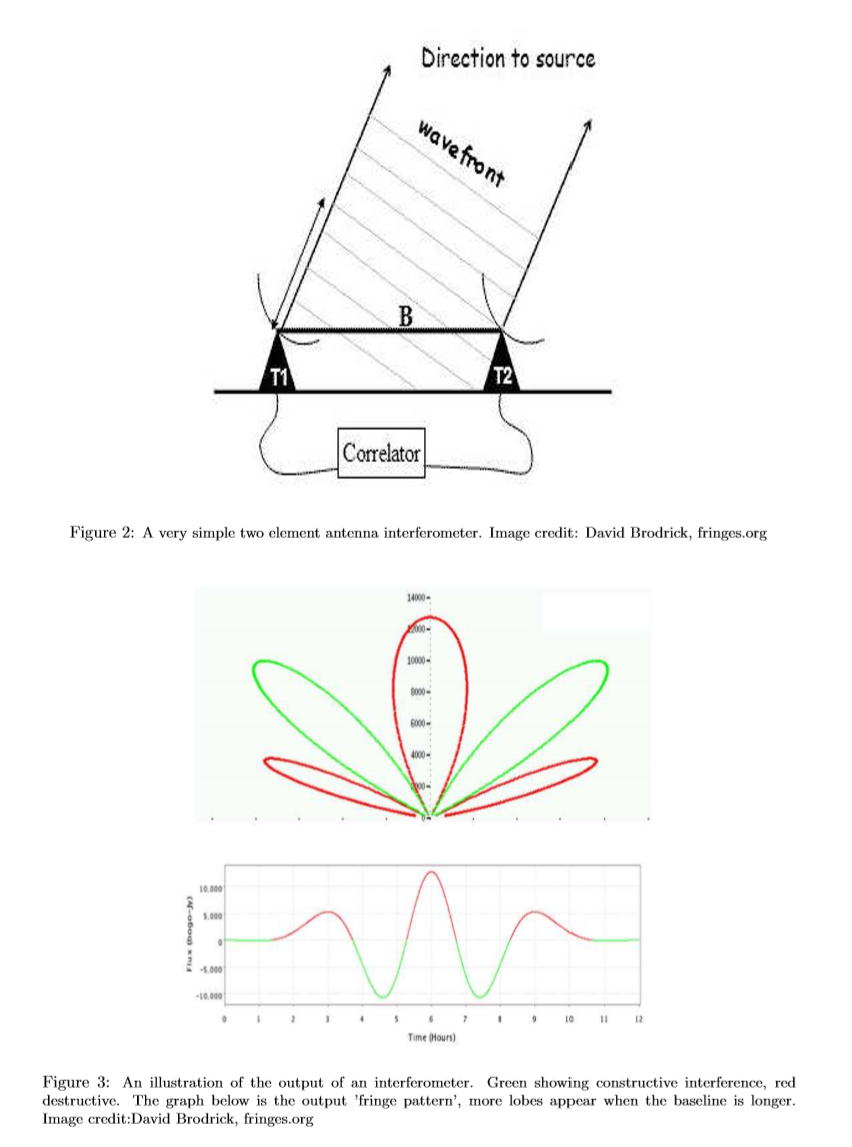
\includegraphics[scale=1]{antennapattern.png}
\end{figure}

\begin{figure}\label{baslines}
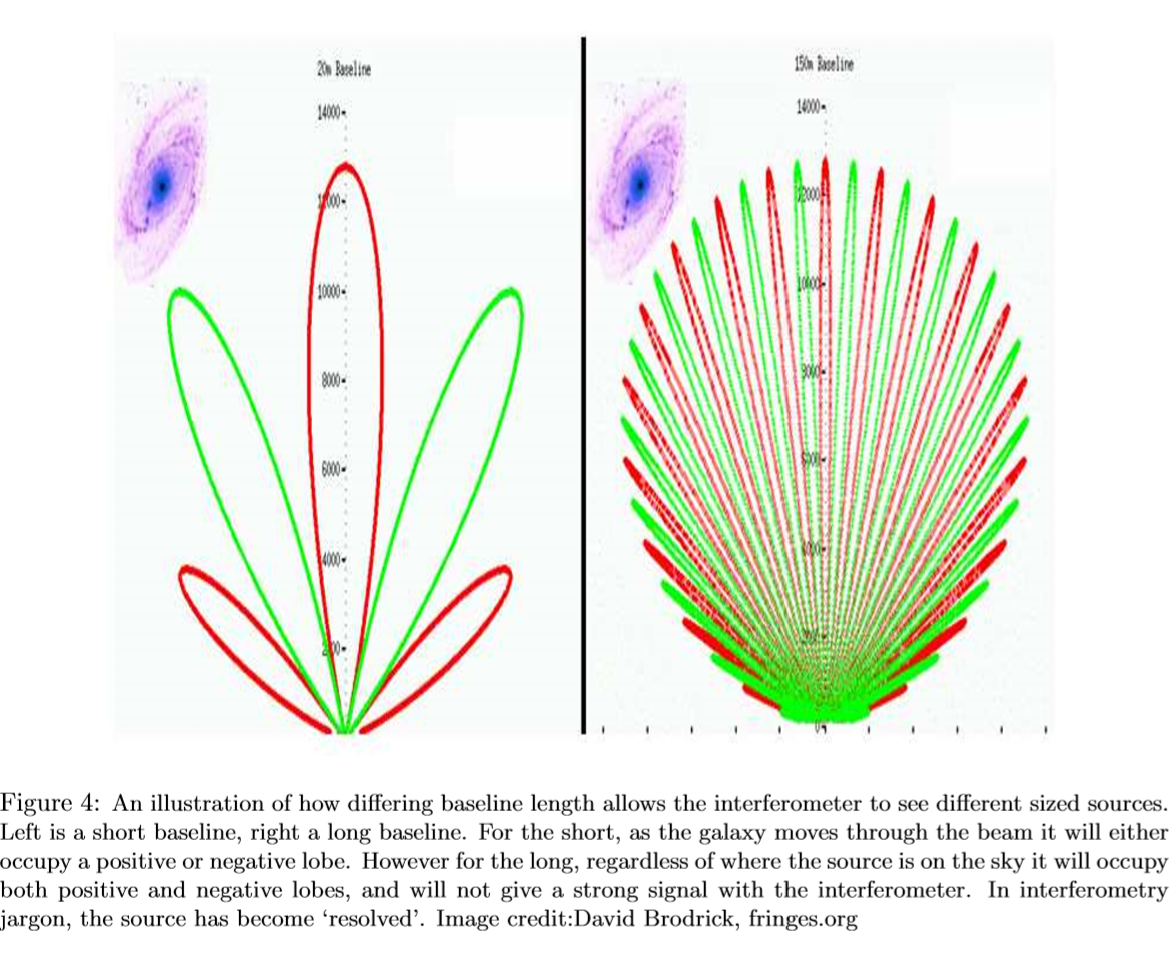
\includegraphics[scale=1]{loshortbaselines.png}
\end{figure}

\tbf{Fringe patterns and what we can find from it!}\\

One obvious application of this fringe pattern, is to measure accurate radio source positions, and indeed this is what the very first interferometers were used for. It is also straightforward to measure the size of a source, by extending the size of the baseline until a weaker signal is received. This occurs when the angular size of the source becomes comparable to the distance between positive and negative lobes (see figure \ref{baselines}), which we know. Observations of extragalactic sources are made very much easier by this property, in that Galactic diffuse radio emission is generally 'resolved out' allowing background sources to appear. Some further useful properties of an interferometer include the fact that any internal instrument noise common to one antenna will not be present in the cross correlated signal, as noise is generally not coherent.

\chapter{Introduction}
\section{Some Fundamentals of Radiation}
Radio waves are a form of electromagnetic (EM) radiation, just like visible light but at frequencies that are far too low for our eyes to detect.  The laws of physics require that EM radiation contains waves of both electric and magnetic fields and that in a vacuum these fields must be perpendicular to each other and to the direction of propagation of the waves. These electric and magnetic fields both oscillate in their own planes.
The two conjugate characteristics of radio waves are wavelength and frequency and for a single wave are related as:
\begin{equation}
\lambda \nu=c
\end{equation} 
Electromagnetic waves (radio or otherwise) are often created by a charged particle (usually an electron) when it undergoes an acceleration.  The reason that we usually consider the electron to do the radiating, and not the proton, is that the electron will undergo a much greater acceleration than the proton with the same magnitude of force because of its much smaller mass.  Light behaves both as a wave and a particle.  The oscillating electric and magnetic fields that we described earlier is the wave description of light.  We can also describe light by a particle we call the photon.  The photon has no mass, and its energy, E, is given by
\begin{equation}
E=h \nu =\frac{hc}{\lambda}
\end{equation}
\subsection{The Radio Window}
 The radio window, as it can be called, ranges in frequency from 10 MHz $(1\times 10^7 Hz)$ up to 300 GHz $(3\times 10^{11} Hz)$, or in wavelengths from 30 m down to 1 mm.  The energies of radio photons range from about $10^{-19}$ to $10^{-15}$ ergs (i.e., very tiny!!!).  The boundaries of the radio window are due to atmospheric and ionospheric processes.\\
\textbf{What happens at frequencies higher than the lower limit and higher than the higher limit of the radio band?}\\
At low frequencies (below about 10 MHz) free electrons in the ionosphere easily absorb and/or reflect radiation.  Frequencies below this can be generated and transmitted on Earth, but they can't escape through  the ionosphere. And likewise, waves with frequencies less than 10 MHz arriving from space cannot penetrate the ionosphere to reach ground-based radio telescopes.  Frequencies below about 10 MHz must be observed from space-based radio telescopes.  
 
At the high frequency boundary, absorption by H2O and O2 in our atmosphere blocks the radiation from space.  An especially unfortunate aspect of this is that these and many other molecules are abundant in space and so it is of scientific interest to observe at these higher frequencies to probe the emission and absorption by these molecules in space (such as in star formation regions).   Radio observatories that operate at mm wavelengths, therefore, are desirable and must be located at high altitude, dry locations (e.g. on mountain tops). 

\subsection{Spectroscopy} 
The radio-frequency spectrum appears to the user as a graph of intensity or flux density (i.e., the amount of radiation) vs. frequency or wavelength, as is often the case now for optical spectra taken with modern digital detectors.\\
There are three general types of spectra, as described by Kirchhoff’s rules. These are given as:
\begin{itemize}
\item \textbf{Continuous Spectra:} When a radiation source emits at all frequencies over a range without breaks, the spectrum is called a continuous spectrum and the emitting object is called a continuum source.  A classic example of a continuum source is an incandescent lamp. A plot of a continuous spectrum, for example, will show intensities over a broad range of frequencies, although the intensity of the emission can vary significantly. 
\item \textbf{ Bright Line or  Emission Line Spectra:} When a radiating object emits radiation only at some very specific frequencies, or wavelengths, the spectrum contains a set of discrete bright lines. These lines of light are called emission lines.  The reason that a light source would emit only at some very specific frequencies is due to the quantum physics of atomic and molecular structure.  An atom or molecule can be in an excited energy state and then spontaneously drop to a lower energy state.  To conserve energy, it gives off a photon that carries the exact amount of energy that the atom or molecule loses.  However, due to the laws of quantum mechanics, the internal energy levels of atoms and molecules are restricted to a set of discrete values. Thus, changes in energy (and hence the emitted photon energy or frequency) can only have certain specific values.   
 
\item \textbf{ Dark Line or Absorption Line Spectra:} A more complicated and interesting case arises when the radiation from an intense continuum source passes through a cool, transparent gas of atoms or molecules.  Some of the atoms or molecules in the gas can absorb photons from the continuum to raise them into a higher allowed energy level.  The photons that they absorb must have exactly the same amount of energy that the atom or molecule gains, and so only the photons of certain, specific frequencies will be removed from the continuum.  To an observer stationed beyond the cool gas, the spectrum will show the continuous spectrum of the background source with the radiation at these specific frequencies appearing darkened, thus the dark line nomenclature. 
\end{itemize}
\section{The Sky Coordinate System} 
\subsection{Right Ascension and Declination}
So, picture a globe of the sky, which is called the celestial sphere, with a globe of the Earth at its center.  Figure \ref{radec} should help with this visualization.  Extensions of the lines of longitude on the Earth produce similar lines on the sky, which we call lines of Right Ascension, often abbreviated either as RA or with the Greek letter $\alpha$.  Extensions of the lines of latitude make lines on the sky called declination, abbreviated either as Dec or $\delta$.  Since the apparent rotation of the sky is actually due to the rotation of the Earth, the poles of the celestial sphere are the points directly overhead the poles on the Earth.  \textbf{The sky, then, appears to rotate like a sphere about an axis running through it from the north celestial pole to the south celestial pole. }

\begin{figure}\label{radec}
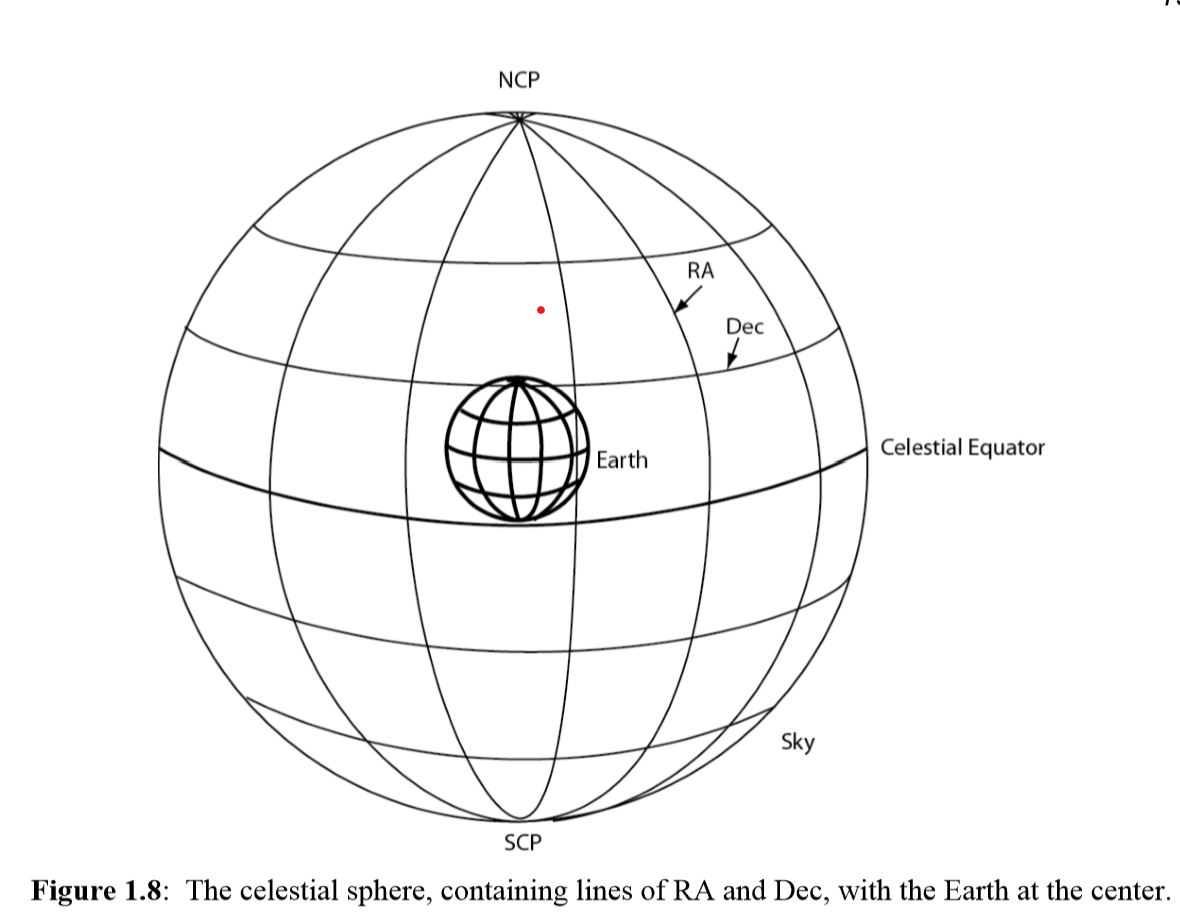
\includegraphics[width=\linewidth]{radec.png}
\caption{ The celestial sphere, containing lines of RA and Dec, with the Earth at the center. }
\end{figure}

The details of the sky coordinate system, though, are a bit more complicated because of the rotation of the Earth.  This rotation produces a constant relative motion between the lines of longitude and right ascension.  Since this doesn't happen with the lines of latitude and declination, declination is easier to handle, and so we'll discuss it first.   \\
It is natural to choose the $0^\circ$-line of declination to be the exact extension of the $0^\circ$-line of latitude.  Just as we call the $0^\circ$-line of latitude on the Earth the equator, we denote the $0^\circ$-line of declination on the sky as the celestial equator.  Then, the extension of the $10^\circ$-line of latitude to the sky points to the $10^\circ$-line of declination; likewise for the $20^\circ$ line, the $-10^\circ$ line, and so forth.  If you are standing at a latitude of $+45^\circ$, for example, and you point at the spot straight overhead, you will be pointing at a spot on the sky of declination $+45^\circ$. \\
Now let's consider the lines of RA; remember that they are complicated by the Earth's rotation.  If at some moment in time we define the $0$-line of RA to be the extension of the $0^\circ$-line of longitude, a minute later these lines will be shifted and, as the Earth rotates, they will continue to shift relative to each other.  Of course, we want the lines of RA to be useful for defining the position of an object on the sky.  So, we need the lines of RA to be fixed relative to the stars, not the Earth.  What astronomers have chosen to do is to pick noon on the first day of Spring (approximately March 21) as the moment in time when the $0$-line of RA aligns with the $0^\circ$-line of longitude (the latter passing through Greenwich, England).  And then, through our knowledge of how the Earth rotates during the day, and how it moves around the Sun in its orbit throughout the year, we can figure out by how much the lines of RA are shifted from the lines of longitude at any given moment of time during the year.\\
The units of right ascension are not what you would probably guess.  Longitude and latitude are both given in degrees, and so it would be natural to expect the same with right ascension and declination; and declination is, in fact, given in units of degrees.  Right ascension, though, has units of time; this needs some explanation.  In short, using units of time for right ascension makes most calculations involving RA simpler, as will become apparent later. First, note that the Earth's longitudes don't behave like normal angles. In particular, the angular separation between adjacent longitude lines depends on the latitude where the separation is measured.  Between $0^\circ$ and $10^\circ$ longitude there is an angular separation, as seen from the center of the Earth, of $10^\circ$, but only for points on the equator.  Away from the equator, the angular separation between any two lines of longitude decreases with latitude and even becomes zero at the poles.  The same, of course, occurs with the lines of right ascension.  The angular separation between any two lines of right ascension is proportional to the cosine of the declination.  Now, units of time turn out to be convenient to use for RA because the displacement between RA lines and longitude lines is related to the rotation of the Earth.\\
The units of RA are set up as follows.  There are 24 hours of RA around the sky, and each hour is divided into 60 minutes of RA, and each minute contains 60 seconds of RA.  Keep in mind, though, that 'one second of RA' does not equal 'one second of arc'.  In fact, since there are 24 hours of RA around the sky and 360 degrees around a full circle, at the equator 1 hour of RA = $15^\circ$ of arc, and so 1 minute of RA = 15 minutes of arc and 1 second of RA = 15 seconds of arc at the equator.  Away from the equator, the general relation between the number seconds of RA and seconds of arc is given by 
\begin{equation}
\text{seconds of arc}=15\cos(\delta)\times \text{seconds of RA}
\end{equation}
where $\delta$ is the declination.\\
Another apparent oddity is that if you look at a map of the sky with North at the top then East is to the left side of the map.  This is not due to some strange choice made by astronomers.  This, in fact, is the same East as on maps of the ground.  The reason for the apparent difference is that you, the observer, are between the ground and the sky and look in opposite directions to see each one.  Try the following stretching exercise.  Bend over and face the ground with the top of your head pointed to North.  Stick your right arm out to point to the East.  Now, without moving your arm or your body, twist your head around $18^\circ$o to look at the sky. (OK, you can't physically do that … but you can imagine it.)  If your right arm is still pointed to the East and the top of your head is to the North, with your head turned around $180^\circ$ to look at the sky, what direction is East?  Answer: to the left.  As an additional oddity when you look at a map of the sky, RA increases to the left, which, at first, seems the reverse of what you would expect.  We'll explain the reason for this in a little bit. 
\subsection{Observer Centered Definitions}
We also need a system that describes the way a particular observer (or telescope) sees the sky at any particular moment in time.  So, we need definitions to describe an observer-centered coordinate system. 
\begin{itemize}
\item \textbf{Horizon:} This defines the limit of what parts of the sky you can see at any particular moment.  It is due to the ground and structures on the Earth blocking your view of the sky.  If the Earth were transparent, you could also view the sky below your feet by looking through the Earth.  Since the Earth is not transparent, you can't see this part of the sky, because it is below your horizon.   
\item \textbf{zenith:} This is the point in the sky directly overhead.  Since the sky rotates continuously, this point on the celestial sphere continually changes, unless you are standing on either the North or South Pole.   
\item \textbf{altitude or elevation:} These are synonyms for the angular height of an object above your horizon at any given moment.  When a star is on your horizon (so that it is either just rising or just setting) its altitude, or elevation, is $0^\circ$ and when it is directly overhead – at the zenith -- its altitude, or elevation, is $90^\circ$. Check out Fig. \ref{altel}
\begin{figure}\label{altel}
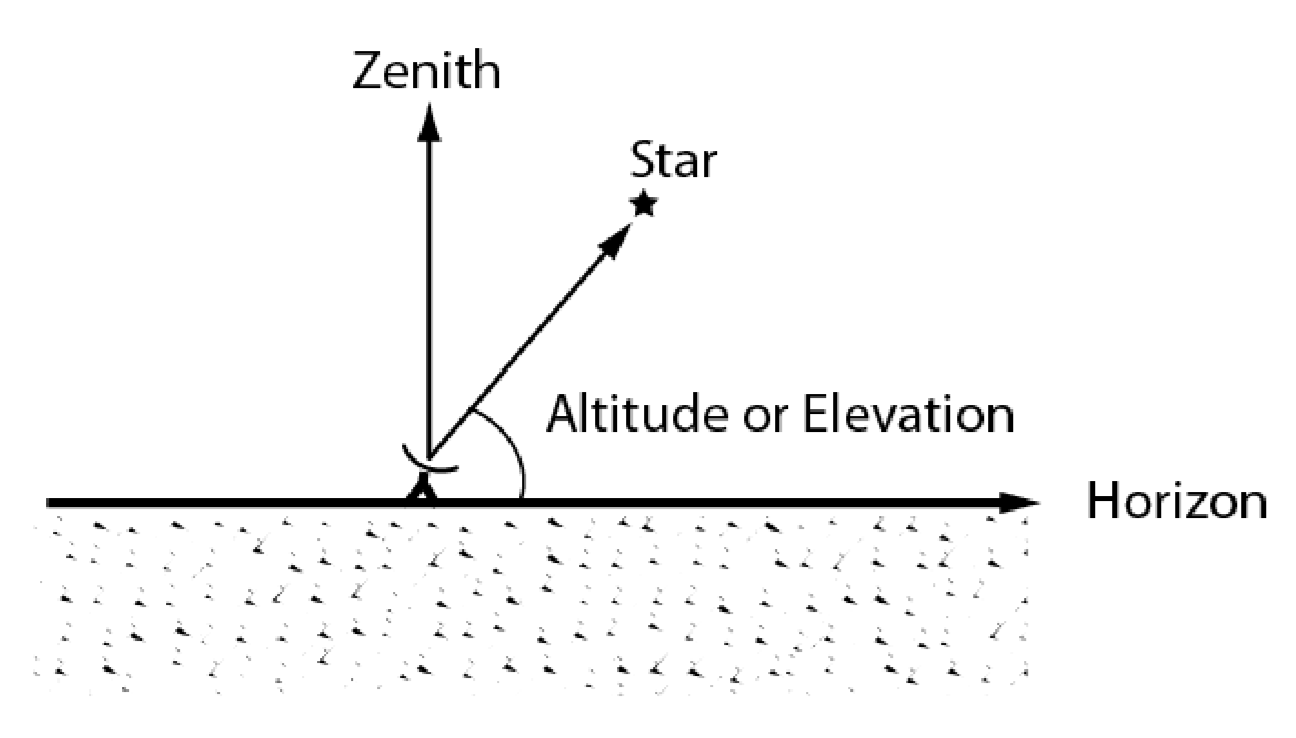
\includegraphics[width=\linewidth]{altel.png}
\caption{Schematic showing the relations between zenith, horizon, and altitude or elevation}
\end{figure}
\item \textbf{azimuth:}  This is the angular position perpendicular to the altitude, and defined as the angular position of an object along the horizon relative to due North.  If the object is located north of the zenith, its azimuth is $0^\circ$.  If it is south of the zenith, it has an azimuth of $180^\circ$.  An azimuth of $+90^\circ$ is due East and $270^\circ$ is due West. The angles of azimuth and their relation to the cardinal directions are shown in Figure \ref{figazo}. \textbf{ Note that azimuth and altitude make a pair of angles that completely define an object's position in the sky relative to the observer.  This last detail is important:  all observers will see the same RA and Dec for an astronomical object, but the altitude and azimuth for the object will be different for observers at different locations, and indeed, even for the same observer, at different times of the day. }

\begin{figure}\label{figazo}
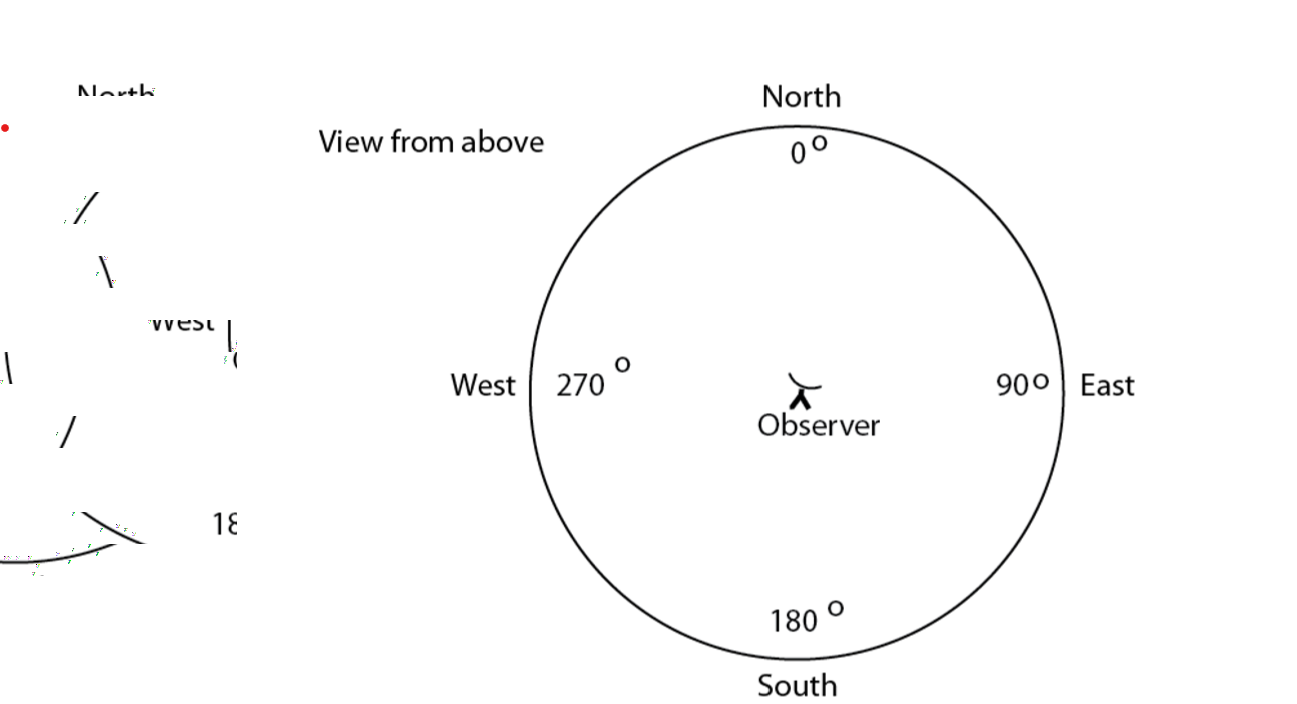
\includegraphics[width=\linewidth]{figazo.png}
\caption{ A view, from above, depicting azimuthal angles along with the cardinal directions around the horizon}
\end{figure}

\item \textbf{meridian:}  This is the line of RA that runs through your zenith.  Equivalently, it is the line in the sky that runs through both your zenith and the celestial poles.  Consider the following.  As the Earth rotates, you will see the stars move across the sky from East to West.  Consider, for a moment, just the stars that are at the same declination as your latitude; these are the stars that will pass directly overhead (i.e., through the zenith) on their trek westward.  The moment that one of these stars is at the zenith is when it is highest in the sky (i.e., when it reaches its maximum elevation).  Stars that are at different declinations will never pass directly overhead because the point directly overhead must have the same declination as your latitude (by definition of declination).  All stars, regardless of their declination, will be highest in the sky at the moment that they cross your meridian.  This is important because it is the best time to observe a particular object, and it also defines the mid-point of the time that an object is visible above the horizon (i.e., the moment in time halfway between rising and setting). 
\item \textbf{Transit (verb):}  means to pass through the meridian.  So, if your friend asks,"When does Mars transit?", he/she means at what time of day is Mars highest in the sky.  This is a typical question whose real meaning is, "When is the best time to observe Mars?"  Check your understanding: What is the azimuth of object when it transits?  Assuming that the object does not pass through the zenith, then its azimuth will be either 0 degrees or 180 degrees at transit. 
\item \textbf{Hour Angle(HA):}  An object's hour angle is the amount of time (in hours) since the object transited.  For example, if the object is currently at the meridian, its hour angle at that moment is 0.  If the object transited one hour ago, it has an HA of  +1 h, and if it will transit in two and a half hours then its hour angle is -2.5 h. 
\item Local Sidereal Time(LST):  This is defined as the RA of the meridian.  While you are observing, the computer will keep track of your LST.  This number is useful to help you keep track of what objects are transiting or when a particular object will transit.  You must know an object's RA (as given in a catalog) in order to observe it.  And, if you also know the LST, you can calculate the object's hour angle from: 
\begin{equation}
HA=LST-RA
\end{equation}
The name LST suggests that this is a measure of time. In fact, it is, but it runs faster than the time we normally use.  Consider the definition of the units of time that your watch or clock uses.  One hour on your watch is defined as 1/24th of a day, which is defined as the average time period between transits of the Sun (i.e., from noon to noon).  This method of measuring time is called solar time, because the Sun is used as the reference.  Sidereal time uses the celestial sphere (or stars, other than the Sun) in the same way.  One sidereal hour is 1/24th of the time period between transits of the same star.  Time on the local sidereal clock is given by the RA of the meridian.  For example, when the 12-hour line of RA is directly overhead, the local sidereal time is 12 hours.  You don't want to use sidereal time as a real measure of time, though, because one hour of sidereal time is not equal to one hour of solar time.  Each star rises 4 minutes earlier each day, meaning that a sidereal day is 4 minutes shorter than a solar day.  This is due to the Earth's orbit because of the Earth's motion about the Sun, in the time it takes to rotate once it has moved 1/365th of the way around its orbit, and so the direction of the Sun has moved slightly.  The Earth must rotate an additional four minutes for the Sun to reappear directly over the same place on the Earth.\\
An important point to remember is that a celestial object will transit when your LST is equal to the RA of the object.  The Galactic Center, for example, has a RA of about 18 h, so it is highest in the sky (and best observed) at an LST near 18 h.  Note, however, that because LST is slower' than solar time, the time of day when the Galactic Center transits will change throughout the year.  In the northern hemisphere, 18 h LST is in the daytime during the winter months, while it occurs at night-time during the summer months, gradually shifting by 4 minutes every day
\item \textbf{Universal Time(UT):} This is the solar time in Greenwich, England (i.e., the time on the clock where the longitude is 0o).  This is useful for marking the exact time of an observation or an event.  One doesn’t need to know, then, from what time zone the observation was made.  It defines a time that is the same for everyone on the Earth.  Universal Time is particularly useful for situations in which the different time zones can cause confusion.  Airlines, for example, actually schedule their flights using UT, but translate to local time for the customers.    \\
Now we can understand why hours, minutes, and seconds make a convenient choice of units for RA and why RA increases to the East.  Suppose you wish to observe an object whose RA is 12 hours and 10 minutes.  You look up at the sky and note that the object straight overhead has an RA of 4 hours and 10 minutes.  Now you can ask, “How long will it be before my desired object transits?”  The calculation you need to do is basically to treat the RA of the stars like the tick marks on a clock.  Currently, the LST is 4:10 and the question is really asking when will the LST be 12:10.  So the answer is simply 12:10 – 4:10 = 8 hours.  (This does not account for the minor difference between the movement of your clock, which is based on the Sun, and the movement in LST, which is based on the stars.)  Sources further to the East will transit at a later LST, hence their RA is larger; i.e., RA increases to the East.\\
\textbf{Check out Figure \ref{figall}!}
\begin{figure}\label{figall}
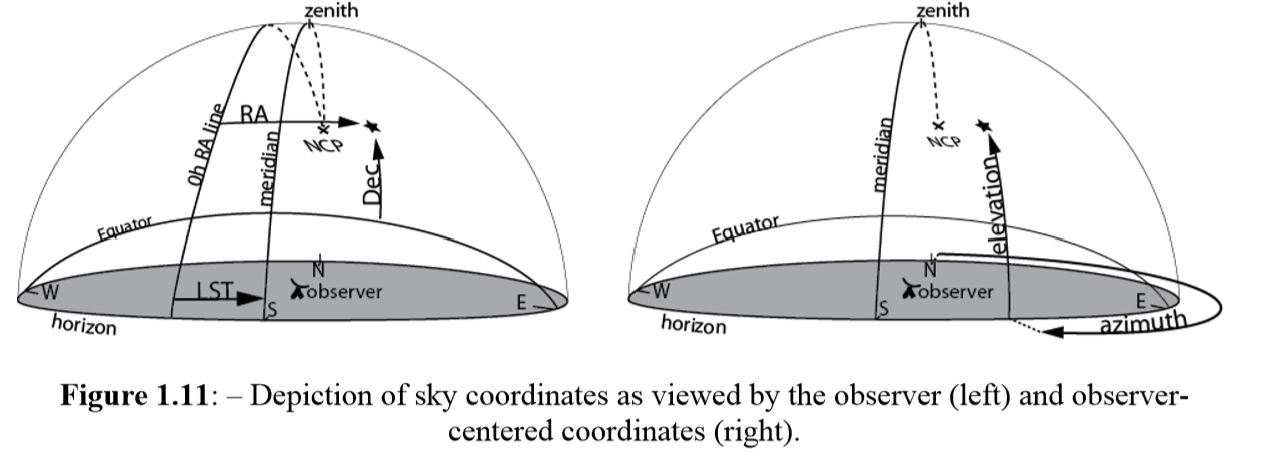
\includegraphics[width=\linewidth]{figall.png}
\caption{ Depiction of sky coordinates as viewed by the observer (left) and observer centered coordinates (right)}
\end{figure} 
\subsection{Apparent Size:}
In addition to an object's position, how we see it also involves its apparent size.  Our perception of size for distant objects is determined by the object's angular size, which is related to the object's linear size and distance.  However, we do not generally know an astronomical object's distance, so we often cannot know its linear size; but we can perceive its angular size. \\
In reality, objects in the sky appear to us as two-dimensional while angles, as we just discussed, are only one-dimensional.  We need, therefore, a two-dimensional description of angular size.  \\
This is called a solid angle, which we denote as $\Omega$.  To help gain an understanding of solid angle, consider a celestial object with a circular cross-sectional area small enough in angular diameter that $angular \;\; size(\theta)=\frac{diameter}{distance\;\;from \;\;observer}$ applies.  The calculation of the solid angle of the object, then, is essentially the same as calculating the geometric area of a circle.  (Hopefully, you remember that the area of a circle = $\pi R^2$ = $\pi(diameter/2)^2.)$  Since the angular diameter of the circular object is $\theta$(in radians), using our analogy between area and diameter of an object, its solid angle, $\Omega$, is

\begin{equation}
\Omega=\pi\cc{\frac{\theta}{2}}^2=(\pi/4)\theta^2
\end{equation} 
 
\end{itemize}
\section{Basic Structure Of Traditional Radio Telescope:}
\subsection{Parabolic Reflector}
 Since radio waves are easily reflected by metallic surfaces but not easily refracted, no radio telescopes are refractors (in contrast to visible-wavelength telescopes where lenses are sometimes used).  The radiation can then either be detected at the focal point of the dish or reflected back through the middle of the dish and focused and detected behind the dish. The former case is known as a prime focus telescope and the latter as a Cassegrain telescope.  \\
  Unlike visible light reflectors, radio dishes do not need highly polished surfaces.  Radio waves, being much longer than visible waves, can be reflected by a much less precise surface.  The general requirement for successful reflection of EM radiation is that irregularities in the reflecting surface be much smaller than the wavelength of the radiation.  We explain in Chapter 3 that a successful reflection is obtained when
\begin{equation}
\delta l <\lambda/20
\end{equation}
where $\delta l$ is the size of the surface irregularities of the reflector and $\lambda$ is the wavelength of light that we wish to reflect Surface irregularities of the reflector and $\lambda$ is the wavelength of light that we wish to reflect.  At longer radio wavelengths, in fact, the reflecting surface can even be a mesh, provided the holes in the mesh are sufficiently smaller than the wavelength of light to be reflected. 
\subsection{The Mount}
There are two types of telescope mounts, which in reality are the same but with different tilts.  All modern radio telescopes have altitude-azimuth or Alt-Az (also known as azimuth elevation or Az-El) mounts, meaning that the movement of the dish around one axis moves its pointing direction in altitude and movement around the other axis moves the pointing in azimuth. \\
The other type of mount, which is common for older and smaller visible-wavelength telescopes, is called an equatorial mount.  With an equatorial mount, the axes correspond to the sky coordinates: movement around one axis moves the telescope in RA and around the other axis moves it in declination.  An equatorial mount is really just an alt-az mount that is tilted so that the azimuth axis of the telescope points at the Celestial Pole rather than at the zenith. \\
\section{Radio Maps}
There are three common approaches to picturise the information obtained from the sky:
\begin{itemize}
\item \textbf{Contour maps:}The simplest way is with a contour map.  An example of a contour map is shown in Figure \ref{figcont}.  The contours are lines of constant intensity. An example of a contour map in which you may be familiar is a topographical map, in which the contours indicate the lines of constant elevation.   Many closely spaced contours indicate a steep slope in a topographical map.  In a similar way, a large number of closely spaced contours in an astronomical map indicates a region where the intensity is changing rapidly with the position. 
\begin{figure}\label{figcont}
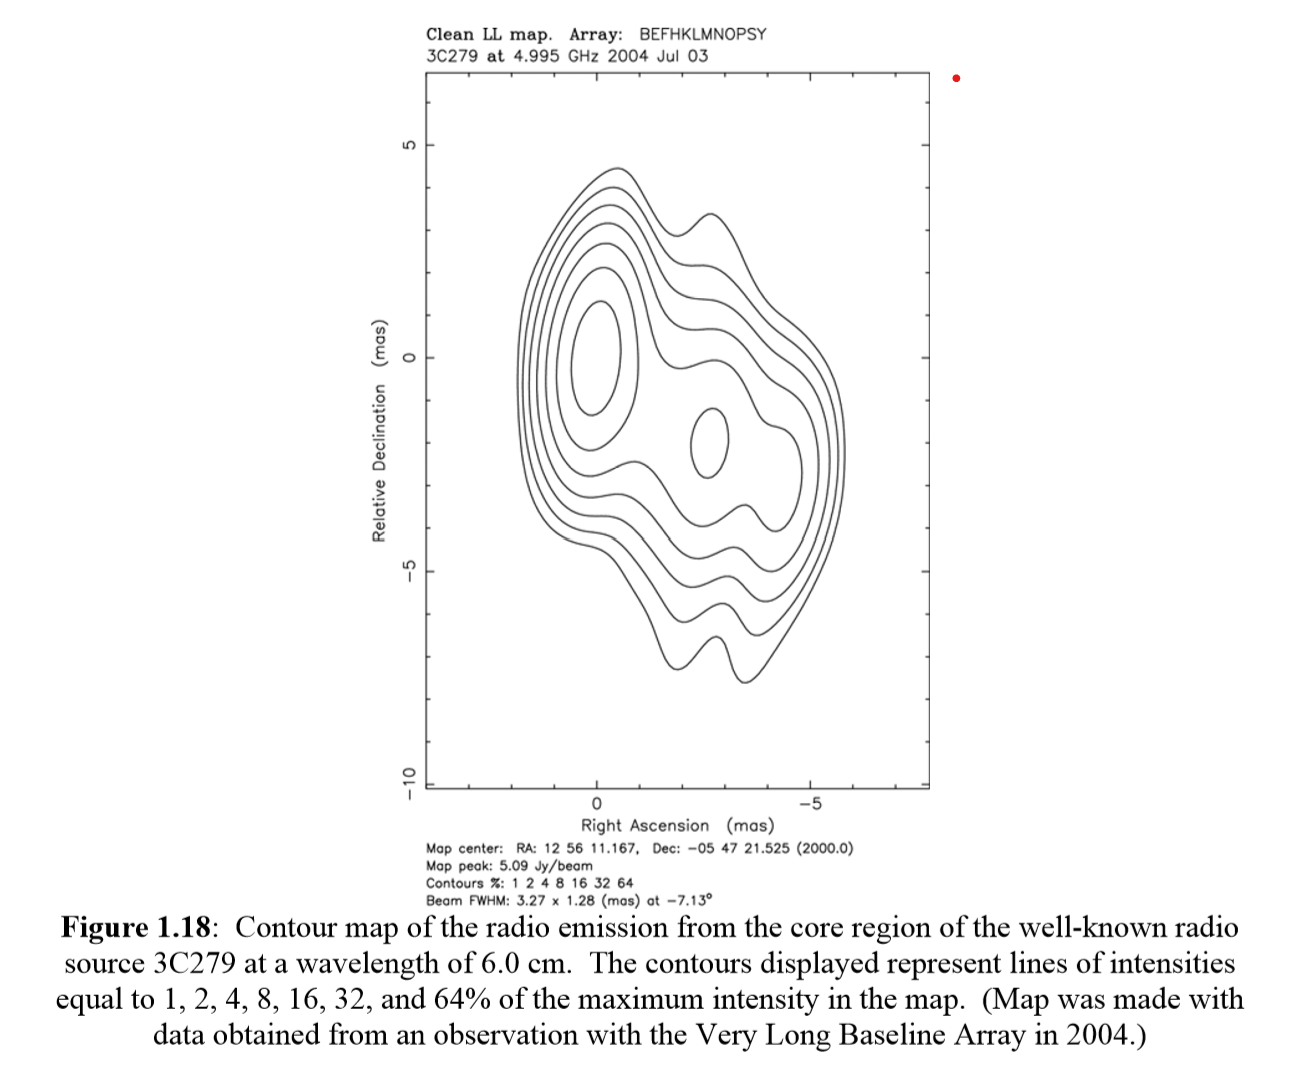
\includegraphics[width=\linewidth]{figcont.png}
\caption{ Contour map of the radio emission from the core region of the well-known radio source 3C279 at a wavelength of 6.0 cm.  The contours displayed represent lines of intensities equal to 1, 2, 4, 8, 16, 32, and $64\%$ of the maximum intensity in the map.}
\end{figure}
\item \textbf{Grey Scale Map:} A slightly more intuitive radio map is a grey scale map, in which no color is indicated, and the brightness variations in the source are directly indicated by the shades of grey, where black is the most intense and white is the least.  A grey scale map of the same source as in Figure \ref{figcont} is shown in Fig. \ref{figgrey}.  However, details in the structure are not revealed as well with a grey scale map as with a contour map, and so contour maps are often preferred for good analysis of the map.  (One should be careful, though, not to present too many contours, especially for a source with complex structure.  Overdoing contours with complex structure can sometimes make the image more confusing.)  It is very common, and quite pleasing, to present maps with both the grey scale and the contour maps overlaid as in Fig. \ref{figcorey}
\begin{figure}\label{figgrey}
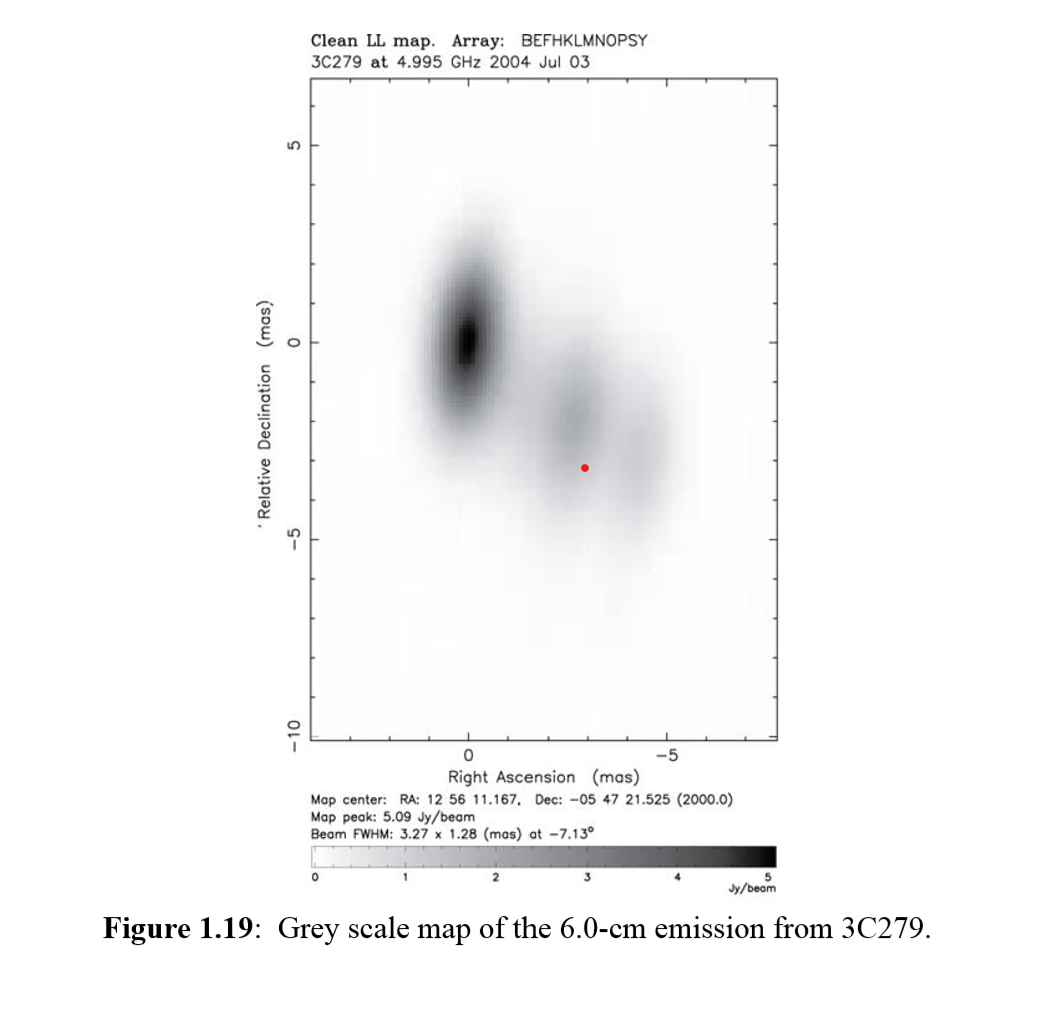
\includegraphics[scale=1]{figrey.png}
\caption{Grey scale map of the 6.0-cm emission from 3C279.}
\end{figure}
\begin{figure}\label{figcorey}
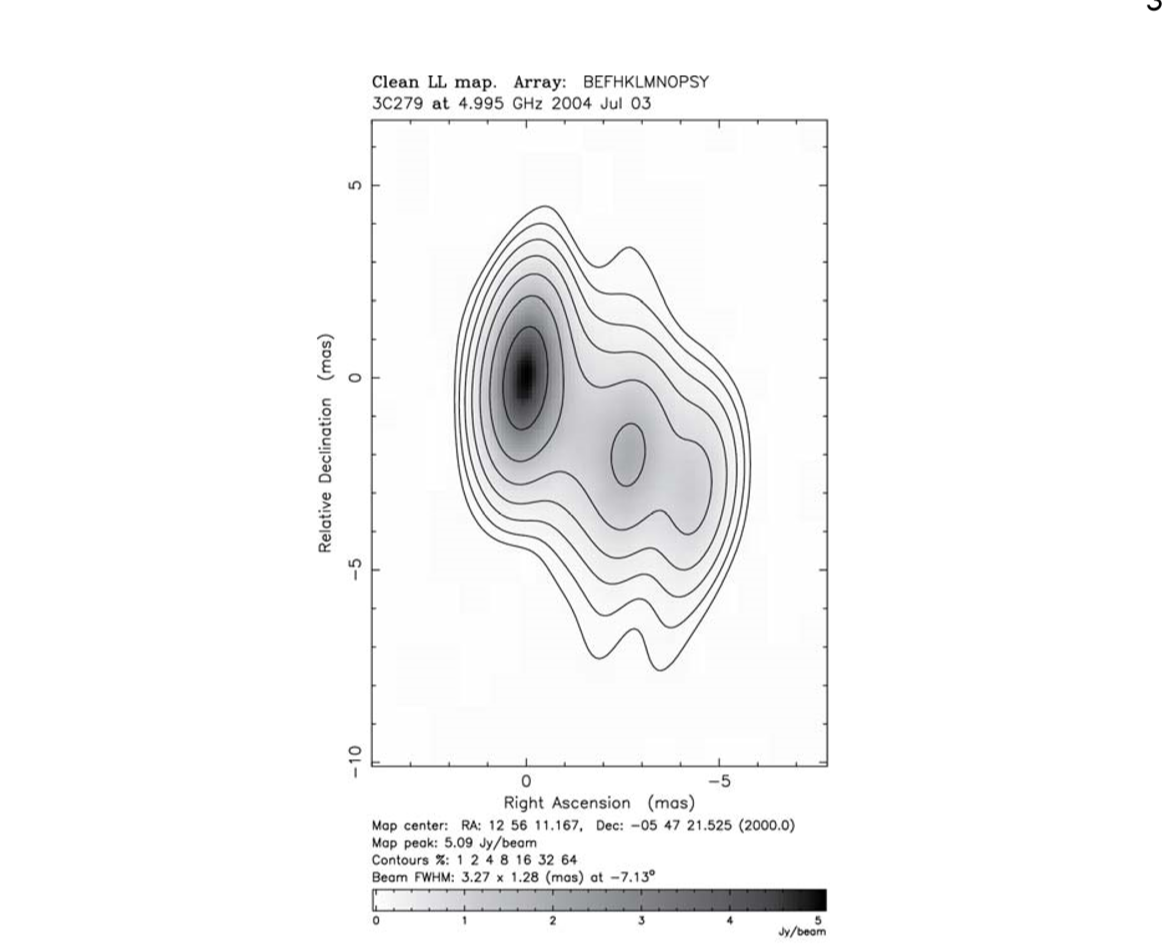
\includegraphics[scale=1]{figcorey.png}
\caption{contour map of same source overlaid over greyscale}
\end{figure}
\item \textbf{False color maps:}Many radio astronomers are quite fond of presenting false color maps, as shown in Figure \ref{figfal}, in which the color does not indicate different wavelengths but different levels of brightness. These images are usually accompanied with a color-wedge that indicates the relation between color and brightness. 
\begin{figure}\label{figfal}
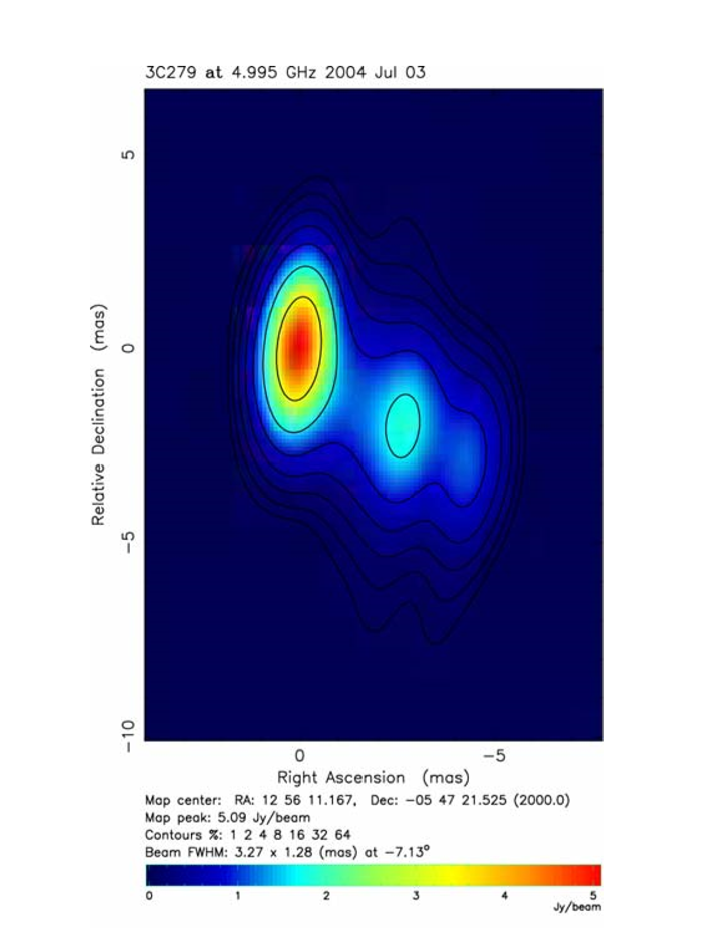
\includegraphics[scale=1]{figfal.png}
\caption{ False color map of the 6.0-cm emission from 3C279.  The color wedge at the bottom indicates the transfer function relating color and brightness.}
\end{figure}
 
\end{itemize}

\chapter{Introduction To Radiation Physics}
\section{Measures of the Amount Of Radiation}
\subsection{Total Energy Emitted}
One can describe a source's light output in terms of the total amount of energy emitted over a source's lifetime, at all frequencies, and in all directions.  This, however, is clearly not the kind of measurement that we can readily make.  Since one can make measurements only over a finite time period, one can only describe the amount of energy detected in that time period.  So that the measurement is independent of the time interval observed, a more useful quantity is luminosity or power, which is energy normalized by the time period. 
\subsection{luminosity(L)}
Luminosity or power is the rate at which energy is emitted.  Its S.I. units are J $s^{-1}$ or watts (1 W = 1 J $s^{-1}$) and $erg s^{-1}$ in cgs.  One calculates a source's luminosity or power by dividing the amount of energy emitted by the length of time over which the energy was emitted.  This yields the rate of emission.   \\
Luminosity, though, is not directly measurable because we don't detect all the radiation that was emitted by the source in any given second.  The vast majority of the radiation is emitted in directions other than towards our telescope.  This leads to our next quantity. 
\subsection{Flux(F)}
The radiation power that we detect depends on the size of our telescope -- the larger its cross sectional area, the more radiation will be detected -- so we again wish to normalize our measurement, this time, by dividing by the area of the telescope. This gives the measure of flux, i.e. the amount of light energy per unit time per unit area. The units of flux are J $s^{-1}$ $m^{-2}$ or W $m^{-2}$ (SI) and ergs $s-1$ $cm^{-2}$ (cgs).   \\
We can determine the relation between the detected flux and the luminosity of the source by calculating the fraction of the total emitted radiation that enters our telescope. If the radiation from the astronomical source is emitted isotropically (i.e., equally in all directions) and the source is at a distance d, then the luminosity is spread out over a spherical shell of radius d (see Figure \ref{figtele}).  The fraction that we detect is given by the ratio of the effective area of our telescope ($A_{eff}$) to the area of the entire spherical shell.  The surface area of the spherical shell is $4 \pi d^2$, so the power detected, P, is 
\begin{equation}
P=L\frac{A_{eff}}{4 \pi d^2}
\end{equation}
\begin{figure}
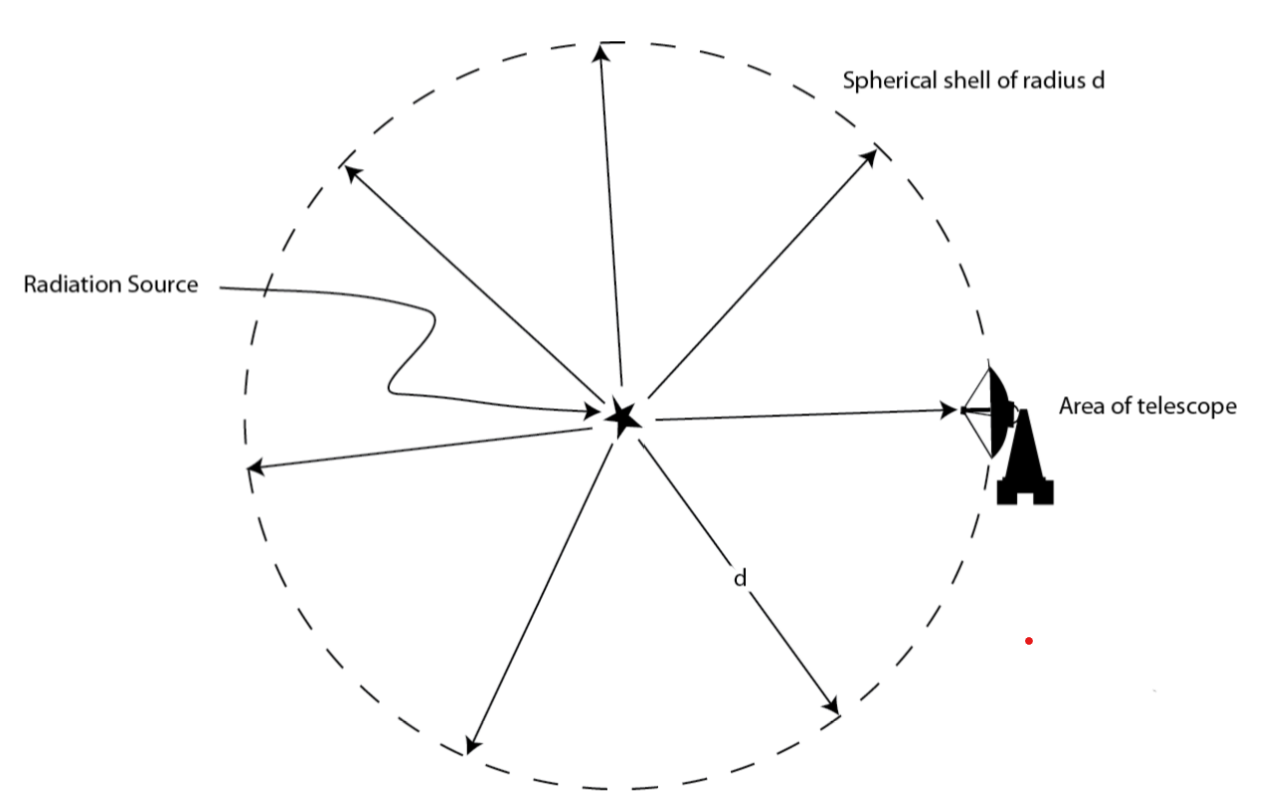
\includegraphics[width=\linewidth]{figtele.png}
\caption{ The radiation detected is the fraction of the total emitted that enters the small area of the telescope relative to the entire spherical shell of radius d. }
\end{figure}
 The radiation detected is the fraction of the total emitted that enters the small area of the telescope relative to the entire spherical shell of radius d. 
 \begin{equation}
 F=\frac{L}{4\pi d^2}
 \end{equation}
 \textbf{Flux, also, is not a truly measurable quantity because we can't measure the radiation emitted at all frequencies over the entire EM spectrum.  There is no detector in existence that can do that.  We can only detect the radiation emitted over the tiny fraction of the electromagnetic spectrum to which our detector is sensitive.}
 \subsection{Flux Density($F_\lambda$ or $F_\nu$)}
 Flux density is the flux per unit frequency in the observed spectral range and it equals the detected flux divided by the width in frequency of the observation.  So
 \begin{equation}
 F_\nu=\frac{F}{\Delta\nu}
 \end{equation}
 where $\Delta nu$ is the bandwidth or the range in frequency of the detected EM waves.  \textbf{The symbol $S_\nu$ is often used by radio astronomers to represent flux density per unit bandwidth}.  When working at visible wavelengths, astronomers tend to measure flux density in terms of wavelength rather than frequency, and so flux density is also often defined as flux per unit wavelength, 
 \begin{equation}
 F_\lambda=\frac{F}{\Delta \lambda}
 \end{equation}
we'll only use $F_\nu$ , the flux per unit frequency, since that is the standard approach in radio astronomy. We call this flux density because it describes the density of flux in spectrum space.  The mathematical relation between flux and flux density is 
\begin{equation}
F=\int F_\nu d\nu
\end{equation}
Flux density, at last, is a measurement that we can obtain directly and which all observers should agree upon, regardless of the telescope they use.  The telescope measures the amount of power it receives, and this depends on the collecting area and the bandwidth.  The flux density is the quantity about the source that we want to infer from these data.  The amount of power a telescope collects from a source of given flux density is given by 
\begin{equation}
P=F_\nu A_{eff} \Delta \nu
\end{equation}
  For astronomical sources at radio frequencies, the amount of energy we receive per unit time per unit area and per unit bandwidth is incredibly small, so both the SI and the cgs systems yield awkwardly small numbers for typical flux densities.  To avoid carrying around excessively negative powers of ten in our calculations, radio astronomers have defined a unit of flux density, named after the father of radio astronomy, Karl Jansky.  In units of the SI and cgs systems, a Jansky is defined as 
\begin{equation}
  1 \;\;Jy=10^{-26} W\; m^{-2}Hz^{-1}=10^{-23}\;\; ergs \;\; s^{-1}\;\;cm^{-2}\;\;Hz^{-1}
\end{equation}
This is a very important unit to radio astronomy; it is a good number to commit to memory – along with its units.   
\subsection{Intensity($I_\nu$ or $I_\lambda$)}
The last important quantity regarding the amount of radiation is also the most fundamental.  Intensity (or specific intensity), which is often referred to as surface brightness and sometimes just brightness, is the flux density per unit solid angle.\\
Intensity has units of $W\;Hz^{-1}m^{-2}sr^{-1}$(for $I_\nu$) or $W\;nm^{-1}\;Hz^{-1}m^{-2}sr^{-1}$(for $I_\lambda$)\\.
If you know the solid angular size of a source, you can calculate the average intensity of the source by dividing the measured flux density ($F_\nu$ ) by the solid angle of the source ($\Omega$).  A general expression of intensity, then, is given by
\begin{equation}
I_\nu=\frac{F_\nu}{\Omega}
\end{equation}
 Intensity is, in fact, the correct description of the quantity that your eye measures and your brain interprets.  When a light bulb appears especially bright (note the word that we use here: bright) your eye receives an especially large intensity of light.  Consider how the appearance of the light is affected when you surround the bulb with a much larger soft-light globe?  The total amount of light emitted is the same, but it comes from a larger surface, so the light seems less intense. \\
 There are several aspects of intensity that are important to know:
 \begin{itemize}
 \item Flux density, $F_\nu$ , doesn't distinguish between the directions that the photons come from or travel to, whereas $I_\nu$ does.  The directionality of the photons is important when studying the transfer of radiation through material, such as clouds of interstellar gas
 \item Intensity is independent of distance!  This is hard to believe at first, but is easy to show.  Intensity has two separate dependences on distance and they cancel with one another.  Intensity depends on flux density and solid angle, as
 \begin{eqnarray*}
 I_\nu=\frac{F_\nu}{\Omega}\\
 \text{where,}\\
 F_\nu \sim \frac{L}{4  \pi d^2 \Delta \nu}\\
 \text{and,}\\
 \Omega=\frac{\text{Cross-sectional area of source= A}}{d^2}\\
 I_\nu \sim \frac{F_\nu}{\Omega} \sim \frac{Ld^2}{4 \pi d^2 \Delta \nu A}
 \end{eqnarray*}
 and, the $d^2$ cancel
\begin{equation}
 I_\nu \sim \frac{L}{4 \pi \Delta \nu A}
\end{equation}
\item Intensity is a direct measure of the object's surface brightness, i.e., the amount of energy radiated per second per unit area of the surface per unit solid angle right at the surface.  Since intensity is independent of distance, the intensity one measures on Earth (or on Mars) will be the same as that measured right at the surface.   For example, consider two different objects--let's call them 'A' and 'B'--at the same distance with the same luminosity (L), flux (F), and flux density ($F_\nu$ ), but which have different intensities.  Let $I_\nu$ (A) > $I_\nu$ (B).  This can only occur when one of these sources is larger than the other so that $\Omega$(B)>$\Omega$(A).  Now consider what this means about the difference between the two sources.  For B to have the same flux density even though it has a larger surface, it must be less intense.  Intensity, we see, is directly related to the microscopic radiation processes of the object. If you measure a source's flux density and you can also measure the solid angle of the source (i.e., the source's size is large enough that you resolve its two-dimensional angular size) then you can get a direct handle on the microscopic radiation processes that produced the radiation.
\textbf{$1pc=3.096 \times10^{16}m$}.
 \end{itemize}
 
\subsection{Relation Between Intensity and the Electric and Magnetic Field Waves}
 the energy that we measure is contained in the electric and magnetic fields.  The energy flux of the radiation in terms of the fields is described by a quantity known as the Poynting vector, generally represented by S.  And, since the strength of the magnetic field in the radiation is directly proportional to the strength of the electric field, the energy flux in the radiation can be expressed in terms of just the electric field strength.
 \begin{equation}
 S=\frac{1}{2}c\epsilon_0E^2_0(SI)
 \end{equation}
 and
 \begin{equation}
 S=\frac{c}{8 \pi}E^2_0(cgs)
 \end{equation}
 where the amplitude of the electric field waves is represented by $E_0$.  (Note that a constant, $\epsilon_0$, the permittivity of free space, appears in the SI expression but not in the cgs expression.   This constant is not dimensionless; the definition of charge and electric field are quite different in the cgs system compared with the SI system, so changing systems is not as simple as just converting units.)
 
The important point to remember is that the intensity of the radiation is proportional to the square of the electric field in the waves, i.e. 
\begin{equation}
I_\nu \propto E^2
\end{equation}
 most radio telescope detectors produce a signal proportional to the square of the amplitude of the electric field so that the measured output is proportional to the power in the radiation. 
 
\section{Blackbody Radiation}
I have skipped 2.3 and 2.4 for a future reading.

\section{Coherent Radiation}
The radio-wavelength radiation emitted by an individual electron is undetectable by any radio telescope; the radiation we detect is the sum of many individual emission events by many individual electrons (or other charged particles).  Now, there are two very different ways that electromagnetic waves emitted by separate electrons can combine; and the way they add together makes a huge difference in how we treat the radiation mathematically and also in its physical properties.  \\
 let us imagine a single electron that is continuously oscillating at a fixed frequency, so that it continually emits electromagnetic waves at a single frequency or wavelength.  A chain of sine waves, then, propagates away from the electron.  Now imagine that after travelling some distance, this single chain of sine waves is joined by another chain of sine waves exactly in phase with it.  And, a little further along, it is joined by another wave chain, and then another, as depicted in Figure \ref{figele}
 
\begin{figure}\label{figele}
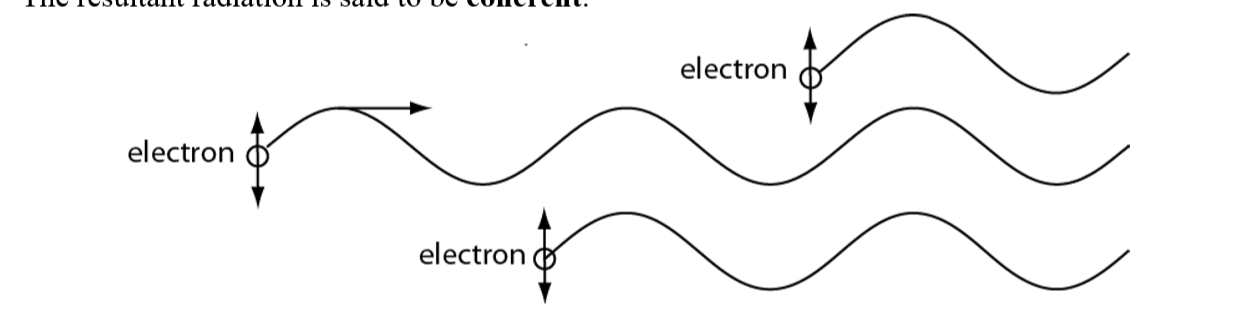
\includegraphics[width=\linewidth]{figele.png}
\caption{Schematic of the creation of coherent radiation.  An oscillating electron emits a chain of sine waves which is joined by another identical chain of sine waves with exactly the same phase, and then another wave is added, in phase with the first two}
\end{figure}
 Eventually, the initial wave chain has gathered many other identical wave chains, all in phase with each other.  Since all these wave chains are identical and with exactly the same phase, they add constructively, thereby amplifying the initial wave chain by a very large factor.  This is, basically, what happens in a laser and the result is that at any specific position in space at any given instant in time, one can assign a frequency, wavelength, and phase.  The resultant radiation is said to be coherent.   \\
In contrast, imagine the light created by adding the radiation emitted by many unrelated electrons. Each electron emits its radiation at some random time, independent of the radiation emitted by the other electrons.  This is what happens in an incandescent light bulb, for example, and in most astronomical sources.  The composite radiation in this case will involve numerous sine wave chains, but the frequencies, directions of travel, and phases of all the separate wave chains at any given location in space and at any given moment in time will be completely unrelated.  The resulting radiation, in this case, cannot be modeled by a single chain of sine waves.  The composite radiation in this case is called incoherent. \\
In mathematical terms, coherence of radiation is often defined as when radiation at any location in space and time has a specific phase.  However, the issue of coherence of radiation is actually more complex; its specific meaning depends on the context in which it is used.  There are different forms of coherence and varying degrees of coherence.  In the next section, we hope to convey a broader understanding of this phenomenon. \\
\textbf{I am skimming through these sections for now and would come back later.}\\
 In conclusion, with incoherent light, the total intensity equals the sum of the component intensities, whereas with coherent light, the total intensity grows as the square of the sum of the component intensities. \\
 Does this mean that we now have a problem with conservation of energy with coherent radiation?  Shouldn't the intensity of N beams simply be N times the intensity of one beam, whether they are combined coherently or incoherently?  Or do light beams added coherently magically have more energy than light beams added incoherently?  The answer is no; the intensities of the coherent and incoherent beams differ, but their total energies are the same.  Recall that intensity is flux of energy per unit solid angle per unit bandwidth.  The total flux in a beam is the intensity integrated over solid angle and over the bandwidth, i.e., 
 \begin{equation}
 F_\nu=\int I_\nu d\Omega d\nu
 \end{equation}
 The high intensity of a coherent light beam is only present over a small range of wavelengths and the beam is very narrow in solid angle.  Therefore, when the two intensities are integrated over frequency and solid angle they yield the same flux, or the same rate of energy flow.  
 
\section{Interference of Light}
skipped, but will come back when appropriate.
\section{Polarization}
 To describe this aspect, one talks of the polarization of the radiation. As an electromagnetic wave travels through vacuum, the direction of the wave propagation, of the electric field, and of the magnetic field must all be mutually perpendicular.  Consider electromagnetic waves travelling along the +z axis.  The oscillating electric field vector is perpendicular to this direction; we'll define these to be the $\pm y$ directions, and the magnetic field vector must be perpendicular to both of these, or the $\pm x$ directions. There are, however, an infinite number of directions that are perpendicular to the direction of travel and there is no law that determines in which of these directions the electric field must point - only that it be perpendicular to the magnetic field vector and to the direction of travel.  So, for our +z-traveling waves, the electric field vector can also oscillate in the $\pm x$ direction and the magnetic field vector then would oscillate in the $\pm y$ direction.  In fact, the electric field can oscillate in any other direction in the x y plane, while the magnetic field oscillates along the perpendicular line in the x-y plane.  Moreover, the electric field is not required to stay pointing in the same direction.  For example, the electric field could rotate around the z axis as the wave propagates; (the magnetic field would then also rotate so as to stay perpendicular to the electric field). \\
 
 \textbf{But does this question of direction at all matter?}
To see why the direction of the electric field matters, consider the effect that the different electromagnetic waves discussed above have on an electron along the path of the radiation.  The oscillating electric field will accelerate the electron, causing it to oscillate in the direction of the electric field.  (The magnetic field only accelerates electrons that are already moving and the resultant acceleration of electrons with typical velocities is insignificant in comparison to that produced by the electric field).  Now imagine that the electron is constrained to move only in the vertical direction (perhaps the electron is part of a very thin vertical wire antenna).  Then, a chain of electromagnetic waves whose electric field points in the horizontal direction cannot accelerate this electron at all and so these waves will pass by the electron with no effect, whereas electromagnetic waves whose electric field oscillates in the vertical direction will cause the electron to oscillate.  Even though these two sets of waves seem very similar in every way except for the direction in which the electric field vector points, they produce very different results.  We see, therefore, that the direction of the electric field vector is indeed important. \\
 we can treat any possible electric field as a resultant vector with two components lying in the x and y directions (see Figure \ref{figpol}).  For any individual electromagnetic wave chain, then, we need only to measure the electric field in the x direction and the electric field in the y direction, and then we've measured the vector's components, which is sufficient for a complete description of the whole vector.  These two base electric field measures we can call horizontal polarization and vertical polarization. 
 \begin{figure}\label{figpol}
 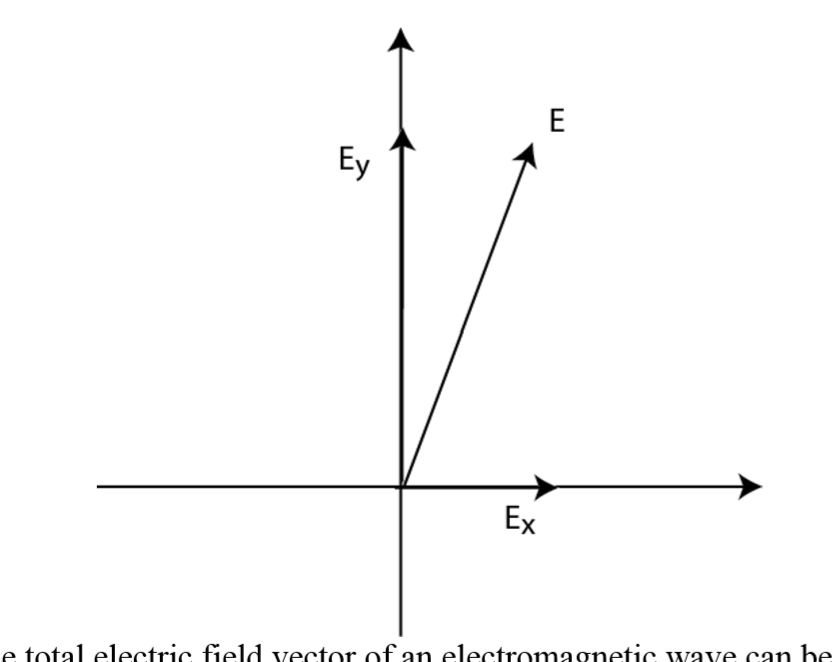
\includegraphics[width=\linewidth]{figpol.png}
 \caption{ The total electric field vector of an electromagnetic wave can be fully described by its components along the x and y axes. }
 \end{figure}
 
 An alternative, and equally correct approach, is to view two different circular polarizations—one rotating clockwise and the other rotating counterclockwise—as the base components for describing any polarization.  Just as a circularly polarized wave chain can be described as the sum of horizontally and vertically polarized wave chains, as we showed above, a linearly polarized wave chain can also be described by the sum of two oppositely rotating circularly polarized wave chains.  And, the phase difference between the circular polarizations will determine the orientation of the resultant linearly polarized wave chain.  Let's follow through with a particular example to see how this works.  Consider Figure 2.12 as we discuss this example.  Imagine two oppositely rotating circularly polarized wave chains in phase such that both their electric field vectors point upward (in the +y direction) at the same time.  Then, at this time, the sum, or the total electric field, will point upward and will equal the linear sum of the two component electric fields.  At this time, the resultant electric field has a maximum value.  As the two circularly polarized wave chains rotate in opposite directions, they will gain opposite valued x-components which will cancel, while their y-components decrease.  The resultant electric field, then, will still point in the +y direction, but will be smaller.  As the two waves continue to rotate in opposite directions, the total E field vector will continue to decrease and stay in the +y direction.  The total E field will continue to decrease until both of the rotating waves are horizontal, one pointing in the +x direction and one in the – x direction.  At this moment the two component E fields completely cancel out, and so the resultant E field vector is zero.  As the two waves continue to rotate they both gain -y components and the x components still cancel.  The sum will reach a maximum again when the two vectors are lined up along the – y axis.  We see, then, that the sum of these two opposite circularly polarized wave chains produces an oscillation only in the y direction, and so describes a linear polarization.  In similar ways, a wave chain of any polarization can be described either by a sum of two perpendicular linear polarization functions of time and phase or by a sum of two oppositely rotating circular polarization functions of time and phase.   
 
 
The two possible directions for circular polarizations are generally called left circular polarization and right circular polarization.  However, there is, unfortunately, an inconsistency in these definitions between different disciplines, which often causes a fair bit of confusion.  The reason for the inconsistency involves the different images one gets from different perspectives.  One who imagines the view of an approaching circularly polarized wave chain will define the rotation of the electric field in the opposite sense from one who imagines the view of a receding wave chain as seen from the source. 
Now, since the initial development of radio astronomy was accomplished by electrical engineers, especially those who are practiced in designing radio transmitters, the definitions and conventions used by radio astronomers to describe radio waves were established from the perspective of the source, viewing the radio waves traveling away.  The radio astronomer's definitions of right and left circular polarization (in the conventions established by the IAU (International Astronomy Union)), therefore, are the same as that given in the conventions of the IEEE (Institute of Electrical and Electronics Engineers).  In this convention, right circular polarization describes an electromagnetic wave whose electric field rotates clockwise as the wave comes out of the transmitter when viewing the wave from the transmitter and in the direction of propagation.  However, this means that the observer, who views the wave from the opposite direction, will see the electric field rotate counterclockwise.  So, in terms of the observation of a circularly polarized radio signal, right circular polarization means that the electric field vector, as it enters the antenna, is observed to turn counterclockwise with time.  Another, easy way to remember this is that a right circularly polarized wave obeys the right-hand rule in that when the thumb points in the direction of propagation, the curl of the fingers indicates the direction that the electric field turns. \\
There is confusion in these definitions because in most other fields of physics right and left circular polarization are defined in terms of the perspective of an approaching wave and so are given the opposite definitions from those used by radio astronomers.  Since radio astronomy is now considered a branch of physics there is a natural tendency to hold onto the definitions found in physics texts.  And, since radio astronomers naturally think of themselves as observing the radio waves as they enter the antenna, not creating them and sending them off to space, the physicist's definition, conceptually, makes more sense.  But, this is not the standard definition used in the field.  The lesson for us here is to remember the origin of the field that we're working in, which in this case is electrical engineering, and that the standard definitions in the field are influenced by the field's history. \\
In an actual observation of radiation from space, all the wave chains that enter your telescope are not going to have exactly the same polarization.  What you detect may have no net polarization, in which case it is called unpolarized radiation, or it may have a greater intensity in one polarization (horizontal vs. vertical, or left circular vs. right circular) in which case a percent polarization of the radiation is a useful measure.  \\
Analysis and discussion of polarized radiation is easier with the use of another set of polarization terms which we will now discuss in the next subsection.  This is the set of Stokes Parameters. \\
\subsection{Stokes Parameters:}
The first parameter, labeled 'I', is equal to the total intensity of all the radiation.  So, I equals the sum of the intensities of all orthogonal polarizations.  With the +z axis assigned to the direction of propagation of the wave, the electric field vector must be in the x-y plane, and so is described using only two orthogonal bases.  We have introduced two commonly used sets of independent bases (horizontal and vertical linear polarizations or left and right circular polarizations), so we can write I as
\begin{eqnarray}
I=I_x+I_y\\
or \;\; I=I_l+I_r\\
\end{eqnarray}
where $I_x$ and $I_y$ are the intensities of any two orthogonal linear polarizations and $I_l$ and $I_r$ are the intensities of the left circular and right circular polarizations. \\
The second parameter, labeled 'Q', is equal to the difference in the intensities of the two linear polarizations, so 
\begin{equation}
Q=I_x-I_y
\end{equation}
 The third parameter, 'U', is very similar to the second, but involves a rotation of the x and y axes by $45^\circ$.  If we call these shifted axes 'a' and 'b', shown in Figure \ref{figsto}, so that $I_a$ is the intensity of light that is linearly polarized along an axis halfway between the x and y axes and $I_b$ in the intensity of light polarized $90^\circ$ relative to a, then
 \begin{equation}
 U=I_a-I_b
 \end{equation}
\begin{figure}\label{figsto.ong}
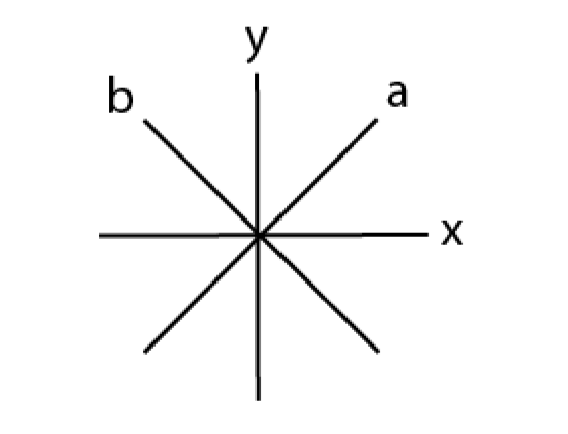
\includegraphics[scale=1]{figsto.png}
\caption{ Two sets of orthogonal axes for measuring polarization of radiation.  The x-y axes are used to calculate the Stokes Q and the a-b axes are used for the Stokes U.  }
\end{figure}  
The fourth parameter, 'V', is equal to the difference in the intensities of the left and right circular polarizations, so
\begin{equation}
V=I_R-I_L
\end{equation}
Stokes V, alone, is a measure of the amount of net circular polarization.\\
Q and U determine the amount of linear polarization.  To be more precise, the intensity of the net linear polarization, which we'll call L, is given by summing Q and U in quadrature, i.e., 
\begin{equation}
L=\sqrt{Q^2+U^2}
\end{equation}
One convenience of the Stokes Parameters should already be apparent; they provide a means of quantifying the linear and circular polarization intensities at the same time,  And, if the detected radiation has no net polarization, linear or circular, then
\begin{equation}
Q=U=V=0
\end{equation}
\textbf{The Case of Fractional Polarization:}\\
If there is no net circular polarization but there is non-zero linear polarization, then V = 0 and the fractional amount of linear polarization is given by L / I.  If there is no net linear polarization but a non-zero circular polarization, then Q = U = 0 and the fractional amount of circular polarization is $|V|$/ I.  If Q and/or U is non-zero and V is non-zero then the net polarization is elliptical.  The total fractional polarization can, in general, be expressed as  
\begin{equation}
\frac{\sqrt{Q^2+U^2+V^2}}{I}
\end{equation}
With elliptical polarization, the orientation angle of the major axis of the ellipse, relative to the x and y axes (as defined above), is called the polarization angle, and is often denoted by $\theta$, where $\theta$ is the angle starting from the +x axis and moving toward the +y axis.  The polarization angle is related to Q and U by 
\begin{equation}
\theta=\frac{1}{2}\tan^{-1}(U/Q)
\end{equation}
If there is a net linear polarization, the direction of the polarization in the x-y plane is the same as this angle (since a line is just a flattened ellipse).  Circular polarization, by its nature, has no major axis and so the polarization angle is is nonsensical.\\
You will also want to quantify the degree of ellipticity, which is commonly described by an angle denoted as $\beta$ in which tan$\beta$ is equal to the ratio of the amplitude of the electric field along the minor axis to that along the major axis of the ellipse, i.e., tan$\beta$ = Eminor/Emajor.  For pure circular polarization $\beta$ = $\pm \pi$/4 radians and for pure linear polarization $\beta$ = 0.  The parameter $\beta$ is determined from Stokes Parameters by 
\begin{equation}
\beta=\frac{1}{2}\tan^{-1}(V/Q)
\end{equation} 
Stokes Parameters are advantageous to use in describing polarization largely because they are all measures of intensity.  As such, there is no phase of the waves to worry about and they can easily be added, averaged, and manipulated algebraically.  In contrast, consider the difficulty in calculating the average position angle of linearly polarized radiation from a number of measurements, keeping in mind that polarization position angles that differ by $180^\circ$ represent the same radiation.  Imagine you had two measurements yielding polarization position angles of $1^\circ$ and $179^\circ$, which in terms of the physical orientation of the electric fields differ by only $2^\circ$.  When you algebraically average them you infer a position angle of $90^\circ$, which is orthogonal to the correct answer.  The proper approach is to keep track of the Stokes parameters, average their values, and then calculate the polarization angle
\chapter{Radio Telescopes}
A typical radio telescope consists of a primary reflector (or dish), feed, transmission line, and receiver. We note that radio telescopes operating at very long wavelengths (typically 1 meter or longer) can take a very different form.  Most radio telescopes are fully steerable, mounted on Alt-Az, (also called Az-El) mounts, and can point to any direction in the sky.  A computer controls the motion of the telescope and continuously translates the sky coordinates of an astronomical object into current altitude and azimuth positions. We will not discuss further the mechanics of how a radio telescope is mounted or moves. \\
\textbf{Some sections are skipped!}\\
The primary reflector serves two important functions. First, it collects and focuses the radiation from astronomical sources, making faint sources more detectable. The amount of radiation collected depends on the telescope's effective area ($A_{eff}$), which is closely related to the physical area of the primary reflector.  the power, P, of radiation collected from an astronomical source of flux density $F_\nu$  is given by
\begin{equation}
P=F_\nu A_{eff}\Delta \nu
\end{equation}
where the bandwidth, $\Delta \nu$, is the range of frequencies being detected.  The bandwidth, as we will discuss later, is determined by the receiver.  The larger the physical area of the reflector, the more power is collected from an astronomical source and the more readily faint sources can be detected.  As we will see, a number of factors impact the amount of radiation that enters the receiver and so the effective area of a radio telescope is always smaller than its geometrical area.  \\
The second function of the primary reflector is to provide directivity, which is a telescope's ability to differentiate the emission from objects that are close to each other, in angle on the sky.  When using a single radio telescope to make a map (as discussed in Chapter 4), the directivity determines the resolution in the map.  The directivity of a telescope depends, largely, on the diameter of the primary reflector and is governed by the principle of diffraction.  Diffraction, in fact, limits the directivity of all telescopes regardless of wavelength or frequency.  The directivity of a radio telescope is commonly described as the telescope's beam pattern, which is the topic of our next section.\\
\subsection{Beam Pattern}
The beam pattern is a measure of the sensitivity of the telescope to incoming radio signals as a function of angle on the sky.  This is similar to what optical astronomers often call the pointspread function. So the telescope is not only just sensitive to a point in space, its a non zero distribution of sensitivity over a a set of directions.  The term "beam pattern" derives from the idea of a beam of radio waves leaving a transmitting antenna.  Because the sensitivity pattern is the same, whether the antenna receives or transmits -- a principle known as the reciprocity theorem -- we are free to describe the pattern either way. \\
\textbf{ Ideally, we would like each feed in our telescope to collect radio signals from only one direction in the sky, so that when we point the telescope in a specific direction, the power detected through each feed corresponds to the radiation coming from only that spot on the sky.  Unfortunately, this is not possible due to the diffraction of light. Diffraction is a phenomenon of all types of waves, whether light waves, sound waves or water waves, that occurs when the waves pass through an aperture (or opening in which only a fraction of the wave front is not blocked).}\\
 The derivation in the appendix shows that with the case of a uniformly illuminated rectangular aperture, total destructive interference occurs for the sum of all the rays when the source is located $\lambda$/D radians from the central axis, where D is the distance across the aperture. \textbf{skipped some part} For a uniformly-illuminated circular aperture, like that of a typical optical telescope, the total collected power is zero when the source is 1.22($\lambda$/D) radians from the central axis. \\
  A sample plot of the sensitivity of a parabolic reflector as a function of angle is shown in Figure \ref{figairy}\\
 To understand these, return to the situation shown in where the phase difference is of order of $2\pi\frac{L\theta}{\lambda}$ where L be the distance between two interfering waves and $\theta$ is the angle when moved by sources causes the path difference resulting in interference of waves, and note that when $\theta$ = $\lambda$/L the phase difference is 2$\pi$ radians (one complete cycle) and so the waves from these two points are in phase again and add constructively.  Considering the entire aperture, though, one finds that there is only partial constructive interference.  The sensitivity of the telescope, therefore, has a small increase after it first reaches zero, as shown in Figure \ref{figairy}.  A telescope, then, can detect power from a source a good ways off-axis, although with much less sensitivity.  As the off-axis angle increases further, the response of the telescope goes through a series of peaks and valleys in which there is partial constructive and destructive interference.  These off-axis responses are called sidelobes and are undesirable as they can add confusion to observations.  For instance, we could detect as much power from a bright source located in one of these sidelobes as we detect for a faint source on-axis.  The central peak of the sensitivity pattern, in contrast, is often called the main beam. The telescope's sensitivity pattern, like that shown in Figure \ref{figairy}, is called the Airy pattern. \\


 
  
\begin{figure}\label{figairy}
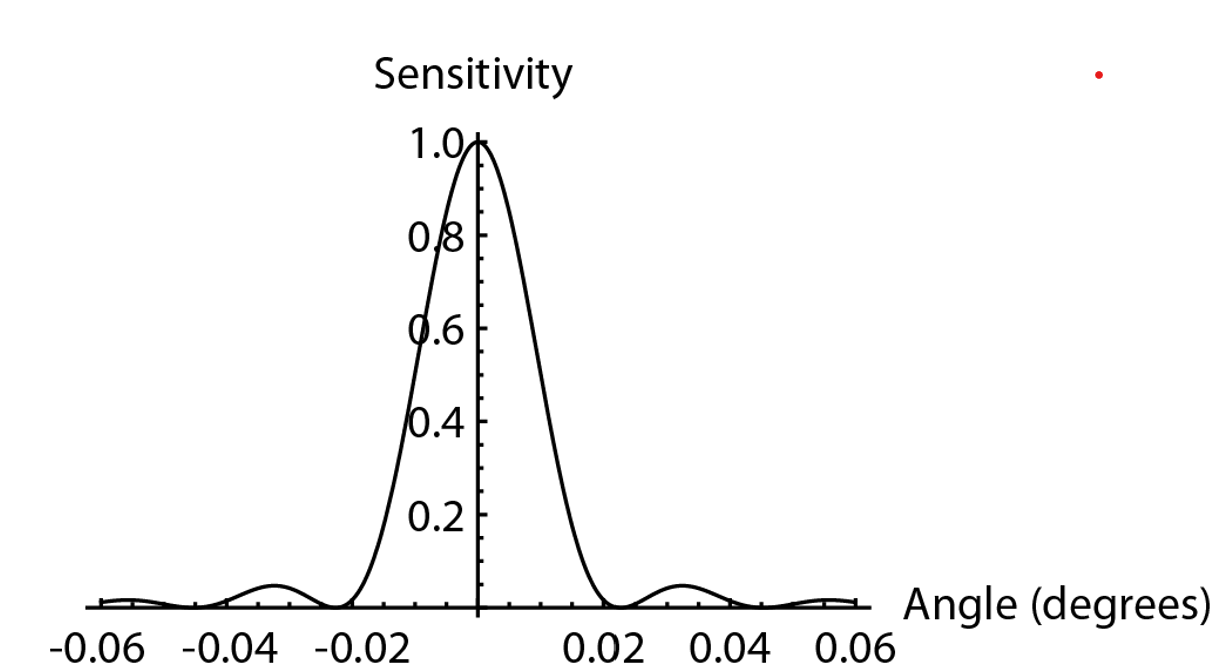
\includegraphics[width=\linewidth]{figairy.png}
\caption{ A typical profile of the relative sensitivity, or response pattern, of a radio telescope as a function of angle, $\theta$, relative to the telescope's central axis. The beam shown is for a uniformly-illuminated reflector with a diameter of 40 m observing at 1.4-cm wavelength. }
\end{figure}

\textbf{The width of the central peak of the Airy pattern is used to define the angular resolution of a singledish telescope.  By custom, we measure the angular width of this peak between the two points where the received power falls to one-half the on-axis value.  This angle we call the full width at half maximum (FWHM) of the main beam of the telescope.  }\\
The solid angle described by the main beam is considered to be the range over which the telescope can detect radio emission; that is, we can detect off-axis objects anywhere within this solid angle, albeit with reduced sensitivity, if they are located close to or inside the half power points.  Stronger sources may be detectable even further from the on-axis direction, but customarily we use the half power points to define the angular dimensions of the beam. \textbf{ This same angle defines the angular resolution of the telescope, because we cannot discern detailed structure of objects at smaller angular sizes.  This same angle defines the angular resolution of the telescope, because we cannot discern detailed structure of objects at smaller angular sizes. }\\
Our definition of the resolution angle, the FWHM of the main lobe of the antenna pattern, which is fairly standard in the radio astronomy community, is not the same quantity used in visible wavelength astronomy.  The canonical resolution angle of a visible-wavelength telescope is $\Delta \theta_{res}$=1.22 $\lambda$/D, which is the expression we gave above as the angle where the sensitivity pattern (of a circular, uniformly-illuminated aperture) first equals zero.  This is also defined as the radius of the Airy disk.  (Note that the plot in Figure \ref{figairy} is one-dimensional profile, while there are two angles on the sky, and so the central peak can be thought of as a disk, and the angle to the first null is its radius.)  The radius of the Airy disk, in fact, is larger than the FWHM of its central peak, which equals 1.02 $\lambda$/D.  (The visible-wavelength astronomy convention follows the Rayleigh Criterion, which defines the minimum angle of separation between two sources to be resolved as when the center of the Airy disk of one source is in the first null of the other.)\\
\textbf{Usually a small angular resolution is desirable, as it means that astronomical sources close together in angle on the sky can be distinguished or that fine angular detail can be discerned within a source.  Since the FWHM of the main lobe is inversely proportional to the diameter of the reflector, we have that }\\
\begin{center}
\textit{large diameter telescopes not only collect more power from an astronomical source, but also provide better angular resolution. }
\end{center}
\section{Noise, Noise Temperature and Antenna Temperature}

\textbf{How do we describe noise in observation?}\\
All the components in the receiver, especially the amplifiers, generate their own electrical signals that propagate through the receiver and are unrelated to the signal from the astronomical source. The power measured coming out of the detector, then, includes these extra signals, which interferes with our ability to detect and measure the power of the radiation from the astronomical source.  These extra signals are undesirable, but cannot be avoided.  We call this unwanted signal noise.  We need to be aware of the noise, and know how to account for it.  It is also desirable for the receiver to be designed so as to minimize the noise as much as possible.\\  
 \textbf{Concept of Equivalent Temperature!}\\
Characterizing noise signals generated in electrical circuits has, of course, always been of great interest in electronics.  Nyquist in 1928, for example, found that a resistor in the circuit will add electrical noise with a power per Hz that depends solely on the resistor's temperature.  For this reason, the electronic power in a circuit, in general, can be described in terms of an equivalent temperature, Tequiv, which equals the temperature of a resistor that would produce the same amount of power as the resistor.  Following this convention, radio astronomers also describe the power travelling in the transmission lines and receiver in terms of an equivalent temperature given by
\begin{equation}
T_{equiv}=\frac{P}{k \Delta\nu}
\end{equation}
where k is Boltzmann's constant and $\Delta \nu$ is the bandwidth of the radiation with power P. The above equation can also be viewed as using the Boltzmann constant (which has units of energy per Kelvin) as a conversion factor, to express energy (or power per Hz) in units of temperature. \\
\textbf{What is Antenna and Noise Temperature?}\\
Some of the detected power is due to the astronomical source, which was converted by the antenna to electronic power in the transmission line.  We call the equivalent temperature of the power that the antenna delivers to the transmission line, the antenna temperature, $T_A$. The far majority of the detected power, though, is due to noise from the receiver components.  We describe the total noise power by the noise temperature, $T_N$, and each component in the receiver is characterized by its own noise temperature. \\
\textbf{ We need, now, to discuss how the final power measured in the output of the receiver relates to the antenna temperature and the noise temperature of each of the components.  Keep in mind that both the source signals and the noise are affected by the amplification and losses that occur along the path through the receiver.  The equivalent temperature of the final power output, then, is not simply the sum of the equivalent temperatures of all the sources in the path. 
 }\\
 \textbf{The power measured by the receiver:}\\
 Let's first focus on the signal from the astronomical source and see how its power is affected by the processes in the receiver.  At each stage, the source signal is either amplified (when passing through an amplifier), or reduced by a loss (such as in a transmission line or in the mixer).  We can use the gain, G, defined by Equation $P_{out}/P_{in}$, for each step; when passing through an amplifier, G > 1, and when there is a loss, G < 1.  For example, if we assign a gain of G1 to the first element, which is the RF amplifier, then the power in the source signal after this stage is 
 \begin{equation*}
 P=G_1 k\Delta \nu T_A
 \end{equation*}
By the time the signal exits the detector, the power due to the radiation entering the antenna has been amplified by a net gain, G, and so 
\begin{equation}
P=Gk\nu T_A
\end{equation}
Note that the antenna temperature describes the power in the input radiation before any amplification.  Even though the amount of power increases when the signal is passed through an amplifier, the radiation is still described by the same equivalent temperature.  Therefore, regardless of the amount of amplification in the system, the input radiation power will still be described by the same antenna temperature.  Now, since we need to compare the noise power with the power from the astronomical source, we must describe both powers in the same way.  In particular, an amplifier's noise temperature is defined by the equivalent temperature of the noise power as if it were introduced at the input to the amplifier, and hence it is amplified along with the astronomical signal.  Imagine, for example, that the receiver contained only an amplifier of gain G1 and noise temperature TN1.  Then, the power output would be 
\begin{equation*}
P=G_1k \Delta \nu T_A +G_!k \Delta \nu T_{N1}=G_!k \Delta \nu (T_A+T_{N1})
\end{equation*}
Now, if we have two amplifiers in succession, the first characterized by $G_1$ and $T_{N1}$, and the second by $G_2$ and $T_{N2}$, then the noise power due to the first is amplified by a factor of G2 along with the noise produced by the second amplifier.  So the total noise power coming out of the second amplifier 
\begin{equation}
P_N=G_2G_1k \Delta\nu T_{N1} + G_2k \Delta\nu T_{N2}
\end{equation}
 the total gain in a succession of devices is just the product of the individual gains, so the total gain here is $G = G_1 G_2$.  Hence, we can define the total noise temperature ($T_N$) in this sequence of devices by 
 \begin{equation}
 P_N=G k \Delta\nu T_N
 \end{equation}
 
and so the total noise temperature relates to the individual noise temperatures as 
\begin{equation}\label{eqnoise}
T_N=T_{N1}+\frac{T_{N2}}{G_1}
\end{equation}
Note that the noise contribution of the second amplifier is reduced by the gain of the first amplifier. The total noise power, including all elements in the signal path, then, is obtained by considering the G and $T_N$ of all the elements in succession and applying the idea behind Equation \eqref{eqnoise}.  In general, for many elements in succession, we have: 
\begin{equation}
G=G_1G_2G_3\cdots
\end{equation}
and
\begin{equation}
T_N=T_{N1}+\frac{T_{N2}}{G_1}+\frac{T_{N3}}{G_1G_2}+\cdots
\end{equation}
\textbf{The total noise produced by all the components in the receiver is called the receiver noise temperature, $T_{rec}$. }\\
\textbf{Note that a lossy element, such as a mixer or transmission line, has G < 1, which, in effect, increases the contribution to the total noise temperature from all the components that come after it.}\\
\textbf{How could a loss cause an increase in the noise temperature? }\\
 Remember that the noise temperature describes the power before amplification (or loss), which makes it easier to compare the noise temperature and the antenna temperature.  The effect of a loss is to decrease the power in the source signal, and therefore any noise generated later in the signal path will appear larger, relative to the source signal, than if there had not been that loss, and so the value $T_N$ of these later elements must now be larger. \\
The RF amplifier, the first device the radiation enters immediately after the feed, therefore, is the most critical in determining the total noise temperature.  Since RF amplifiers usually have gains of at least a factor of 100 (or 20 dB), the contributions to the noise temperature of all other elements in the receiver and detector are reduced by at least a factor of 100.  A noisy mixer, for example, does not add that much to the total noise temperature, provided that its loss is not too great.  It is, therefore, extremely important that the RF amplifier has as much gain and as little noise as possible.\\
\textbf{What is the total power entering the detector?}\\
 Recall that the antenna temperature is defined before all the amplification.  Therefore, the total power entering the detector is given by 
 \begin{equation}
 P=Gk\Delta \nu (T_A+T_N)
 \end{equation}
 Considering the responsivity of the detector, we have the voltage out of the detector is
 \begin{equation}
 V=\alpha G k \Delta \nu (T_A+T_N)
 \end{equation}
 \textbf{For the majority of astronomical sources, and with most receivers, it is the case that $T_A$ << $T_N$ .  Therefore, even if we observe blank sky, the power out of the receiver is not zero because of the noise power. }\\
 \textbf{How do we solve for truncate the noise component when taking observations?}\\
  For these reasons, we cannot readily make total power measurements, but instead, we must make switched power measurements in which we measure the difference in voltage between when the telescope is aimed at the astronomical source, (called an on-source observation), and when it is aimed at blank sky (called an off-source observation). The latter 
 observation is made by pointing the telescope more than a beam width away from the source. Switched observations are discussed in more detail in the next chapter. \\
 \textbf{It is tempting to believe that the switched observations completely subtract off the noise power, and hence that noise is not really a concern. However, this is not the case.  The switched observations remove the offset in the measured power caused by the noise, but the fluctuations in the noise power still affect our measurement, and dominate our uncertainty in the antenna temperature.  It is these fluctuations that limit the sensitivity of a radio telescope to detect a faint astronomical source.}\\
 \subsubsection{The Statistics of Noise Signals}
 the variance is the mean square deviation from the average.  Following common convention, we will use $\sigma$ to indicate the standard deviation, and thus $\sigma^2$ as the variance. \textbf{\textit{The higher standard deviation, the more spread out the function is.}}.  And, therefore, for single-measurement experiments, the uncertainty equals the square root of the variance of that type of measurement.\\
 \textbf{What comprises fluctuations while measurement of power?}\\
   Now, when measuring the amount of power in electromagnetic radiation, the variance in the measure of that power depends on two effects.  Since the amount of power in the radiation is proportional to the number of photons arriving per second, the variance in power must relate to fluctuations in the arrival rate of the photons.  The power in the radiation is also proportional to E2 in the waves, and so the variance also depends on the fluctuations in the waves.  The former effect is a consequence of the particle aspect of light while the latter is often called the wave noise and is a purely classical effect.  When both effects are included in the statistics, the variance is found to have two terms; the variance due to fluctuations in the photon arrival rate depends on the number of photons and the wave noise depends on the number squared. \\
Or,
\begin{equation}\label{eqstat}
\sigma^2\propto n+n^2
\end{equation}
where,
\begin{equation*}
n=\frac{1}{\exp\cc{h\nu/kT}-1}
\end{equation*}
which (you hopefully recognized is the last factor in the Planck function) is proportional to the number of photons.  Note that the magnitude of n is less than one when h$\nu$>kT and greater than one when h$\nu$<kT.  Therefore, at higher frequencies, the first term in Equation 3.11 dominates and the uncertainty is proportional to the square root of the number of photons, i.e.
\begin{equation}
\sigma \propto \sqrt{n}
\end{equation}
while at lower frequencies, the second term dominates and the uncertainty is proportional to the number of photons,
\begin{equation}
\sigma \propto n
\end{equation}
If you are familiar with observations at visible frequencies, you may recall that one generally counts the number of photons – such as when measuring the brightness in the individual CCD pixels -- and that the uncertainty in that count is directly proportional to the square root of the count.  This is described by Poisson statistics, which describe the data when counting discrete objects.  At radio frequencies, though, when the photon energies are so low that the statistics falls into the wave regime, the uncertainty in the number of photons N is directly proportional to N.  Similarly, with the measured power we have 
\begin{equation}
\sigma_P \propto P_N
\end{equation}
\textbf{with any measurement involving random errors, the uncertainty in the measure decreases by averaging more values, by a factor equal to the square root of the number of measurements.  Similarly, by making the measurement for more seconds or by increasing the bandwidth, we make many independent measurements of the power.  In general, the number of independent measurements made over a time period of $\Delta t$ and bandwidth $\Delta \nu$ is given by $\Delta t \Delta \nu$.  Therefore,  in an observation with a bandwidth $\Delta \nu$ and integration time of $\Delta t$, the uncertainty in the power measured, $\sigma_P$, is given by }
\begin{equation}
\sigma_P=\frac{P_N}{\sqrt{\Delta t \Delta \nu}}
\end{equation}
The power measured is that of both the signal from the astronomical source and the total receiver noise power, however there may also be some additional unwanted noise contributions. Since the receiver noise power is usually much greater than the power from the astronomical source, it is the fluctuations of the noise power that limits the ability to detect a weak astronomical source.  For this reason, receiver noise, measured by the noise temperature, is a very important parameter to radio astronomers. The power measured is that of both the signal from the astronomical source and the total receiver noise power, however there may also be some additional unwanted noise contributions
\section{Very Low Frequency Radio Astronomy}
Since its inception, radio astronomy has tended toward higher observing frequencies.  Early on, this was an obvious way to achieve higher angular resolution, since $\theta_{resolution} \propto \lambda/D$.  As the field evolved, other reasons for observing at high frequencies also became apparent; particularly important was the fact that many molecules and interstellar dust emit radiation at shorter radio wavelengths.  These and other factors pushed radio astronomers to develop telescopes and receivers working at ever higher frequencies, and the trend is likely to continue.  As technology improves, the distinction between radio and the far infrared regimes is increasingly blurred, as radio techniques (in particular, coherent receivers) are being applied to even shorter wavelengths\\
This renaissance is mostly driven by scientific motivations, but as we shall see, there are important technological developments involved as well, with advances in computer technology being even more important than those in radio-frequency electronics.  For example, the first major radio telescope initiative of this century – the Square Kilometer Array – is based on the design concept known as ''Small-D, Large-N'', in which very many antennas (large N), each one of relatively small size (small D) work in concert, their individual signals being combined and processed by computers, which (currently) enjoy an exponential growth in capacity.
\textbf{skipped sections and subsections!}
\subsection{The Low Frequency Window}
The lower frequency limit for terrestrial radio astronomy is about 10 MHz.  This limit is determined by the plasma frequency of the ionosphere (see Vol. II), which is usually in the range of 3 to 5 MHz.  Below this cut-off frequency, radio waves arriving at the Earth are reflected outward by the ionosphere, thus never reaching radio telescopes on the surface.  The same effect occurs to low frequency radio waves generated on the Earth, reflecting these waves from the ionosphere back to the surface.  This is the principle behind long distance short wave radio communication.  Occasionally it is possible to observe as low as 3 – 5 MHz (when the free electron density in the ionosphere is unusually low) but reliable observing frequencies are somewhat higher, typically about 10 MHz.  The upper frequency limit for ''very low frequency'' is somewhat arbitrary.  The range from 300 MHz to about 600 MHz is where the transition from low frequency to high frequency methods and technology occurs.  We adopt 300 MHz ($\lambda$ = 1 m) as a reasonable value. 
\subsection{Antennas}
\textbf{skipped sections and subsections!}
\chapter{Single-Dish Radio Telescope Observations}
There are two principal – but greatly different - methods for making radio astronomy observations:  single-dish observations and observations made with multiple telescopes that are combined together using interferometric techniques.  In this chapter we give a thorough discussion of the basic considerations of radio observations made with a single telescope, generally referred to as single-dish observations.\\
The realtion  that relates the power collected by the telescope to the flux density, $F_\nu$, of the source radiation.
\begin{equation}
P=F_\nu A_{eff}\Delta \nu
\end{equation}
where $F_\nu$ is the flux density of the source, $A_{eff}$ is the effective area of the telescope and $\Delta \nu$ is the bandwidth over which the detection occurs
\section{Basic Measurements with single dish telescope}
\subsection{Switched Observations}
Imagine that you point a single-dish radio telescope at a known astronomical radio source and read the amount of power measured by the detector.  Is all of this measured power due to the astronomical radio source?  No.  As explained in Chapter 3, even when the telescope is pointed at a bright radio source, the power measured by the detector is dominated by noise -- primarily due to the electrical components in the receiver, but also, depending on the wavelength and the particulars of the observation, to background radiation from the sky and/or thermal radiation from the ground and the dish.  Therefore, the total detected power is actually a very poor measure of the power emitted by the radio source. \textbf{ In fact, the measure of a non-zero power, alone, is not proof that you have even detected the astronomical source.}\\
\textbf{To determine the amount of detected power due solely to the astronomical source, one must subtract off the power due to receiver noise and other sources of unwanted radiation.  This is a fundamental principle of single-dish radio observations -- all single-dish observations require the subtraction of the noise signal. }\\
\textbf{How do we solve this issue?}
This is accomplished by a process known as switching, in which the power is measured also when observing a nearby patch of sky that does not contain the astronomical source.  The power measurement when the telescope is pointed at the source is generally called the on observation, and the measured voltage is denoted as $V_{on}$, and the measurement when pointed away from the source is the off observation, with voltage equal to $V_{off}$. Another form of switching, called frequency switching, which can be used for spectral line observations is discussed in Section 4.4 .\\
\textbf{Let us see, how we remove this offset.}\\
 radio astronomers usually express the power measured from an astronomical source by its equivalent temperature called antenna temperature ($T_A$) while the noise power produced by the telescope receiver components is referred to as the noise temperature ($T_N$).   We lump all of this unwanted power together, and call it the system temperature ($T_{sys}$).  The voltage measured by the detector when the telescope is pointed at the source, or $V_{on}$,
 \begin{equation}
 V_{on}=\alpha Gk\Delta \nu (T_A+T_{sys})
 \end{equation}
where $\alpha$ is the responsivity of the detector (and has units of V/W), G is the dimensionless total receiver gain, k is Boltzmann's constant, and $\Delta \nu$ is the observing bandwidth (set by the bandpass filter).  Similarly, the voltage when pointed off-source, $V_{off}$,
\begin{equation}
V_{off}=\alpha G k \Delta\nu T_{sys}
\end{equation} 
Therefore, we can remove the system offset term by:
\begin{equation}
V_{on}-V_{off}=\alpha G k \Delta \nu T_A
\end{equation}
which is independent of the noise. So to find $T_A$, one then only needs to determine the conversion between temperature and voltage. \textbf{Instead of substituting in all the factors involved ($\alpha G k \Delta \nu$) this is accomplished by a calibration of the system temperature, which we explain in the next subsection. }\\

\textbf{Variation of gain of Radio Receiver and corresponding correction required?}\\
There is one other important issue about switching that we must address first.  The G in Equations presented above is the total gain of the radio receiver, which varies over time and can cause significant errors if not accounted for.  A variation in G of a few percent causes a deviation in the conversion from detected power, in volts, to antenna temperature, in Kelvins, in Equation $V_{on} $ by a few percent.  However, since the detected power from the source, $V_{on}-V_{off}$, is a tiny fraction of the total detected power $V_{on}$, a small variation in G, causing a small change in $V_{on}$, translates into a tremendous error in $V{on}-V{off}$, and could even result in a negative value for the calculated antenna temperature.\textbf{  To prevent gain variations from producing such enormous errors, the on and off observations must both be made regularly throughout the observation}


 




1.2.1, 1.2.3, 1.3.1, 1.3.2, 1.3.3,
1.3.7, 1.3.10, 1.3.12, 1.3.14 and 1.4.\\
\textbf{Michelson Interferometer}
\textbf{How does angular width of star determines the type of image obtained?}\\
 If the angular width \fn{Angular width of an object depends on how far we are from that object, the smaller angular width would mean, we are very far} of the star is small compared with the spacing in
between adjacent maxima, the image of the star is crossed by alternate dark and light bands, known as interference fringes. If, however, the width of the star\fn{example:this is true for maybe the sun} is comparable to the spacing between maxima, one can visualize the resulting image as being formed by the superposition of images from a series of points across the star. The maxima and minima of the fringes from different points do not coincide, and the fringe amplitude is attenuated. Fringe visibility is defined as 
\begin{equation}
\mbf{V}_M=\frac{I_{max}-I_{min}}{I_{max}+I_{min}} \leq 1
\end{equation}
Let $I(l,m)$ be the two-dimensional intensity of the star, or of a source in the case of a radio interferometer. $(l,m)$ are coordinates on the sky, with $l$ measured parallel to the aperture spacing vector and $m$ normal to it. The fringes provide resolution in a direction parallel to the aperture spacing only. In the orthogonal direction, the response is simply proportional to the intensity integrated over solid angle. Thus, the interferometer measures the intensity projected onto the $l$ direction, that is, the one dimensional profile $I_1(l)$ given by 
\begin{equation}
I_1(l,m)=\int I(l,m) dm
\end{equation}
 
\textbf{Michelson and Peas used mainly the circular disk model to interpret their observations and determined the stellar diameter by varying the aperture spacing of the interferometer to locate the first minimum in the visibility function.}

\section{two element radio interferometer}
\textbf{baseline:} the spacing between the antennas

\begin{\cbox}
\textbf{Problems in traditional interferometry?}\\
in addition to the signal from the source, the output of the receiver contains components from other sources of noise power such as the galactic background radiation, thermal noise from the ground picked up in the antenna side-lobes, and the noise generated in the amplifiers  of the receiver.\\
\textbf{For all except the few strongest cosmic sources, the component from the source is several orders of magnitude less than the total noise power in the receiver.}
\\
This noise offset is proportional to the receiver gain, which are difficult to eliminate.
\end{\cbox}

\textbf{What are the Consequences of this offset?}\\
The resulting drifts of the offsets in the output level degrade the detectability of weak sources and the accuracy of measurement of the fringes. 
\\
\textbf{Do we have any solution to this stupidity?}\\
\tit{Phase switching} by Ryle, helped to remove the unwanted components of the receiver output, leaving only the required fringe oscillations
\subsection*{Phase Switching Interferometer}
\textbf{What is the methodology behind Phase switching interferometer?}\\
If $V1$ and $V2$ represent the signal voltages from the two antennas, the output from the simple adding interferometer is proportional to $(V_1+V_2)^2$. In the phase-switching system, \textbf{the phase of one of the signals is periodically reversed}, so the output of the detector alternates between $(V_1+V_2)^2$ and $(V_1 - V_2)^2$. The frequency of the switching is a few tens of hertz, and a synchronous detector takes \textbf{the difference between the two output terms}, which is \textbf{proportional to $V_1V_2$}. Thus, the output of a phase-switching interferometer is \textbf{the time average of the product of the signal voltages}; that is, it is proportional to the cross-correlation of the two signals.\\
\textbf{What is a correlator?}\\
In Modern interferometry the circuitry responsible for multiplication and averaging of the two signals in called \textbf{the Correlator}.\\
\textbf{How does the phase switching affect the power term?}\\
In the traditional receiver the power was proportional to the squared sum of the two signals
\begin{eqnarray*}
P \propto \rr{V\sin (2 \pi \nu_0t)+V\sin (2 \pi \nu_0(t-\tau))}^2\\
\implies P= P_0\rr{1+\cos \cc{2 \pi \nu_0 \tau}}\\
\text{this power is power received by detector}\\
\text{where, $P_0$ is power generated by antenna alone (in absence of source)\fn{i do not understand this whole power equation, look into other books}}
\end{eqnarray*}
In case of phase-switching the cross term stays the constant term in power equation disappears, and the output only contains the fringes.
\\
\textbf{What is th significance of removal of constant term?}\\
The removal of the constant term greatly reduces the sensitivity to instrumental gain variation, and it becomes practicable to install amplifiers at the antennas to overcome attenuation in the transmission lines. This advance resulted in the use of longer antenna spacings and larger arrays. 

\subsection*{Optical Identifications and Calibration Sources}
\textbf{So you know, these discreet sources, how do you study them in optical?}\\
For the study of sources in optical, we would need high precision location of these sources. So, the principal method then in use for position measurement with interferometers was to determine the time of transit of the central fringe using an east west baseline, and also the frequency of the fringe oscillations, which is proportional to the cosine of the declination

The need for absolute calibration of the antennas and receiving system rapidly disappeared after a number of compact radio sources were identified with optical objects. Optical positions accurate to $\sim 1^{\prime \prime}$ could then be used, and observations of such sources enabled calibration of interferometer baseline parameters and fringe phases. 
\newpage
\section{Van Cittert-Zernike Theorem}
In this section we would learn about Van Cittert-Zernike Theorem. An optical term \textbf{Mutual Coherence} is used.\\
First, we would clear off the air around the Mutual Coherence function, For a field $E(t)$ measured at points 1 and 2, the \textbf{mutual coherence function} is given as
\begin{equation}
\Gamma_{12}(u,v,\tau)=\lim_{T\rightarrow\infty}\int^T_TE_1(t)E^\star(t-\tau)dt
\end{equation}
Here, u and v are expressed in wavelength and represent coordinates of spacing between two measurement point. \textbf{For zero time offset, $\Gamma_{12}(u,v,0) \equiv \mbf{V}(u,v)$; the complex visibility function for radio case}

Let us consider a system, which consists of an extended, quasi-monochromatic , incoherent source and let the mutual coherence of the radiation is measured at the point $P_1$ and $P_2$ in a plane normal to the direction of source.
\begin{figure}[h!]
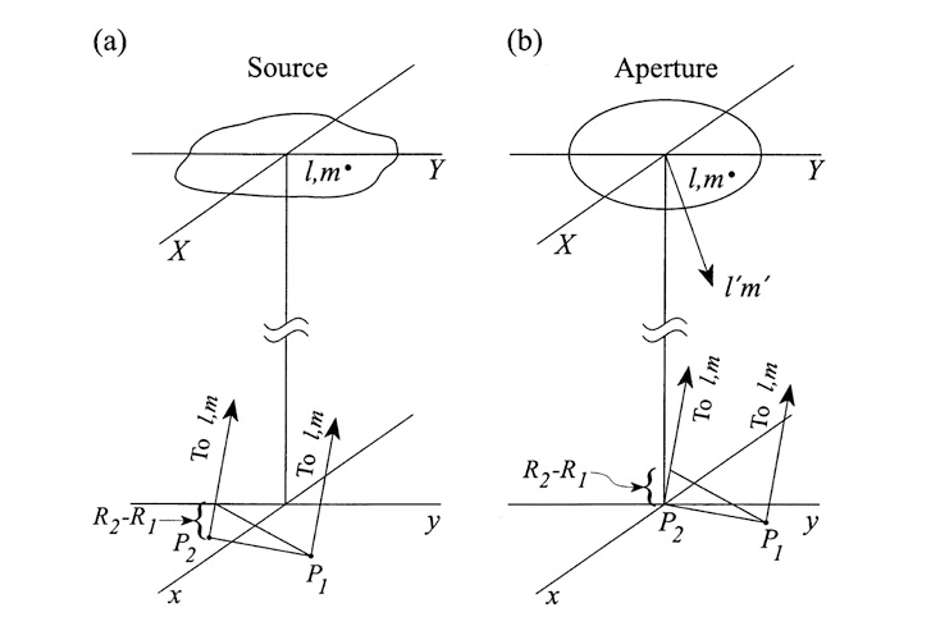
\includegraphics[width=\linewidth]{notesfig1.png}
\label{VCZ}
\end{figure}


The diagram (b), represents the same system , but with the source replaced \textbf{by an aperture of identical shape and size and illuminated from behind by a spatially coherent wavefront.}\\
Note point: 
\begin{itemize}
\item The distribution of the electric field amplitude over the aperture is proportional to the intensity distribution over the source.
\item Fraunhoffer diffraction pattern is observed in plane containing \textbf{$P_1$ and $P_2$} 
\item $P_2$ lies on the maximum of diffraction pattern, even though relative position for $P_1$ and $P_2$ is basically the same.
\end{itemize}

\textbf{VCZ} theory is based on the the fact that the behavior of both the mutual coherence and the Fraunhofer diffraction can be represented by similar Fourier transform relationships.
 
\subsection{Mutual Coherence of an Incoherent Source}
 
Now, consider the same system we mentioned above in Fig. \ref{VCZb}
\begin{itemize}
\item Consider source to be located in a distant plane given by (X,Y). 
\item Now, the radiated field is measured at points $P_1$ and $P_2$ in the (x,y) plane that is parallel to the source in the plane. \textbf{When we talk in case of radio, basically $P_1$ and $P_2$ refer to interferometer antenna locations.}
\item For, convinence to specify a point in (X,Y) plane, with respect to (x,y) we use direction cosines (l,m).
\end{itemize}
\begin{figure}[h!]
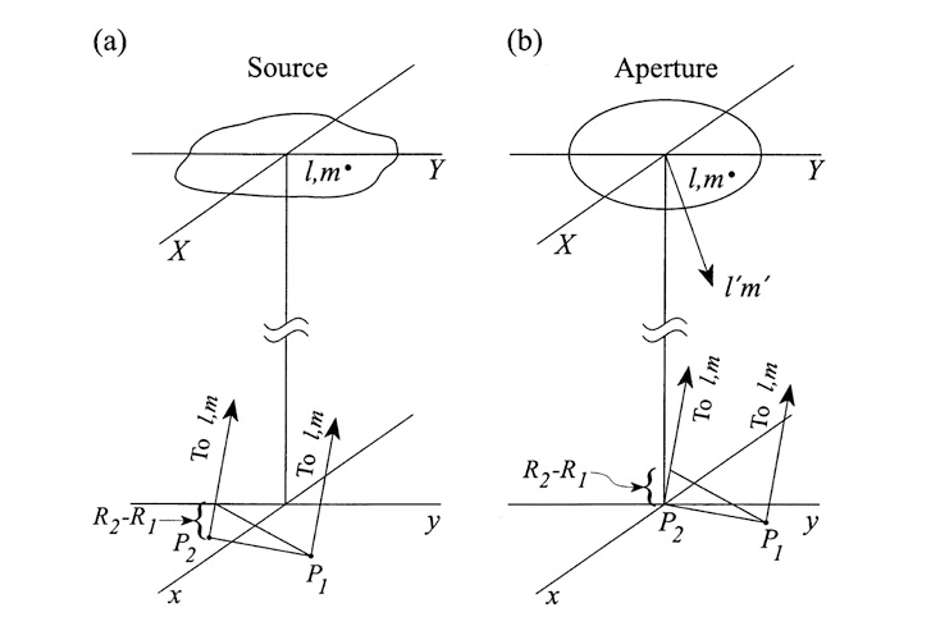
\includegraphics[width=\linewidth]{notesfig1.png}
\label{VCZb}
\end{figure}
Now, the fields at $P_1$ and $P_2$ resulting from a single element of source  is
\begin{equation}
E_1(l,m,t)=\varepsilon(l,m,t-\frac{R_1}{c})\frac{\exp[-j2\pi\nu(t-R_1/c)]}{R_1}
\end{equation}
and 
\begin{equation}
E_2(l,m,t)=\varepsilon(l,m,t-\frac{R_2}{c})\frac{\exp[-j2\pi\nu(t-R_2/c)]}{R_2}
\end{equation}
Here
\begin{itemize}
\item $\varepsilon(l,m,t)$ is the complex amplitude of the electric field at the source at element (l,m).
\item $R_1$ and $R_2$ are distances from the elememt from $P_1$ and $P_2$
\item Exponential term will represent the phase change in light traversing the paths from source to $P_1$ and $P_2$.
\end{itemize}
Now, the complex cross-correlation of the field voltages at $P_1$ and $P_2$ due to radiation from the element at (l,m) for the specific case of zero time offset is given as 
\begin{eqnarray*}
\aab{E_1(l,m,t)E^\star_2(l,m,t)}=\aab{\varepsilon(l,m,t-\frac{R_1}{c})\varepsilon^\star(l,m,t-\frac{R_2}{c})}\\
\times \frac{\exp{\rr{-j2\pi\nu(t-R_1/c)}}\exp{\rr{-j2\pi\nu(t-R_2/c)}}}{R_1R_2}
\end{eqnarray*}
\begin{equation}
=\aab{\varepsilon(l,m,t)\varepsilon^\star(l,m,t-\frac{R_2-R_1}{c})}\frac{\exp{\rr{j2\pi\nu((R_1-R_2)/c)}}}{R_1R_2}
\end{equation}
\begin{\cbox}
If the source is spatially incoherent , this means terms of form $\aab{E_p(l_p,m_p,t)E^\star_q(l_q,m_q,t)}$, where p and q refer to different elements of the source, is 0.
\end{\cbox}
\textbf{Simplification:}if the quantity $\frac{R_2-R_1}{c}$ is small compared with the reciprocal receiver bandwidth $\implies$ we can ignore, this term  in amplitude terms for $\varepsilon$.\\
Therefore the above equation for cross-correlation is reduced to:
\begin{equation}
\aab{\varepsilon(l,m,t)\varepsilon^\star(l,m,t)}\frac{\exp{\rr{j2\pi\nu((R_1-R_2)/c)}}}{R_1R_2}
\end{equation}
\begin{itemize}
\item $\aab{\varepsilon(l,m,t)\varepsilon^\star(l,m,t)}$ is a measure of \textbf{time-averaged intensity}, $I(l,m)$ of the source. 
\end{itemize}
So, now we found cross-correlation for one element and for finding mutual coherence function of fields at points $P_1$ and $P_2$, we integrate over the source, using $ds$ to represent an element of area within the $\cc{X,Y}$ plane:
\begin{equation}\label{croscor}
\Gamma_{12}(u,v,0)=\int_{source} I(l,m)\frac{\exp{\rr{j2\pi\nu((R_1-R_2)/c)}}}{R_1R_2}ds
\end{equation}
\textbf{Note:}Here, u and v are measured in wavelengths and are \tit{x and y components of spacing between the points $P_1$ and $P_2$}
.
\begin{itemize}
\item $R_1 \;\; \& \;\; R_2$ is the differential distance in the path lengths from (l,m) in the source to $P_1$ and $P_2$.
\item Coordinates for $P_1$ and $P_2$ are $(x_1,y_1)$ and $(x_2,y_2)$ respectively.
\item Hence, $u=(x_1-x_2)v/c$ and $u=(x_1-x_2)v/c$.
\item Now. $\implies (R_1-R_2)=(ul+vm)c/v$
\item now, as source is far away from $P_1$ and $P_2$, $R_1\simeq R_2 \simeq R $.
\item Here,R is the distance between (X,Y) and (x,y) origins.
\end{itemize}
Now if $ds=R^2dldm$ then \eqref{croscor} is given by:
\begin{equation}
\Gamma_{12}(u,v,0)=\int \int_{source} I(l,m){\exp{-j2\pi (ul+vm)}}dldm
\end{equation}

\textbf{Note:} as the integral outside boundary is zero, therefore we can extend to infinity.\\
\begin{\cbox}
And hence, the mutual coherence which was equivalent to complex visibilty is the fourier transform of the intensity distribution function of the source. \textbf{This is Van Cittert Zernike} theorem.
\end{\cbox}
\chapter{Analysis of the Interferometer Response}
The abstract to this chapter would be prepared once I ma done with the chapter. \textbf{This chapter is being considered from 2017 book for radio}
\section{Fourier Transform Relationship between Intensity and Visibility}
\subsection{General Case}
What we would like to do is to derive the relationship between intensity and visibility in a coordinate-free form and then show that we can achieve a similar form to a Fourier transform when we choose a certain coordinate system.units
\begin{figure}[h!]
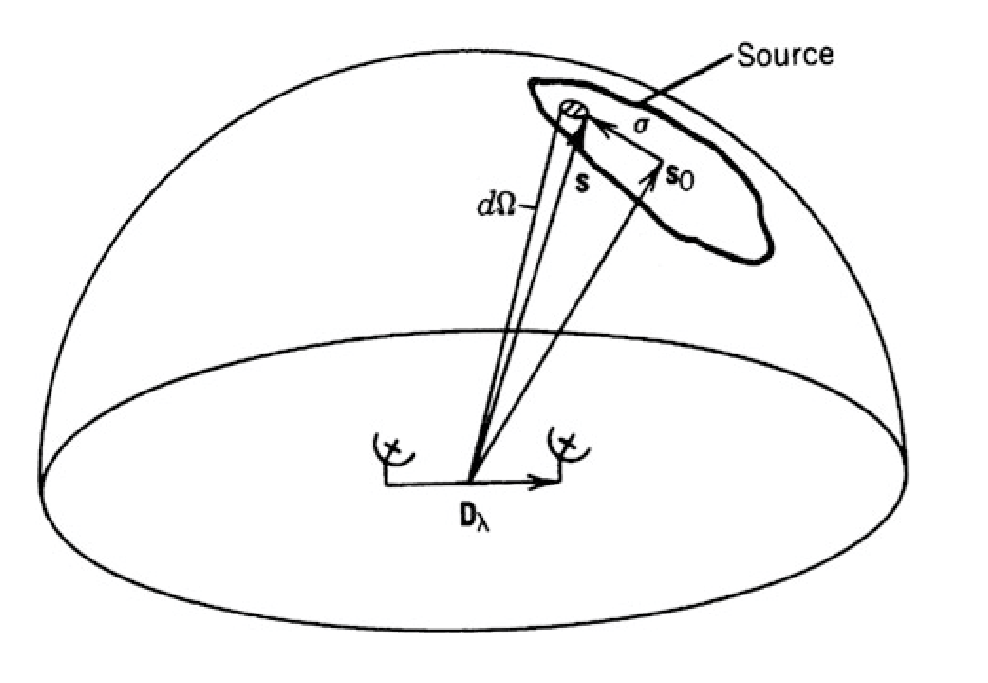
\includegraphics[width=\linewidth]{phasetrack.png}
\label{phasetrack}
\end{figure}
Suppose that antennas track a source under observation,
From the Fig. \ref{phasetrack} , we indicate the phase reference position(\textbf{Phase tracking center}) by unit vector $s_0$.\\
Now, for one polarization, an element of source of solid angle $d\Omega$ at position $s=s_0+\sigma$ has power given by
\begin{equation}
P=\frac{1}{2}A(\sigma)\Delta\nu d\Omega
\end{equation}
Here.
\begin{itemize}
\item $A(\sigma)$ is effective collecting area of each Antenna.
\item $I(\sigma)$ is intensity distribution as observed from the distance. It has  $W \; \; m^{-2}\;\; Hz^{-1} \; \; sr^{-1}$
\item $\Delta \nu$ is the bandwidth of the receiving systems
\end{itemize}
Assumptions made here,
\begin{itemize}
\item The author has made assumptions in eq. (2.1) and (2.2 \textbf{Look into it.})
\item The source is assumed to be at far field.
\end{itemize}
Now the correlator output is $\propto \text{ received power } \times \text{ fringe term } \cos(2 \pi \nu \tau_g)$.\\
The baseline measurements us specified by $\mbf{D_\lambda}$ is measured in wavelenghs and $\nu \tau_g=\mbf{D_\lambda.s}=\mbf{D_\lambda.(s_0+\sigma)}$.\\
Finally, we can write correlator output as
\begin{eqnarray}
r(D_\lambda.s_0) = \Delta \nu \int_{4 \pi} A(\mbf{\sigma})I(\mbf{\sigma})\cos[2 \pi \mbf{D_\lambda.(s_0+\sigma)}]d\Omega\\
=  \Delta \nu \cos[2 \pi \mbf{D_\lambda.(s_0)}]\int_{4 \pi} A(\mbf{\sigma})I(\mbf{\sigma})\cos[2 \pi \mbf{D_\lambda.(\sigma)}]d\Omega \notag\\ 
-  \Delta \nu \sin[2 \pi \mbf{D_\lambda.(s_0)}]\int_{4 \pi} A(\mbf{\sigma})I(\mbf{\sigma})\sin[2 \pi \mbf{D_\lambda.(\sigma)}]d\Omega \label{corout}
\end{eqnarray}
\begin{\cbox}
\textbf{Note:} the integration of the response to the element $d \Omega$ over the source in \eqref{corout}  requires the assumption that the source is spatially incoherent, that is, that the radiated waveforms from different elements $d\Omega$ are uncorrelated. \textbf{This assumption is justified for essentially all cosmic radio sources.} 

\end{\cbox}
Now, let us assume, that $A_0$  be the antenna collecting area in direction $s_0$ in which the beam is pointed.\\
What we no is now introduce $A_N(\mbf{\sigma})=A(\mbf{\sigma})/A_0$ and consider the modified intensity distribution $A_N(\mbf{\sigma})I(\mbf{\sigma})$. We define complex visibility as 
\begin{equation}
\mbf{V}=|\mbf{V}|
\end{equation}


\section{Calibration}
The basic need of calibration is to correct the measured visibility $V^\prime(u,v)$ to approximately as closely as possible to the true visibility $V(u,v)$.\\

The initial calibrated visibilities are corrupted from their true values for numerous reasons, arising from ionospheric or atmospheric effects and from instrumental variations. Common atmospheric effects, for example,
\begin{itemize}
\item include signal attenuation from clouds passing above one antenna but not another
\item radio 'seeing' in which tropospheric water vapour causes phase shifts in the data recorded by one antenna but not another.  
\item Similarly, one antenna might have a defective electronics module that causes large phase drifts or delay jumps that affect data on all baselines to this antenna, but not on other baselines. 
\end{itemize}

 The timescales for these effects can be from seconds to hours, depending on the nature of the effect involved. \\
 It is to be understood that the calibration is not to affect the data from the target source but to correct for disturbances during the observation, primarily due to system's mechanical or electronic defects , powerful radio sources other our target and the  weather conditions. Also to correct for delays introduced as a result of geometric effects as to location of source.
 
\tbf{How do we Calibrate the raw data?}\\
To calibrate the data we must find multiplicative factors for the amplitudes and additive factors for the phases, which, when applied to the raw visibilities, will correct them to the true visibilities.  \\

\tbf{How do we find the above corrective term?}\\
 We can find these correction factors by observing a source whose visibilities have a known form. \\
 If the amplitude or phase of the measured visibilities differs from the expected value, then the correction factor is the number that, when combined appropriately with the visibility, gives the expected value.  These so-called complex gains are complex numbers (i.e. with amplitudes and phases) that multiply the measured visibilities to give the corrected visibilities. This will correct for the systematics in the system during observation.\\
 
 \tbf{Therefore to correct the observational parameters during observation, we need to know the expected value of the visibility.}\\
 \begin{itemize}
\item i.e. The ideal source to use for this calibration is a point source located at the phase center of the field: all baselines should then measure the same amplitude (equal to the flux density of the source) and zero phase. 
\item   In addition to being point-like, a calibrator should be strong (so that only a short observation is needed to detect it) and it should be near to the astronomical source on the sky (so that the atmospheric path followed by the electromagnetic waves is the same for both the calibrator and the source)
 \end{itemize}
 
Therefore summarizing, \tbf{we need a point source for a calibrator which is point source, a strong one and  stable one and also near to the target of out observation i.e. it should not have variations in time and frequency.}\\

\tbf{Do we get such a source that satisfies all the properties and also near to our target source?}\\
 Unfortunately, most point sources are variable, and the few that are stable are unlikely to be nearby to the program source on the sky.  \\
 Therefore, for interferometric observations, we use
\begin{itemize}
\item \tbf{A primary or flux calibrator}
\begin{itemize}
\item It is relatively stable in flux density (on a time scale of years) but possibly far away from the sky. Most commonly are Quasars. Planets can also be used for initial flux calibrator ,particularly at millimeter wavelengths.
\end{itemize}
\item \tbf{a secondary or phase calibrator}
\begin{itemize}
\item Phase calibrator is variable on much shorter timescales but is very near to our target source
\end{itemize}
\end{itemize}

\tbf{What does a common observation looks like?}\\
 \begin{itemize}
\item first observe the flux calibrator and use this to calibrate \tbf{the amplitudes of the phase calibrator}. 
\item The phase calibrator, then, serves to calibrate the visibility amplitudes and phases for the remainder of the observation. (It helps to take care of ionospheric and turbulent effects in the atmosphere.  The idea is that just before and just after observing the program source, we can determine the gains that will correct the data for atmospheric and instrumental effects. ).\tbf{\tit{At times between the calibration scans, when we are observing the program source, we apply interpolated values of the gains to calibrate the visibility data. }}
\end{itemize}

 We generally intersperse short scans of the phase calibrator throughout the observing period. \\
 
 \tbf{How often one observes, phase calibrator ?}\\
 The answer to this depends on how drastically the instrument or the atmospheric conditions change. \tbf{The assumption on calibration is based on the assumption that any changes can be corrected till they are of first order or linear}. If  the instrument or the atmosphere changes too drastically between calibrator scans, the assumption that we can track these changes by linear interpolation will no longer be valid. \\
 
 Therefore,the observation of Phase calibrator depends on: 
 \begin{itemize}
 \item  \tbf{Observing Frequency}:  (more frequent scans at higher frequencies)
 \item \tbf{The Baseline length}:  (more frequent scans when observing with longer baselines) 
 \item \tbf{the weather}: (more frequent scans in poor weather conditions)
\end{itemize}  

So Far so good, but
\tbf{Is it okay if we observe the phase calibrator too many times during observation?}\\
 the time spent observing calibrators is time not available to observe the program source.  Thus, we don't want to observe the calibrators for more time than is necessary.\\
 
\tbf{Therefore how can we define a minimum for the number of times spent in observing a phase calibrator?} 
\begin{itemize}
\item    The basic requirement is that each baseline should detect the calibration source.
\item A common guideline is that the calibrator should be observed for enough time that its accumulated visibilities on a single baseline will give a \tbf{SNR of at least 5}
\end{itemize}   

It is to be noted that:\\
\tbf{each calibrator scan should have SNR  > 5.  For the program source we can combine many scans to improve the SNR, but for calibration each scan alone must meet the SNR requirement. }\\

\tbf{Bandpass Calibration}\\

When observing in spectral-line mode \tbf{(with many channels at slightly different frequencies)} a bandpass calibration is usually needed.  This is done by observing a bright continuum source of known spectral shape and then calculating frequency-dependent complex gain factors that will make the observed spectrum agree with the true spectrum.\\

Note:  To avoid adding noise to the target spectrum, the bandpass spectrum should have a higher SNR. Now doubling the SNR of an observation requires a factor of 4 increase in time, so a bandpass calibrator much brighter than the target source is desirable.   Continuum bandwidths are not routinely greater than 1 GHz.  To avoid \tbf{bandwidth smearing} and to aid in RFI excision, it is advantageous to channelize these wide bandwidths.  Thus, even continuum observations are made in a spectral-line observing mode and hence require a bandpass calibration. 



Now for a synthesis array, the fundamental equation is:
\begin{equation}\label{eq:compvis}
V(u,v)=\int A_\nu(l,m)I_\nu(l,m)\exp[-2 \pi (u l+vm)]dl dm 
\end{equation}
here
\begin{itemize}
\item $\nu$ is the frequency of radiation
\item (l,m) are direction cosines with respect to phase center.
\item (u,v) are the projected baseline coordinates in wavelengths i.e. $u=B_{l,\lambda}\;,\;v=B_{m,\lambda}$
\item $V(u,v)$ is the true visibility evaluated at $(u,v)$.
\item $A_\nu(l,m)$ is the normalized beam pattern(pattern of a single antenna)
\item $I_\nu(l,m)$ is the brightness distribution of the source.
\end{itemize}

And the exponent comes from $B_\lambda \dot s = ul+vm+wn=wl+vm+\tau_g v$ and when we say "with respect to the phase center", we mean that the group delay is compensated so that $\tau_g v=0$\\

We can re-write his to emphasize the discrete sampling with antenna pair $i,j$ at times t by:
\begin{equation}
V_{i,j}(u,v)=\int A_\nu(l,m)I_\nu(l,m)\exp[-2 \pi (u_{i,j} l+v_{i,j} m)]dl dm 
\end{equation}
and $ul+vm$ is the geometric phase difference $\Delta \phi$ produced by the differential path length  between antenna i and antenna j  from the part of source at location (l,m) relative to the phase center.\\

Before that, we have to check if there is a geometric phase difference at the phase center i.e. at l=m=0 and find the w term.\\
Recall that,
of the hour angle and declination of the source co-ordinates are $h_0,\delta_0$ and the baseline lengths are $B_x,B_y ,B_z$ . Then the geometric phase difference at the phase center (the w term at l=m=0)\fn{I have to look what exactlyis this argument} is 
\begin{eqnarray*}\label{eq:geodiff}
\phi_g=2 \pi \tau_g \nu \\
\implies \phi_g=\cc{2\pi/\lambda}\rr{B_x \cos \delta_0 \cos h_0 - B_y \cos \delta_0 \sin h_0 + B_z \sin \delta_0} 
\end{eqnarray*}
The above equation is the basis for all iterferometric analysis of antenna position coordinates and the basis for determination of astronomical positions.\\
Now, let us see what can cause the geometric phase difference even at phase center, \tbf{This is done by taking a differential of \eqref{eq:geodiff} to just first order}:
\begin{eqnarray*}
d\phi_g=2 \pi \nu d \tau_g\\
\implies d\phi_g= (2\pi /\lambda)[dB_x  \cos \delta_0 \cos h_0 - dB_y  \cos \delta_0 \sin h_0 +dB_z \sin \delta_0 \\
\;\;\;\;\;\; +d\alpha_0 \cos \delta_0 \cc{B_x \sin h_0 + B_y \cos h_0} \\
\;\;\;\;\;\; +d\delta_0 \cc{-B_x \cos h_0 \sin \delta_0 + B_y \sin h_0 sin \delta_0 +B_z \cos \delta_0}]
\end{eqnarray*}
where, $h_0=LST-\alpha_0$ or $ d h_0=-d \alpha_0$. The above shows how baseline errors $(dB_x,dB_y,dB_z)$ and source position errors $(d\alpha_0 ,d\delta_0)$ will affect the error in group delay $d \tau_g$ or yield an error in phase $d \phi_g$.\\
\tbf{Note: a clock error is equivalent to a source position error $d \alpha_0$}
\subsection{Interferometric Response}

An interferometric array generates the observed visibilties $V^\prime_{ij}(t)$. A properly designed synthesis array will preserve a linear relationship between the measured visibilities $ V^\prime(u,v) $ and the actual visibilities $ V(u,v) $ .Furthermore, the individual measurements are well isolated: i.e. the reponse associated with one pair of antennas doe snot depend on other pair of antenna.\\


The basic antenna pair response is expressed as:
\begin{equation}
V^\prime_{ij}(t)=G_{ij}(t)V_{ij}(t)+\epsilon_{ij}(t)+\eta_{ij}(t)
\end{equation}
where, t is the time of observation
So we have two unrequited components:
\begin{itemize}
\item Baseline based complex -Offset($\epsilon_{ij}$)
\item Stochastic complex noise term($\eta_{ij}$)
\end{itemize}
$G_{ij}$ is the baseline complex gain for the \tit{ij-th} baseline. The equations are complex and represents the two output of each correlator the \tit{sine correlator and the cosine correlator}  through the real and imaginary part of complex quantity\\
Now, during the observation, the visibilities are averaged over a time interval during which they, or the complex gains, are not expected to change enough so as to lower the coherence. \tbf{Since the field of view of the antenna primary element limits the region from which signals are received, the maximum rate of change of phase will come come from points at the edge of this region\fn{why so?}}\\
\begin{\cbox}
This limits the maximum the maximum integration time in seconds, which is then given by $\Delta t_{int}\sim 2D_{(m
)}/B_{(km)}$ where $D_{m}$ is the diameter of antenna in meters and $B_{(km)}$ is the length of the baselines in kilometers. Longer time intervals are permissible if the angular extent of the source is less than the primary beam size. The permissible integration-time scales with the ratio of the primary beam size to the source angular size.
\end{\cbox}
\subsection{Calibration Methods}
The choice of calibration, depends on both the design of the array and the severity of problem. Calibration can be classified into 3 basic categories:
\begin{itemize}
\item Direct Calibration:
\item Calibrator sources in the sky: 
\tbf{Does interferometer have a  actual phase reference?}\\
An interferometer measures phase reference so there is no absolute phase reference.\\

\tbf{For any observation we wish to reference visibility phases to the phase tracking center(which in general is same as the center of the primary antenna beam}.\\

Therefore to determine the antenna phase offsets, observation of a sky calibrator is required.\\

Now, if the array is not again phase or gain stable , \tbf{periodic observations are used to monitor these changes. In addition time variable phase changes occur in the data, which again requires observations of calibrator source to remove this effect.}

\item Self Calibration: In some cases the sources being observed can be used as a test signal to calibrate the instrument. This calibration requires \tbf{strong signals and particular array properties}
\end{itemize}


\subsection{Calibration of phase and amplitude}
\tbf{Most data corruption occurs before the signal pairs are correlated} , so that the baseline complex gains $G_{ij}$ can be approximated by the product of the two associated antena based complex gains $g_i (t)$ and $g_j(t)$
In terms of individual antennas the complex gains can be expressed as gains of individual antennas:
\begin{equation}
G_{ij}(t)=g_i(t)g_j^star(t)=a_i(t)a_j(t)\exp{\rr{i\cc{\phi_i(t)-\phi_j(t)}}}
\end{equation}
Here $a(i)$ is the \textbf{antenna based amplitude correction} and $\phi_i$ is the antenna based phase correction. Observation of calibrator sources determine $G_{ij}$ for each of the $N(N-1)/2$ baselines, when N is the number of antennas.


\subsection{Multi-frequency and dual polarization capability}
\subsection{Initial Calibration}
\tbf{Before antenna can be put to observation, instrument parameters must be determined}. It includes the antenna pointing, delays and positions. Another related parameter is the accurate position of the calibrator to be used for monitoring system gain. This section describes these calibrations. \tbf{In almost all cases the parameters describing these effects must be determined and applied before useful observing can begin.}
\subsubsection{Antenna pointing and gain}
\tbf{The fundamental formulation of \eqref{eq:compvis} assumes that the primary beam distribution $A_\nu(l,m)$  is independent of time and identical for each antenna.}\

\tit{Small deviations may occur, some of which can be corrected during observation}.\\

It is requisite that the antennas are able to track the diurnal motion of the source, i.e. the change in orientation of an antenna must be fast enough to track the target source. \\

\tbf{If you have antennas of two different primary beam shapes given by $A_\nu(l,m)$ then only those sources for which the angular size of the object as seen by antenna is smaller compared with the angular size of the primary beam, unless sophisticated imaging software is used.}\\

\tbf{Q. How accurate should the center of primary beam track the intended sky position?}\\
The tracking of the intended sky position must be better than $1/10^{th}$ of the Full Width to Half Power of the primary beam, else the sensitivity of the observations would be reduced. The 0.1 FWHP tolerance should be even smaller if the path of the primary beam contains emission, either from one large diameter source or from a high density of background source.\\

\tbf{What is antenna pointing error?}\\
Antenna pointing error is the difference between actual antenna pointing (location of the center of the primary beam ) and the desired position.\\

This error may have directional dependence:
\begin{itemize}
\item misalignment of the polar or elevation axis
\item gravitational deformation of the structure
\item non perpendicularity of the two axis
\item atmospheric refraction and other effects
\item differential heating of the structure may induce time dependent error
\item wind loading may also cause variation with time scales of seconds
\end{itemize}

\textbf{Q.How do we sort out this error?}\\
This error can be sorted out :
\begin{itemize}
\item by optical alignment with polaris and other bright stars which can determine the pointing accuracy within 10 arc minutes
\item higher accuracy requires observations in many parts of sky with known radio sources
\item these parameters are then fitted to a physically meaningful mathematical model describing antenna defects
\end{itemize}

\tbf{What are the standard observations used to determine the pointing position from a calibration source?}\\
\begin{itemize}
\item Total power observations.\\

These can be done by a single telescope observing bright extended sources.
\item interferometric observations

They have better stability
\end{itemize}

Finally the gain of antenna is also related to position w.r.t zenith as observations are made near the horizon, the gain decreases because of the deformation of the antenna structure and surface.\\

If the intensity of a calibrator source is known then one can measure , as a function of zenith angle , the ration of visibility amplitude to intensity.\\





\begin{itemize}
\item \textbf{Antenna Pointing and Gain}: our equation for inverting the visibilities assumes that the normalized antenna primary beam distribution $A(l,m)$ is independent of time and identical for each antenna. \\
Ideally the antenna tracking center must follow the same intended position for all antennas (In general it can referred to as the phase tracking center.) . The error in this tracking can cause reduced sensitivity and distortions in extended objects.\\

For point sources: the tracking accuracy should be $0.1\theta_{FWHM}$ where, $\theta_{FWHM}$= angular size of FWHM of the primary beam.\\
Extended objects like Sun, covers a large part of the primary beam , the pointing accuracy should be better $\theta_{FWHM}$ .\\

This antenna pointing error is the difference between the actual pointing position and the desired one. The pointing error is a directional dependence due to
\begin{itemize}
\item misalignment of antenna rotation axes
\item gravitational deformation
\item non perpendicular axes.
\item atmospheric refraction
\item wind loading
\item differential heating of the structure.
\end{itemize}

\item \textbf{Delay Calibration}:an error in delay of only a few nanoseconds will cause the different parts of the observing band to partially interfere (different frequencies in the band arrive with different phase), leading to a drop in the amplitude.  Obviously, we need to have the delays optimized.

\item \textbf{Time and Place:} The time and location of the antennas must be known to relatively high accuracy. -- needed for determining the geometric delay.  A clock error of 1 s, or a baseline error of a few cm, will cause a serious phase shift of the source over, say, 10 minutes. 
\end{itemize}

\subsubsection{Delay Calibration}
The antenna based visibility equation \eqref{eq:compvis} is a monochromatic synthesis equation. For Modern arrays, the instruments are designed to work over large bandwidths, therefore \tbf{the frequency response over the desired bandwidth must be coherent}. Large bandwidths, of course , are required to obtain sufficiently high signal to noise from the weak celestial sources.\\
For a finite bandwidth, the integrated visibility function is 
\begin{equation}
V_{ij}=\int^\infty _{0}\cc{\int^\infty _{-\infty} \int^\infty _{-\infty}A_\nu(l,m)I_\nu(l,m)e^{-2\pi i \nu \Delta\tau_g}dl dm}e^{2\pi i \nu \Delta \tau_r}G_{ij}(\nu)d\nu
\end{equation}

Here $G_{ij}$ is the complex gain as a function of frequency and $\Delta \tau_g$ is the differential geometric delay for the i-j baseline (Delay relative to the delay tracking center). $\Delta \tau_r$ is the residual instrument delay for the i-j baseline(the error in inserted delay for the delay tracking center)\\

If $\Delta \nu$ is used to denote the spanned bandwidth of the observations, then the phase difference $\Delta phi$ between the ends of the band, the result from a net residual delay $\Delta \tau_g -\Delta \tau_r$ is given by,
\begin{equation}
\Delta \phi = 2 \pi \Delta \nu (\Delta tau_g -\Delta \tau_r)
\end{equation}.\\


\tbf{It is important to understand the loss of coherence is only parametrised by phase and not the gain amplitude. } Therefore if $\Delta phi$ is greater than about one radian than a significant loss of coherence across the band will occur. \tbf{Thus the delay must be less than about $(160/\Delta nu)$ nanoseconds, assuming $\Delta \nu$ is expressed in MHz.}\\

\tbf{Q. What is the origin to delay error?}\\

Ans. \begin{itemize}
\item Geometric delay(with respect to delay tacking center): Can be compensated through insertion of delay in the system 
\item the errors in inserted delay : This is either due to mis-calculation or mis-calibration of the required delay or due to inevitable quantization of inserted delay. Even though geometric delay is well calculated but the above defined additional error may arise as a result \tit{signal propagation times through the different electronic paths. This may also vary for a single antenna for different frequencies and polarization}
\end{itemize}

\tbf{Q. How do we correct for this error?}
Ans. This can be corrected by observing a strong, isolated source of emission and vary the delay in small steps \tbf{until the maximum in the coherence can be found}.
\subsection{The antenna primary beam}
The visibility function measures the spatial coherence function of a fictitious source given by $A(l,m)I(l,m)$. By spatial coherence , we mean that coherence depends on spatial co-ordinates (l,m) and coherence is higher for higher visibility amplitude. Therefore , it becomes crucial to remove the effect of primary beam sensitivity carried by the term $A(l,m)$ must be removed from the image. \tbf{Read this later. Deals with polarization}
\subsection{Bandwidth Smearing}
\tbf{What is bandwidth smearing?}\\
Chromatic Aberration or Bandwidth smearing is observed when observations are made over large instantaneous bandwidths, then distortions occur in parts of the image far removed from the phase center. \\

\tbf{When should we be concerned of this chromatic observation?}\\
As a rule of thumb, One should be concerned or chromatic aberration becomes significant when the offset, measured in units of synthesized beamwidths, and multiplied with fractional bandwidth, is of order unity. It produces a radial smearing whose shape is the effective bandpass convolved with the source structure.  


\tbf{How do we avoid bandwidth smearing?}\\
Bandwidth smearing can be avoided by separating th observations into a set of narrowed bandwidth channels by using filters or by cross correlation techniques in which many delay centers are used.

\section{Point Source Function}
The point spread function (PSF) describes the response of an imaging system to a point source or point object. \\

For radio telescopes and diffraction-limited space telescopes, the dominant terms in the PSF may be inferred from the configuration of the aperture in the Fourier domain.\\

Now the visibility function is sampled at a finite number of spatial frequencies:\\

Therefore:
\begin{eqnarray*}
V^{obs}(u,v)=S(u,v)\cdot V(u,v)\\
\implies F^{-1}\rr{V^{obs}(u,v)}=F^{-1}\rr{S(u,v)\cdot V(u,v)}\\
\implies I^{obs}(l,m)=F^{-1}\rr{S(u,v)}\star F^{-1}\rr{ V(u,v)}\\
\implies I^{obs}(l,m)=I^{psf}(l,m)\star I^{sky}(l,m)\\
\end{eqnarray*}
Therefore the observed image is a convolution between the point spread function and the true sky brightness distribution.\\

Therefore the PSF is the inverse Fourier transform of the UV coverage. The PSF is :
\begin{itemize}
\item The impulse response of the instrument (i.e. image of a point source) \\
\item The intensity of the diffraction pattern through an array of slits (dishes)\\
\item a measure of the imaging properties of the instrument
\end{itemize}
The angular separation hence would be related to max uv spacing, therefore point sources might resolve out for very long baselines \\
\section{Deconvolution of dirty image}
The inverse F.T. of observed Visibility would give us dirty image and the process of deconvolution separates the PSF from the sky brightness distribution.
\subsection{Imaging in practise}
\begin{enumerate}
\item  \tbf{Choosing image coordinates}
\tbf{Choosing image 'cell size':}Nyquist sample the main lobe of the PSF.\\

PSF beam width is given by:
\begin{equation}
\frac{\lambda}{b_{max}}=\frac{1}{u_{max}}\;\;radians(\times \frac{180}{\pi}\;\; to \;\; convert \;\; to \;\; degrees)
\end{equation}
\tbf{Choosing number of pixels:} That would determine the field of view being sampled (This can be as much desired or what is practical for the science case.)\\

The field of view controls the uv grid cell size($\delta u, \delta v$):\\
\begin{equation}
\frac{1}{fov_{rad}}=\delta u
\end{equation}
\item \tbf{The uv plane is sampled irregularly (along uv tracks):}\\
But, we use the Fast Fourier transform to form the image.
\item \tbf{Measured visibilities contain noise; and also some uv ranges may be sampled more than others}\\
Therefore, we need to choose how to weight the visibilities during imaging.

\end{enumerate}
\section{CASA Theory}

\subsection{Flagging}
Refer to $https://casa.nrao.edu/casadocs/casa-5.4.0/global-task-list/task \_flagdata/about$\\

The command we use here is \tit{flagdata}.\\
It can basically flag data from \tbf{measurement sets or calibration table}. It can be used tin overall two ways:
\begin{itemize}
\item Directly by setting parameters for flagging
\item BY input a script
\end{itemize}

The available modes are 
\begin{itemize}
\item \tit{manual}: will flag based on the parameters set by the user
\item \tit{clip}(\tbf{auto-flagging algorithm}): clip parameters based on a specific selection of parameters
\item \tit{shadow}
\item \tit{quack}: will remove specific time ranges at the beginning or end. we basically specify the time interval and where to flag.
\item \tit{elevation}: will remove the data above or below a certain elevation
\item \tit{tfcrop}(\tbf{auto-flagging algorithm}): this algorithm finds and flags outliers based on polynomial fit in the time-frequency plane
\item \tit{rflag}(\tbf{auto-flagging algorithm}): This algorithm finds and flags outliers based on sliding window RMS filters
\item \tit{extend}: mostly used after automatic flagging algorithm where the user can grow or extend the flags further beyond those detected by the automatic algorithms
\item \tit{unflag}: unflags a particular data
\item \tit{summary}: this helps to report th amount of data flagged
\end{itemize}
Further, each of the above mode, requires certain other parameters which are specific to that mode. One can check those in the \tbf{expandable parameters set} in the described  website and if not specified, default values for these \tbf{expandable parameters} would be taken in.
\begin{\cbox}
The current flags can be automatically backed up before applying new flags if the parameter \tit{flagbackup} is set. Previous flag versions can be recovered using the \tit{flagmanager} task.
\end{\cbox}
\tbf{Q. What are the essentials to be input?}\\
\begin{itemize}
\item \tit{vis:} user needs to enter the name of the visibility file or calibration table which is needed to the flag
\item \tit{mode:} user has to set the mode of operation depending on how they want to handle data.
\end{itemize}
I will discuss some important components only for automatic flagging algorithms , because that will be definitely used.\\

\tbf{Expandable parameters (common to all auto-flagging algos):}\\
\begin{itemize}
\item \tit{ntime:} Set the time range (in seconds or minutes) over which to buffer data before running the algorithm. Therefore , depending on the specified time range, the data sets would be iterated in time chunks. \tit{Does a smaller range or chunk gives a more aggressive flagging?}
\item \tit{combinescans:} When set to True, it will remove SCAN from the sorting columns, therefore it will only accumulate across scans if \tit{ntime} is not set to 'scan'. \tit{I don't understand the meaning here}
\end{itemize}
Let us  look into \tit{tfcrop mode}:\\
The following things happen:\\
For each field, spw, timerange (specified by ntime), and baseline:
\begin{enumerate}
\item Average visibility amplitudes along time dimension to form an average spectrum
\item Calculate a robust piece-wise polynomial fit for the band-shape at the base of RFI spikes. Calculate 'stddev' of (data - fit).
\item Flag points deviating from the fit by more than N-stddev
\item Repeat (1-3) along the other dimension.
\end{enumerate}

This algorithm is designed to operate on un-calibrated data (step (2)), as well as calibrated data. It is recommended to extend the flags after running this algorithm.\\

Now, let us look into some expendable parameters that goes in this algorithm:
\begin{itemize}
\item \tit{timecutoff}: It is the Flag threshold in time. Flag all data-points further than N-stddev from the fit. This threshold catches time-varying RFI spikes (narrow and broad-band), but will not catch RFI that is persistent in time. Flagging is done in up to 5 iterations. The stddev calculation is adaptive and converges to a value that reflects only the data and no RFI. At each iteration, the same relative threshold is applied to detect flags. (Step (3) of the algorithm).
\item \tit{freqcutoff}: Flag threshold in frequency. Flag all data-points further than N-stddev from the fit. Same as timecutoff, but along the frequency-dimension. This threshold catches narrow-band RFI that may or may not be persistent in time.
\item \tit{timefit} : Fitting function for the time direction. Default: 'line'. Options: 'line', 'poly'.\\

A 'line' fit is a robust straight-line fit across the entire timerange (defined by ntime). A 'poly' fit is a robust piece-wise polynomial fit across the timerange. 
\item \tit{freqfit} : Fitting function for the frequency direction. Same as for the timefit parameter. Default: 'poly'. Options: 'line', 'poly'. Choose 'line' only if you are operating on bandpass-corrected data, or residuals, and expect that the bandshape is linear. The 'poly' option works better on uncalibrated bandpasses with narrow-band RFI spikes.
\item \tit{maxnpieces}:Maxinum number of pieces to allow in the piecewise-polynomial fits. Default: 7. Options: 1 - 9. This parameter is used only if timefit or freqfit are chosen as 'poly'. If there is significant broad-band RFI, reduce this number. Using too many pieces could result in the RFI being fitted in the clean bandpass. In later stages of the fit, a third-order polynomial is fit per piece, so for best results, please ensure that nchan/maxnpieces is at-least 10.
\item \tit{flagdimension}: Choose the directions along which to perform flagging. Default: 'freqtime'; first flag along frequency, and then along time. Options: 'time', 'freq', 'timefreq', 'freqtime'. For most cases, 'freqtime' or 'timefreq' are appropriate, and differences between these choices are apparant only if RFI in one dimension is significantly stronger than the other. The goal is to flag the dominant RFI first. 
\item \tit{usewindowstats}:Use sliding-window statistics to find additional flags. Default: 'none'. Options: 'none', 'sum', 'std', 'both'
\item \tit{halfwin}:Half width of sliding window to use with usewindowstats. Default: 1 (a 3-point window size). Options: 1,2,3
\end{itemize}
\subsection{Calibration}
First we set flux densities are set for the standard flux calibrator in the data.
\subsubsection{Absolute flux calibration}
First we need to set the model column with the visibilities of a calibrator using \tit{setjy}. This task places the model visibility amp and phase associated with a specified clean components image into the model column of the data set. \tit{setjy} need only be run on the calibrator sources with a known flux density and/or model.
\subsection{Delay and Bandpass Calibration}
First we will do delay calibration. In calibration, a reference antenna is required. First, run \tit{gaincal} to solve for an initial set of antenna-based phases over a narrow range of channels. To find channels for each spectral window that are relatively RFI-free over the course of the observing session, look at the data with plotms. Use only a narrow channel range.\\

The gaincal, bandpass, polcal, and blcal tasks actually solve for the unknown calibration parameters from the visibility data obtained on calibrator sources, placing the results in a calibration table. They take as input an MS, and a number of parameters that specify any prior calibration tables to pre-apply before computing the solution, as well as parameters controlling the exact properties of the solving process.\\

In all of the above tasks The gaintable parameter takes a string or list of strings giving the names of one or more calibration tables to arrange for application.

So we need:
\begin{itemize}
\item frequency based calibration for all channel : \tbf{done through \tit{bandpass}}
\item time based calibration  for temporal errors: \tbf{done through \tit{gaincal}}
\end{itemize}
\tbf{Q. What is Bandpass calibration?}\\

Ans. Calibration of frequency based response of the system , problems in which can arise due to receivers intrinsic response , delay offsets, cable attenuation and antenna chromatism.\\

\tbf{ For this A strong quasar is observed at the beginning of each project} for which
\begin{itemize}
\item Phase vs frequency should be zero (point source) 
\item Amplitude vs frequency should be constant (continuum source)
\end{itemize}

The above conditions must be met for all baselines i.e. same visibility must be obtained for a strong point source. \\

\tbf{How do we do it?}\\
\begin{itemize}
\item Time average over one scan (to improve SNR) 
\item  Time average over several scans (then need a phase calibration first of these scans) 
\item Solve for antenna based gains
\item Fit amplitude and phase vs frequency (polynomials)
\item Assume bandpass is constant with time • Must be recalibrated if receiver is retuned
\end{itemize}
\tbf{What is bandpass function}\\
Determines the amplitude and phase as a function of frequency for each spectral window containing more than one channel. Strong sources (or many observations of moderately strong sources) are needed to obtain accurate bandpass functions. The two solution choices are: Individual antenna/based channel solutions 'B'; and a polynomial fit over the channels 'BPOLY'. The 'B' solutions can determined at any specified time interval, and is recommended in most applications. 

\tbf{Q. What is gaincal?}\\

\tbf{Ans. Objective is to Determine temporal gains from calibrator observations} i.e. calibrates time based response for the system\\
The complex gains for each antenna/spwid are determined from the data column (raw data), divided by the model column, for the specified fields. The gains can be obtained for a specified solution interval for each spectral window, or by a spline fit to all spectral windows simultaneously.\\

Gaincal corrects short time  based phase variation due to atmosphere  and also long term variation like antenna position error or antenna electronics. This requires us to observe a quasar for every 20 minutes  basically a phase calibrator .\\

Gaincal also corrects for time based amplitude problems as a result of antenna efficiency issues over long runs for which it Needs amplitude referencing to a point source (quasar) to calibrate the time variation of the antenna efficiency (cf phase calib).\\

\tbf{Q. What is fluxscale?}\\

Ans. The whole need is to get the flux density for phase calibrator correct i.e. Need to measure known fluxes against monitored Planets, strong, strong quasars. So that once we have determined the gain amplitude we should be able to find results for known sources.
\begin{itemize}
\item After running gaincal on standard flux density calibrators (with or without an image model), and other calibrators with unknown flux densities (assumed 1 Jy) \tit{meaning phase calibrator, because we don't load model flux for phase calibrators}, \tbf{fluxscale applies the constraint that net system gain was, in fact, independent of field, on average, and that field-dependent gains in the input caltable are solely a result of the unknown flux densities for the calibrators.}
\item Using time-averaged gain amplitudes, the ratio between each ordinary calibrator and the flux density calibrator(s) is formed for each antenna and polarization (that they have in common).
\item The average of this ratio over antennas and polarizations yields a correction factor that is applied to the ordinary calibrator's gains. (See also more detailed discussion in Example section below.)
\item For incremental=False(default), the median of this ratio over antennas and polarizations yields a correction factor that is applied to the ordinary calibrators’ gains. For incremental=True, only the correction factors are written out to the output fluxtable[\tit{Name of output, flux-scaled calibration table}].  
 
\end{itemize}
\subsection{CASA Imaging}
\subsubsection{Self Calibration}
\begin{enumerate}
\item Till now we have done a priori calibration from external calibrators which are interpolated from
different time and sky direction from source. Now this may leave error.
\item \tbf{What does self calibration do?}\\

self calibration corrects for antenna based phase and amplitude errors together with imaging to create an improved source model . \tit{No more testing the source against the calibrator is required.}

\item \tbf{Why should this work?}\\
\begin{itemize}
\item at each time,we measure N complex gains and get a total of N(N-1)/2 visibilities
\item source structure can be represented by small number of parameters
\item Hence this becomes an overconstrained problem if N is large and source is simple
\end{itemize}
\item \tbf{What do we exactly do during the self cal?}\\
\begin{itemize}
\item assume source model $\rightarrow$ solve for time dependent gains $\rightarrow$ form new source model from corrected data using clean $\rightarrow$ solve for new gains
\item requires sufficient signal-to-noise at each solution interval \tbf{What does this line mean?}
\end{itemize}
\item \tbf{What is the downside of the process?}
\begin{itemize}
\item loses absolute phase from calibrators and therefore position information
\item dangerous with small N arrays, complex sources, low signal-to-noise
\end{itemize}
\end{enumerate}
\newpage
\section{Imaging}
\subsection{Fourier Transform Imaging}
A fundamental result of the first chapters is that there exists a fourier transform relationship between the sky brightness \tit{I}, the antenna beam pattern \tit{A} and the visibility \tit{V} observed with an interferometer.
\begin{equation}\label{eq:modI}
A(l,m)I(l,m)=\int^\infty _{-\infty} \int^\infty _{-\infty} V(u,v) e^{2 \pi i(ul+vm)}du dv
\end{equation}
This relation holds when
\begin{itemize}
\item $|\frac{\Delta \nu}{c}\cc{\mbf{s-s_0}}|<<1$
\item $|w(l^2+m^2|<<1$
\end{itemize}
Now the above two conditions are met \tit{whenever the radiation to which interferometer originates from a small region in sky.}\\

\tbf{Now, if we assume that we know what $A$ is like over large regions in sky $(l,m)$ then we shall use $I(l,m)$ instead of $A(l,m)I(l,m)$ as modified surface brightness. We can correct for $A(l,m)$ in the last stages of data processing to get the right sky brightness distribution.}\\

\begin{\cbox}
For widefield imaging, if a source covers a region which is larger than the central lobe of the primary beam, is a problem. Because than the source starts convolving with sidelobes, which would depreciate the quality of image and create psf based artifacts.
\end{\cbox}

So to set our checkboxes straight:
\begin{itemize}
\item $V$ is a complex quantity measured in units of flux density ('Jansky',$1Jy=10^{-23}$ ergs $cm^{-2} \;\; s^{-1} \;\; Hz^{-1}$ )
\item $I$ is the real sky distribution and is given by flux density/beam area or sometimes Jy per square arcsecond.
\end{itemize}

So once you obtain visibilities over (u,v) points given by $(u_k,v_k)$ where $k=1, \cdots ,M$, where M represents the array elements, it is just a matter of model fitting or fourier transform, whichever is less computational, to obtain the estimate of modified sky brightness.\\

Here, we discuss just how to approximately calculate right hand side of \eqref{eq:modI}, or the so-called \tbf{"Dirty Image"} given by $I^D$
\begin{equation}\label{eq:DirtyI}
I^D(l,m)=\int^\infty _{-\infty}  \int^\infty _{-\infty} S(u,v) V^\prime (u,v) e^{2 \pi i(ul+vm)}du dv
\end{equation}
where S is the (u,v) sampling function and $V^\prime$ is the observed visibility, here \tbf{the prime is an indicator if noise corrupted measurements}, even if $I^D$ is not primed, it too has noise components.

\subsection{The \tit{Direct Fourier Transform} and FFT}
You heard it correct, it is \tit{Direct Fourier Transform} and not the popular DFT or Discrete Fourier Transform.\\

 So we compute the dirty image either from \tit{Direct Fourier Transform} or FFT.\\
 
 \begin{itemize}
 \item \tit{Direct FT:} The dirty image is given by
 \begin{equation}
 \frac{1}{M}\sum^M _{k=1} V^\prime (u_k,v_k)e^{2 \pi i(u_k l+v_k m)}
 \end{equation}
 If we want to evaluate the Direct FT of an $N \times N$ grid, then the number of real multiplications is $4MN^2$(Assuming the data is hermitian, the number is halved).\\
 
 Normally M is of the same order as $N^2$ so the the number of calculations go as order of $N^4$. The number of sine and cosine evaluation is also of order of $N^4$\\
 
 \item \tit{Via FFT:} Here we need to interpolate the data on a rectangular grid, so that a FFT algorithm can be used. \tbf{The process of interpolation is called gridding}\fn{'gridding' the data may require the data to be sorted in order of decreasing |u| or decreasing |v|.} The number of arithmetic operations required here are of $O(\text{M})$. The number of operation required by FFT is $N^2\log_2 N$. So it has very less computation for Large N. 
 \end{itemize}
 \tbf{But if your N is small, go with Direct FT}
\subsection{The Sampling Function and Weighting The Visibility} 
\begin{\cbox}
The Sampling Function is the Fourier Transform pair of the synthesized beam B. 
\end{\cbox}
\subsection{The Sampling Function}
\tbf{Q. Define the Sampling function.}\\

S is a generalized function or distribution which is defined as 2-dimensional Dirac delta function
\begin{equation}\label{eq:sampling}
S(u,v)=\sum^{M}_{k=1} \delta(u-u_k,v-v_k)
\end{equation}

Now as a result of sampling the visibility we define,\\

\tbf{The Sampled Visibility Function} or 'measurement distribution'\\
\begin{equation}
V^S(u,v)\equiv \sum^{M}_{k=1}\delta(u-u_k,v-v_k)V^\prime (u_k,v_k)
\end{equation} 
which is equivalent of $V^s=SV^\prime$.

\tbf{Q. How do we express the dirty image in terms of noise filled Visibility data?}\\
\begin{eqnarray*}
I^D=F.T.[V^S]=F.T.[SV^\prime]\\
\implies I^D=F.T.[S]\star F.T.[V^\prime]
\end{eqnarray*}

\tbf{Define a Synthesized Beam B}\\

Point source response of the array i.e. when $V^\prime(u,v)\equiv 1$, for a point source , centered at position $(l_0,m_0)$ and $F.T.[V^\prime]\equiv \delta(l-l_0,m-m_0)$ is the synthesized beam 
\begin{equation}
B=F.T.[S] \star \delta=F.T.[S]
\end{equation}
\begin{\cbox}
Therefore, the observed brightness is the true brightness convolved with the beam
\end{\cbox}
\subsubsection{Weighting Functions for control of the beam shape}
\tbf{Q. Define the weighted sampling function.}\\

A weighted sampling function is defined as 
\begin{equation}
W(u,v)=\sum^{M}_{k=1} R_kT_kD_k \delta(u-u_k,v-v_k)
\end{equation} 

\tbf{Q. Now, we would like to define a weighted sampled visibility function and sampled measurement distribution $V^W$}\\

The sampled distribution is given as $V^W=WV^\prime$, or ,
\begin{equation}
V^W(u,v)\equiv \sum^{M}_{k=1}R_k T_k D_k\delta(u-u_k,v-v_k)V^\prime (u_k,v_k)
\end{equation} 
Where $R_k,\;\; T_k,\;\; \text{and} \;\; D_k$ are weights assigned to the visibility points.

\begin{itemize}
\item $R_k$ indicates the reliability of the $k^{th}$ visibility datum
\item $D_k$ indicates the density weight
\item $T_k$ indicates the Tapering weight
\end{itemize}
The latter two, $T_k\;\; \text{and}\;\; D_k$ are arbitrary and are used to finetune the beamshape and combat the consequences of natural sampling.\\

 $T_k$ is used to downweight the data at the outer edge of the $(u,v)$ coverage and thus to suppress the small scale sidelobes and increase the beamwidth.\\
 
 $D_k$ is used to offset the high concentration of $(u,v)$ tracks near the center, and to lessen the sidelobes caused by the gaps in the coverage i.e. to simulate more uniform (u,v) coverage.\\
 
 \tbf{Skipped part}
 
 \subsection{Gridding the Visibility Data}
 \tbf{Q. Why do we have to grid the visibility data?}\\
 
 To take advantage of the extreme efficiency of the FFT algorithm, visibility values must be assigned to a rectangular, regular matrix or 'grid', usually with a power of two number of points along each side.\\
 
 \tbf{The need for interpolation while gridding}\\
 
 The observed data seldom lie on such a grid, therefore an interpolation technique must be used to assign visiblity at the grid points based on the observed values.\\
 
 \tbf{Choice of Convolution as an interpolation technique}\\
 
 Convolution is not, in fact, a pure interpolation procedure. It combines smoothing, averaging with interpolation. This should not be viewed as undesirable - given that there often are many noise, possibly discrepant, data points in the neighborhood of a given grid point.

 \newpage
 \section{Observation}
 \subsection{Sensitivity and Detection Limits}
 \begin{\cbox}
 The success of an observation depends critically on careful planning by the observer, including a calculation of the sensitivity requirements needed to achieve the scientific goals.  Sometimes the goal of an observation is simply to detect a source while other times one needs to obtain a high quality image to reveal detailed information about the source structure.  In the former case, a $5\sigma$ detection may be adequate, while in the latter case much higher sensitivity may be needed. 
 \end{\cbox}
 \subsubsection{Noise in a visibility}
 Interferometric noise is given by 
 \begin{equation}
 \sigma(F_\nu)=\frac{2k}{A_{eff}}\frac{T_{sys}}{\sqrt{\Delta t \Delta \nu}}
 \end{equation}
 where 
 \begin{itemize}
 \item $A_{eff}$ is the effective aperture of each antenna
 \item $T_{sys}$ is the system temperature
 \item $\Delta \nu$ is the bandwidth for observation
 \item $\Delta t$ is the integration time
 \end{itemize}
 This is the noise of a total power radiometer, attached to a single antenna of effective area $A_{eff}=\eta_A A_{geom}$ , where $\eta_A$ is a frequency dependent absorber. \tbf{Therefore, $A_{eff}$ varies with frequency.}\\
 Now, for a two element interferometer, the noise level in the cross-correlated signal is 
  \begin{equation}\label{eq:noise}
 \sigma(F_\nu)=\frac{\sqrt{2}k}{A_{eff}}\frac{T_{sys}}{\sqrt{\Delta t \Delta \nu}}
 \end{equation}
 
 \tbf{Why is a single antenna $\sqrt{2}$ times more sensitive than a pair of antenna which will have an effective area of $2A_{eff}$?}\\
  The reason for the $\sqrt{2}$ lower performance is that the interferometer doesn't make use of the auto-correlation of the signals; i.e., some information is lost. \\
  
  
  There are other factors which may cause reduction in efficiency and can be lumped into one term and called ,\tbf{correlator efficiency} $\eta_c$ which can range typically between 0.8 to 0.9. Therefore \eqref{eq:noise} is modified to
   \begin{equation}\label{eq:noise}
 \sigma(F_\nu)=\frac{\sqrt{2}k}{\eta_c A_{eff}}\frac{T_{sys}}{\sqrt{\Delta t \Delta \nu}}
 \end{equation}
  Now, if two orthogonal polarizations are observed, then the noise in a total intensity map will be smaller by a factor of $\sqrt{2}$.\\
  
  
  \tbf{The parameters controlled by the observer are $\Delta t$ and $\Delta \nu$.}
  
  \subsection{Image Sensitivity}
  To determine the noise level in an image, we must account for all the observed visibilities that are used to make it. \\
There exists a lowest possible noise level that can be achieved in the map.  This level is often called the\tbf{ thermal noise} and it depends on how many visibilities are used to make the image and their rms noise level.\\

\tbf{Q. What is the total number of visibility if $t_{int}$ is the integration time spent on each visibility and $\Delta t$ is time spent on observing the source}\\

the total number of visibilities recorded by \tbf{one baseline} is $\Delta t/t_{int}$ .  To find the expected number of visibilities, we need only multiply by the number of baselines present in the array.\\

\tbf{Q. What is the total number of baselines for N antennas?}\\

 For N antennas, there will be N(N-1)/2 baselines, each contributing a visibility every $t_{int}$ seconds.\\
 
 
 Therefore the expected number of visibilities is:
 \begin{equation}
 N(N-1)/2 \times (\Delta t/t_{int})
 \end{equation}
 
 And, \tbf{the expected rms noise level per synthesized beam area in the image is:}
 \begin{equation}\label{eq:infnoise}
 \sigma(F_\nu)=\frac{\sqrt{2}k}{\eta_c \eta_A A_{geom}}\frac{T_{sys}}{(1/2)N(N-1)(\Delta t/t_{int})\Delta \nu}
 \end{equation}
\eqref{eq:infnoise}  assumes that a single polarization component is being measured; the rms noise in the image will be $\sqrt{2}$ lower if both polarizations are measured and combined
\section{Deconvolution}
\subsection{The CLEAN Algorithm}
 
\section{Self Calibration}
Even after deconvolution, the quality of a map can often be improved substantially. \\

The factors  that degrade the image are
\begin{itemize}
\item incomplete uv coverage
\item erroneous data
\item residual calibration errors
\item baseline based errors
\item troposphere based temporal errors
\end{itemize}

Calibrating a synthesis array is one of the most difficult aspects of its operations and the most important determining factors in determining the quality of the final deconvolved image.\\

\tbf{Is there an issue with imaging, even if there a small quasi random errors?}\\

Small quasi random errors in the amplitude and phase calibration of the visibility data scatter power and so produce an increased level of rumble in the weaker regions of the image and other systematic errors can lead to a variety of artifacts in the image.\\

the worst of these effects can be removed through a clever process called self-calibration.
  
\tbf{Revisiting the idea of phase calibration}\\

Let us revisit the original procedure of calibration that relies on frequent observations of known radio sources of known structure, strength and position in order to determine empirical corrections for time variable instrumental and environmental factors that cannot be measured, or monitored, directly. The relation between the visibility $\tilde{V_{ij}}$ at the that time t on the i-j baseline and the true visibility $V_{ij}$ can be written very generally as 

\begin{equation}\label{eq:visib}
\tilde{V_{ij}}=g_i(t)g^\star _i(t)G_{ij}(t)V_{ij}(t)+\epsilon_{ij}(t)+e_{ij}(t)
\end{equation}
\begin{itemize}
\item $g_i(t)\;\; \text{and} \;\; g^\star _i(t)$ represent the effects of the complex gains of the array elements i and j
\item $G_{ij}(t)$ is the non factorable part of the gain on the i-j baseline
\item $\epsilon_{ij}(t)$ is the additive offset term
\item $e_{ij}(t)$ is the thermal noise term
\end{itemize}
Now, the term $G_{ij}(t)$ and $\epsilon_{ij}(t)$ cannot be split into antenna dependent parts and hence can be usually reduced to a satisfactory degree by clever design, so we ignore them for now, and hence \eqref{eq:visib} reduces to 
\begin{equation}
\tilde{V_{ij}}=g_i(t)g^\star _i(t)V_{ij}(t)+e_{ij}(t)
\end{equation}

\tbf{Q. Target of calibration}\\

The element gain or the antenna gain \tbf{describes the properties of the elements relative to some reference.} (usually one array element for phase and a 'mean' array element for amplitude). The term gain may be confusing but we use it to \tit{all elements based properties together}. \\

The gain for one array element has two contributing terms:
\begin{itemize}
\item \tit{Slowly varying instrumental term}
\item \tit{fast varying part due to atmosphere (troposhere and ionosphere) above the element}
\end{itemize}
Variations in the phase part of the atmospheric element nearly always dominates the overall variation of the element gains.\\

Steps to calibration:
\begin{itemize}
\item Now once we have a calibration source near the region to be imaged, one can solve for the element gains as a function of time.
\item interpolation of the solutions then provides for the approximate values for use in correcting the source visibility data
\item if the equations are over-determined then a least square technique can be utilized to good effect in overcoming the random errors embodied in the $\epsilon_{ij}(t)$
\item for an array in which data from all baselines are correlated and whose elements are identical , when calibrating on the point source of flux density S the variance in the gain estimates due to receiver noise is
\begin{equation}
\sigma^2_G=\frac{\sigma^2_V}{(N-3)S^2}
\end{equation}
where $\sigma^2_V$ denotes the variance of a visibility datum(assuming all visibilities have equal variance) and N is the number of array elements.
\end{itemize}

\tbf{ So, does it mean, when the above steps are completed , calibration is completed?}\\

The main drawback to ordinary calibration arises from temporal and spatial variations in the atmosphere through which wavefront passes before reaching the array elements.\\

Values for the $g_i(t)$ inferred from the observations of a calibration source may not apply to a source observed at a different time and in a different part of the sky. Hence the influence of $g_i(t)$'s cannot be completely removed and residual errors remain.\\

Other obstacles to ordinary calibrations are the strength (or lack of it) of the calibrators and any resolved structure it may contain. In some circumstances one may not be able to find a sufficiently strong unresolved calibration anywhere near the source of interest.\\

\tbf{Q. What is the motto of self calibration?}\\

Allowing the element gains to be free parameters is the basic principle of self calibration.


\subsection{Redundant Calibration and Self Calibration}
\tbf{Q. Discuss the pros and cons of letting the element gains be free parameters}\\

\tit{skipped this part}

\subsubsection{Redundant Calibration}

\subsubsection{Self Calibration}
\tit{Self calibration is just another method like 'CLEAN' which is used to interpret the visibility data by introducing some plausible assumptions about the source structures.}\\

\tbf{q. Why go through such pain of doing calibration and re-calibration?}\\


Our aim is to produce a model $\hat{I}$ of the sky distribution, the fourier transform $\hat{V}$ of which, when corrected by some complex gain factors, reproduces the observed visibilities to within noise level.\\

The target is that the model should be astronomically plausible i.e:\\

The brightness distribution of the sky must be positive, or by some method or way constraints can be to maximize some measures of goodness of an image.\\

\tbf{How do proceed to self-cal?}\\

One method to achieve such agreements as described above can be to minimize- by adjusting both the complex element gains $g_i$ and $g_j$ and the model intensity distribution $\hat{I}$ through sum of squares of residuals:

\begin{equation}\label{eq:ssr}
S=\sum_k \sum_{i,j}^{i \neq j} w_{ij}(t_k) |\tilde{V_{ij}}(t_k)-g_i(t_k)g^\star_j(t_k)\hat{V_{ij}}(t_k)|^2 
\end{equation}
Here, $w_{ij}(t_k)$ are weights (purely from signal to noise considerations each should be set to the reciprocal of the variance of $e_{ij}(t_k)$. The time over which the gains should be held constant depends on SNR and the variability of  
the atmosphere.\\

An interesting and illuminating connection to ordinary calibration is apparent if \eqref{eq:ssr} is expressed as:
\begin{equation}
S=\sum_k \sum_{i,j}^{i \neq j} w_{ij}(t_k) |\tilde{V_{ij}}(t_k)|^2 |X_{ij}(t_k)-g_i(t_k)g^\star_j(t_k)|^2 
\end{equation}
here 
\begin{equation}
X_{ij}(t)=\frac{\tilde{V_{ij}(t)}}{\hat{V_{ij}(t)}}
\end{equation}
Division by the model visibility $\hat{V_{ij}(t)}$ in effect transforms the object being imaged into a pseudo point source, though admittedly one with rather strange receiver noise, that can then be used in the ordinary calibration outlined earlier.\\

It is crucial to this gain solution step that there be too few degrees of freedom (i.e. the element gains $g_i(t)$) to allow the model $\hat{V_{ij}}$ to be reproduced exactly.[so as to prevent degeneracies in the model which may arise due to having too many degrees of freedom].\\

\tbf{Q. What happens if we have too many degree of freedom?}\\

If there are too many, nothing would be achieved. The over-determinacy would mean that the error in the model are averaged down, to an extent dependent on the number of elements in the array.\\

\tbf{Q. What should our possible line of attack towards self calibration?}\\

Therefore the possible line of attack is:
\begin{enumerate}
\item Make an initial model of the source using whatever constraints you have on the source structure
\item Convert the source into a point source using the model
\item solve for complex gains
\item Find, the corrected visibility,
\begin{equation}
V_{ij,corr}(t)=\frac{\tilde{V_{ij}(t)}}{g_i(t)g^\star_j(t)}
\end{equation}
\item Form a new model from the corrected data, again using constraints upon the source structure
\item Go to (2), unless you are satisfied with the current model
\end{enumerate}
This first half of the approach, dealing with $(u,v)$ data is an iterative one. The latter half can be accomplished either with 'CLEAN' or the Maximum Entropy Method 'MEM'.

\tit{skipped some part regarding MEM, for later}

\subsubsection{Redundant calibration or Self Calibration?}
\tbf{Q. Should redundant calibration be used with an existing array?}\\

Of course it should, if that is possible\\

\tbf{Q. Should new arrays be designed with redundant spacings?}\\

The main advantage of redundant calibration is that \tbf{\tit{the results are almost model independent}} (there is definitely the variable phase shift to worry about.) \tbf{but} \tit{it is less flexible than self-calibration} and it uses the available signal-to-noise ratio rather less efficiently.\\


A compromise would be to use redundant calibration to get the structure basically correct and then to use self calibration to improve the signal-to-noise.\\

In practise self calibration is more commonly used simply because many arrays are not instantaneously redundant.\\

\subsection{Other approaches to phase correction}

The \tbf{concept of closure} for phase correction:\\

It is important to note that \tbf{an appropriate sum of visibility phases around a closed loop of baselines is free of element related errors}. This can be confirmed by taking the phase part:
\begin{equation}
\tilde{\phi_{ij}(t)}=\phi_{ij}(t)+\theta_i(t)-\theta_j(t)+\text{ noise term}
\end{equation}

where $\theta_i(t)=\text{arg }g_i(t)$. Now suppose a loop of three baselines are formed from i,j and k. Then the quantity $\tilde{C}_{ijk}(t)$ is called the observed closure phase:
\begin{eqnarray}
\tilde{C}_{ijk}(t)=\tilde{\phi}_{ij}(t)+\tilde{\phi}_{jk}(t)+\tilde{\phi}_{ki}(t)\\
=\phi_{ij}(t)+\phi_{jk}(t)+\phi_{ki}(t)+ \text{ noise term}\\
=C_{ijk}(t)+ \text{ noise term}
\end{eqnarray}
Thus for an array of three or more elements \tbf{closure phase is always a good observable}. For an array of N elements there are 
\begin{equation}
\frac{1}{2}N(N-1)-(N-1)
\end{equation}
independent closure phases.\\

A closure amplitude $\Gamma_{ijk}$ can be defined for any loop of 4 elements:
\begin{equation}
\Gamma_{ijk}(t)=\frac{|\tilde{V}_{ij}(t)||\tilde{V}_{kl}(t)|}{|\tilde{V}_{ik}(t)||\tilde{V}_{jl}(t)|}
\end{equation}
The amplitudes of the complex gains cancel out of these ratios. Thus, apart from noise, the observed and true closure amplitudes should be identical. There are $\frac{1}{2}N(N-1)-N$ such closure amplitudes.\\

The RW method to incorporate the closure phases:
\begin{enumerate}
\item Make an initial model of the source
\item For all independent closure phases, use the model to provide estimates of the true phases on two baselines and derive the phase on the other baseline in the loop from the observed closure phase
\item Form, a new model , using 'CLEAN' from observed visibility amplitudes and the predicted visibility phases
\item Go to (2) unless you are satisfied with the model.
\end{enumerate}
(2) can be eliminated by use of least square's algorithm.\\

\tbf{Q. State the Drawback's of RW Cotton algorithm.}\\

\tit{skipped}

\subsection{Why Does Self Calibration Work?}

\subsection{Practical Problems in Self Calibration}


The greatest source of error in the visibility phases is variations in the travel time of the radio signals.  Whether due to a changing atmosphere, thermal expansion of a cable, differing delays in the digital electronics, or some other instrumental effect, the signal arrival times at the correlator may be variable and require correction on short timescales.  As a result, the relative delay on a baseline may not be exactly the same as what was calculated for the fringe function. 
\\

Let us look at the equation
\begin{equation}
V=\int \int I_\nu (\vec{x},\vec{y})e^{i 2\pi (uv+xy)}dxdy
\end{equation}
If the relative delay is not exactly equal to that of the theoretical fringe pattern ($\vec{b}\cdot \vec{n_0}/c$), then the difference will end up in the exponent of the complex visibility .\\

Let the phase be 
 
\chapter{Astrophysics:Radio Galaxies}
In this chapter we will study radio galaxies in general, with emphasis on inferring their physical conditions from radio galaxies.\\
\section{Brief Overview of AGN}
AGN's were first discovered by Carl Seyfert.
\subsection{Seyfert Galaxies}
\tbf{A general description of Seyfert?}\\
Spiral galaxies with bright nuclei.\\

\tbf{Q. The Big old question of seyfert classification.}
 In some Seyferts, subclassified as Seyfert 1 galaxies,the spectra display two sets of emission lines as indicated by their widths. Very broad emission lines, suggesting velocities of order thousands of $km s^{-1}$, are seen — but only from permitted transitions, while narrower emission lines, implying velocities of hundreds of $km s^{-1}$, are seen from both permitted and forbidden transitions. \tbf{The lack of broad forbidden emission lines suggests that the gas moving at these velocities is dense enough that the upper states of these transitions are de-excited by collisions. The other Seyferts, called Seyfert 2 galaxies, display only the narrower emission lines.}\\
 
 \tbf{What is the common opinion on seyferts?}\\
 Robert Antonucci and Joe Miller suggested that the difference between Seyfert 1 and Seyfert 2 galaxies arises primarily from a difference in viewing angle. The broad emission lines emanate from the very central region of the AGN which is sometimes obscured at visible wavelengths, possibly by a large circumnuclear torus of dust and gas, in which case a Seyfert 2 spectrum results. A Seyfert 1 spectrum occurs when we have a direct line of sight to the broad emission line region. The narrow emission lines are produced farther out in the host galaxy, outside of the circumnuclear torus. \\
 
 
 \tbf{Q. Structure of Radio Galaxy and radio lobes? }\\
 Radio interferometric observations of many of these radio galaxies revealed a structure containing two extremely large amorphous volumes of radio emission located well outside the visible limit of the elliptical galaxy  Figure \ref{cygnus} 
 \begin{figure}[h!]\label{cygnus}
 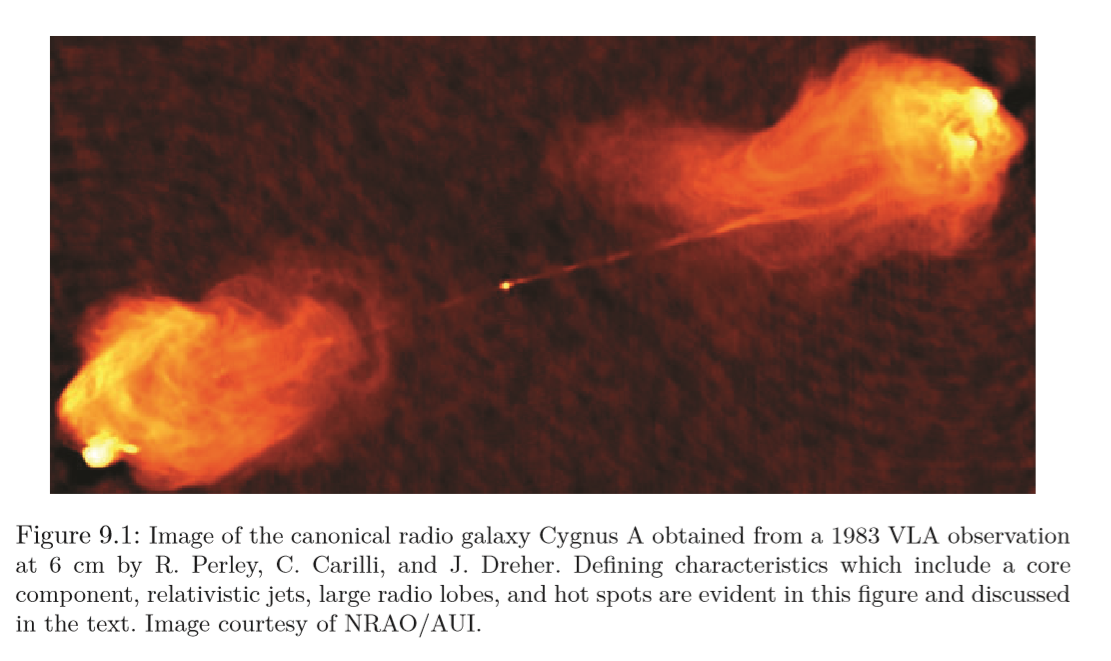
\includegraphics[scale=1]{cygnus.png}
 \end{figure}
 Higher resolution and more sensitive radio observations in the 1970s revealed compact sources of radio emission in the cores of many of these galaxies and that the lobes are connected to the core of the host galaxy by long thin lines of faint radiation; these features are also apparent in Figure \ref{cygnus}. These lines, now referred to as jets, are streams of particles ejected from the nuclei of these galaxies at relativistic speeds. Also apparent in Figure \ref{cygnus} in the lobes, are bright spots of emission; these hot spots are believed to be collision sites between the jet particles and the extragalactic medium. \\

\tbf{Q. Features of radio galaxies through observation and what we can infer from spectral emission observation}\\

The huge intensities of the radio emission from radio galaxies lead to absurdly large brightness temperatures,implying that this radiation is produced by non-thermal processes. Additionally, the radio spectra of these galaxies are found to follow decreasing power laws (see Figure \ref{radiosyn}) and so they are inferred to be synchrotron radiation sources \\ 
\begin{figure}[h!]\label{radiosyn}
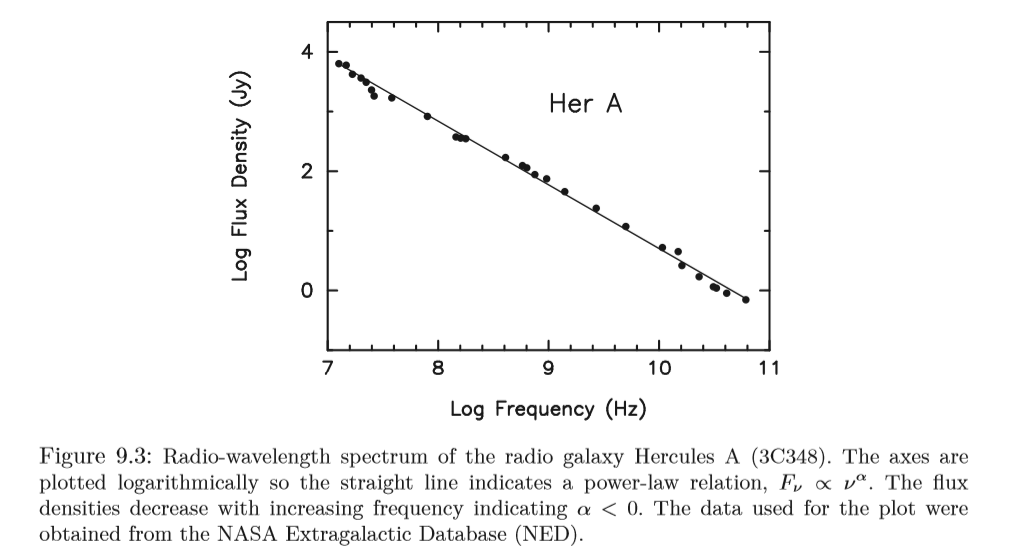
\includegraphics[scale=1]{radiosyn.png}
\end{figure}
The synchrotron emission will be dominated by the lowest-mass charged particles, which at least include electrons. The jets may also include positrons, but since the emission from positrons would be identical to that from electrons, we can model the observed radiation considering only electrons. Since these objects must be electrically neutral, we know that positive charges, be they protons or positrons, must be contained in the same volume. \\

\tbf{Q.  emission of radio galaxies .}\\

The decreasing power-law spectra can be represented mathematically by
\begin{equation}
F_\nu \propto \nu_\alpha
\end{equation}
where $\alpha$ is the spectral index.  For decreasing flux density with increasing frequency $\alpha$ is negative.\\

\tbf{Q.  QSO's as primordial Radio galaxies }\\

Today we know them as quasars, these super bright galaxies. When they were first discovered  These objects were, therefore, the most distant objects known at that time. They were so far away that not only would ordinary stars be impossible to detect but even whole galaxies would appear quite faint. Therefore, these quasi-stellar objects were inferred to be very luminous active nuclei of distant galaxies,whose stellar component was not detected in the glare of the bright core. Although they appear as faint as ordinary stars, taking into account their distances, the luminosities of these AGN can be as large as hundreds of times that of the entire Milky Way galaxy.  Repeated imaging of quasars with extremely high resolution radio observations using very long baseline interferometry techniques revealed significant outward motions (see discussion in Section 9.4.2), confirming that these objects contain radio jets.



\tbf{Q. Do you find QSO's everywhere?}

Quasars,as a rule,are found at large redshifts.\\

The number density of quasars per unit volume is found to increase toward higher redshifts, peaking between redshifts of 1 and 2. Active galactic nuclei, in general, are more common at higher redshifts, typically with higher luminosities at higher redshifts. The redshift distribution depends on the particular defining AGN parameters and on the limitations of the survey, but the tendency for AGN to be more common in the past is definite in all studies. 

\tbf{Let us determine some parameters relating to the radio quasar.}\\
\tbf{Sample problem: The quasar 3C273 has a redshift z=0.158. What is the look-back time for observations of this object?Assume $H_0 =2.27\times 10^{-18} s^{-1}, \Omega_M =0.3 \text{ and } \Omega_\Lambda =0.7$. What is the proper distance to 3C273? }\\

Answer.  We first need the age of the Universe when light with redshift z was emitted, which is given by Equation
\begin{equation}
t_e=11.1 \sinh^{-1}\rr{\frac{1.53}{\cc{1+0.159}^{3/2}}}Gyr=11.5Gyr
\end{equation}
Since the current age of the Universe assuming these cosmological parameter values is about 13.5 Gyr, the look-back time for this object is 2 billion years. \\

Calculating cosmological distances can be cumbersome because it requires a numerical integration, and a common temptation is to use the Hubble-Lemaıtre law (which works for low redshifts) approximation to roughly estimate the distance. If we do that with 3C273 we get 
\begin{equation}
d=\frac{cz}{H_0}=\frac{0.158 \times 3 \times 10^5 Km s^{-1}}{70 km s^{-1} Mpc^{-1}}=677Mpc
\end{equation}
\tbf{Note: The error in estimate based on the Hubble-Lemaıtre law approximation increases with increasing redshift}\\

\tbf{Q. Sample Problem: The flux we detect from 3C273 in just the visible window is approximately $2.1\times 10{-10} erg s^{-1} cm{-2}$. Calculate the luminosity of the radiation we detect in the visible from 3C273. (Note, because of its redshift, some of the radiation we detect in the visible is emitted in the ultraviolet. This question asks us to focus only the radiation we detect in the visible.) Convert the answer to solar luminosities. }\\

The luminosity relates to detected flux by
\begin{equation}
L^{V}=F^{V}\times 4 \pi d_L^2=\cc{2.1 \times 10^{-10}erg \;\; s^{-1}cm^{-2}}\times\cc{4 \pi D_L^2}
\end{equation}
where the superscript V indicates flux and luminosity only in the visible window, and $d_L$,3C273 is the luminosity distance of 3C273.\\

 We use the luminosity distance because we are converting flux to luminosity. The luminosity distance is related to the proper distance. The luminosity distance, then, is 
 \begin{equation}
 d_L=6.52 \times 10^8 pc\cc{1+0.158}=7.55 \times10^8pc=2.33 \times 10^{27} cm
 \end{equation}
Putting this value for $d_L$,3C273 into the equation we get 
 \begin{equation}
 L^V=\cc{2.1 \times 10^{-10}erg \;\; s^{-1}cm^{-2}}4 \pi \cc{2.33 \times 10^{27cm}}^2\\
 =1.43\times10^{46}erg\;s^{-1} 
 \end{equation}
 the radiation output of 3C273 at visible wavelengths is on the order of that emitted by about a hundred Milky Way galaxies!\\
 
 \section{The AGN model}
 \tbf{Q. What is structure of  AGN as we know through observations?}\\
 The model of an active galactic nucleus involves the infall of gas towards a supermassive black hole, generally with $M \sim10^6\text{ to }10^9 M_\odot$. The heating of gas as it spirals in toward a black hole is an efficient mechanism for converting gravitational potential energy into radiation. Numerous studies of the kinematics of the central regions of galaxies provide strong evidence that supermassive black holes commonly exist in galactic centers. As the interstellar gas falls inward, its angular momentum causes it to form a rotating disk of gas around the blackhole;this is termed an accretion disk.Because of conservation of energy,as the gas falls inward its gravitational potential energy is converted to kinetic energy which is converted by collisions of the gas in the disk to thermal energy.The accretion disk,therefore, is heated to high temperatures with higher temperatures at smaller radii,closer to the black hole. By the time the gas gets close to the black hole it is sufficiently hot to emit X-rays. \\
 
 But this was about the core,\\
 In addition to the small size of the central engine, AGN models must also explain the jets of particles streaming away from the black hole at relativistic speeds. Currently no model for the formation of jets has successfully explained all the details,but the mechanism necessarily involves a combination of magneto-hydrodynamics and general relativity.\\
 
 \tbf{Q. How would we explain the jets}\\ 
   One of the more successful models was developed by Roger Blandford and Roman Znajek, in which rotational energy of the black hole is tapped to power the jets. The material that falls into the black hole carries large amounts of angular momentum with it, so that over millions of years the black hole obtains a large rotation rate.The in falling matter also carries along a magnetic field that intensifies as the gas collapses to smaller volumes. Recall that the intense synchrotron radiation we detect from these sources requires that they contain strong magnetic fields. A rotating supermassive black hole in a magnetic field produces an interesting effect related to formation of the radio jets.\\
    \tbf{ By the Blandford-Znajek effect, just outside the black hole an electric field is induced, which accelerates charges away from the black hole. These charges get attached to open magnetic field lines, which will be twisted into helical shapes. The points where the magnetic field lines are anchored to the rotating matter are dragged along in the rotation, but because of the finite speed of transfer of information about the rotation, the field lines further out are delayed in their rotation. The bases of the field lines, then, twist ahead of the lines further out and so the open magnetic field lines at the poles end up as helices, as shown in Figure \ref{bzeffect} We can think of a charged particle following a magnetic field line similar in behavior to a bead on a wire}.\\
    
     Imagine a wire bent into a helical shape increasing in diameter with distance from its base, oriented vertically with the small end at the floor, and rotating at high speeds about its axis. The bead will be swung outward and upward. A charged particle attached to an open, helical magnetic field line of a rotating system, similarly, will be pushed outward and accelerated away from the black hole.An aspect of the jets that is more difficult to explain theoretically is how the magnetic field lines and path of ejected particles are focused into and remain in finely-collimated beams. 
   \begin{figure}\label{bzeffect}
   \includegraphics[scale=1]{thebzeffect.png}
   \end{figure}
\end{document}